%&preformat-disser
\RequirePackage[l2tabu,orthodox]{nag} % Раскомментировав, можно в логе получать рекомендации относительно правильного использования пакетов и предупреждения об устаревших и нерекомендуемых пакетах
% Формат А4, 14pt (ГОСТ Р 7.0.11-2011, 5.3.6)
\documentclass[a4paper,14pt,oneside,openany]{memoir}

%%%%%%%%%%%%%%%%%%%%%%%%%%%%%%%%%%%%%%%%%%%%%%%%%%%%%%
%%%% Файл упрощённых настроек шаблона диссертации %%%%
%%%%%%%%%%%%%%%%%%%%%%%%%%%%%%%%%%%%%%%%%%%%%%%%%%%%%%

%%% Инициализирование переменных, не трогать!  %%%
\newcounter{tabcap}
\newcounter{tablaba}
\newcounter{tabtita}
\newcounter{showperssign}
\newcounter{showsecrsign}
\newcounter{showopplead}
\newcounter{usefootcite}
%%%%%%%%%%%%%%%%%%%%%%%%%%%%%%%%%%%%%%%%%%%%%%%%%%

%%% Область упрощённого управления оформлением %%%

%% Управление зазором между подрисуночной подписью и основным текстом
\setlength{\belowcaptionskip}{10pt plus 20pt minus 2pt}


%% Подпись таблиц
\setcounter{tabcap}{0}              % 0 --- по ГОСТ, номер таблицы и название разделены тире, выровнены по левому краю, при необходимости на нескольких строках; 1 --- подпись таблицы не по ГОСТ, на двух и более строках, дальнейшие настройки: 
%Выравнивание первой строки, с подписью и номером
\setcounter{tablaba}{2}             % 0 --- по левому краю; 1 --- по центру; 2 --- по правому краю
%Выравнивание строк с самим названием таблицы
\setcounter{tabtita}{1}             % 0 --- по левому краю; 1 --- по центру; 2 --- по правому краю
%Разделитель записи «Таблица #» и названия таблицы
\newcommand{\tablabelsep}{ }

%% Подпись рисунков
%Разделитель записи «Рисунок #» и названия рисунка
\newcommand{\figlabelsep}{~\cyrdash\ } % (ГОСТ 2.105, 4.3.1) % "--- здесь не работает

%Демонстрация подписи диссертанта на автореферате
\setcounter{showperssign}{1}        % 0 --- не показывать; 1 --- показывать
%Демонстрация подписи учёного секретаря на автореферате
\setcounter{showsecrsign}{1}        % 0 --- не показывать; 1 --- показывать
%Демонстрация информации об оппонентах и ведущей организации на автореферате
\setcounter{showopplead}{1}         % 0 --- не показывать; 1 --- показывать

%%% Цвета гиперссылок %%%
% Latex color definitions: http://latexcolor.com/
%\definecolor{linkcolor}{rgb}{0.9,0,0}
%\definecolor{citecolor}{rgb}{0,0.6,0}
%\definecolor{urlcolor}{rgb}{0,0,1}
\definecolor{linkcolor}{rgb}{0,0,0} %black
\definecolor{citecolor}{rgb}{0,0,0} %black
\definecolor{urlcolor}{rgb}{0,0,0} %black

%%% Библиография
\setcounter{usefootcite}{0}         % 0 --- два списка литературы, 1 --- список публикаций автора + цитирование других работ в сносках
            % общие настройки шаблона
\input{common/packages}         % Пакеты общие для диссертации и автореферата
\synopsisfalse                      % Этот документ --- не автореферат
\input{Dissertation/dispackages}    % Пакеты для диссертации
\input{Dissertation/userpackages}   % Пакеты для специфических пользовательских задач

%%%%%%%%%%%%%%%%%%%%%%%%%%%%%%%%%%%%%%%%%%%%%%%%%%%%%%
%%%% Файл упрощённых настроек шаблона диссертации %%%%
%%%%%%%%%%%%%%%%%%%%%%%%%%%%%%%%%%%%%%%%%%%%%%%%%%%%%%

%%% Инициализирование переменных, не трогать!  %%%
\newcounter{intvl}
\newcounter{otstup}
\newcounter{contnumeq}
\newcounter{contnumfig}
\newcounter{contnumtab}
\newcounter{pgnum}
\newcounter{chapstyle}
\newcounter{headingdelim}
\newcounter{headingalign}
\newcounter{headingsize}
\newcounter{tabcap}
\newcounter{tablaba}
\newcounter{tabtita}
\newcounter{usefootcite}
%%%%%%%%%%%%%%%%%%%%%%%%%%%%%%%%%%%%%%%%%%%%%%%%%%

%%% Область упрощённого управления оформлением %%%

%% Интервал между заголовками и между заголовком и текстом
% Заголовки отделяют от текста сверху и снизу тремя интервалами (ГОСТ Р 7.0.11-2011, 5.3.5)
\setcounter{intvl}{3}               % Коэффициент кратности к размеру шрифта

%% Отступы у заголовков в тексте
\setcounter{otstup}{0}              % 0 --- без отступа; 1 --- абзацный отступ

%% Нумерация формул, таблиц и рисунков
\setcounter{contnumeq}{0}           % Нумерация формул: 0 --- пораздельно (во введении подряд, без номера раздела); 1 --- сквозная нумерация по всей диссертации
\setcounter{contnumfig}{0}          % Нумерация рисунков: 0 --- пораздельно (во введении подряд, без номера раздела); 1 --- сквозная нумерация по всей диссертации
\setcounter{contnumtab}{1}          % Нумерация таблиц: 0 --- пораздельно (во введении подряд, без номера раздела); 1 --- сквозная нумерация по всей диссертации

%% Оглавление
\setcounter{pgnum}{1}               % 0 --- номера страниц никак не обозначены; 1 --- Стр. над номерами страниц (дважды компилировать после изменения)
\settocdepth{subsection}            % до какого уровня подразделов выносить в оглавление
\setsecnumdepth{subsection}         % до какого уровня нумеровать подразделы


%% Текст и форматирование заголовков
\setcounter{chapstyle}{1}           % 0 --- разделы только под номером; 1 --- разделы с названием "Глава" перед номером
\setcounter{headingdelim}{1}        % 0 --- номер отделен пропуском в 1em или \quad; 1 --- номера разделов и приложений отделены точкой с пробелом, подразделы пропуском без точки; 2 --- номера разделов, подразделов и приложений отделены точкой с пробелом.

%% Выравнивание заголовков в тексте
\setcounter{headingalign}{0}        % 0 --- по центру; 1 --- по левому краю

%% Размеры заголовков в тексте
\setcounter{headingsize}{0}         % 0 --- по ГОСТ, все всегда 14 пт; 1 --- пропорционально изменяющийся размер в зависимости от базового шрифта

%% Подпись таблиц
\setcounter{tabcap}{0}              % 0 --- по ГОСТ, номер таблицы и название разделены тире, выровнены по левому краю, при необходимости на нескольких строках; 1 --- подпись таблицы не по ГОСТ, на двух и более строках, дальнейшие настройки: 
%Выравнивание первой строки, с подписью и номером
\setcounter{tablaba}{2}             % 0 --- по левому краю; 1 --- по центру; 2 --- по правому краю
%Выравнивание строк с самим названием таблицы
\setcounter{tabtita}{1}             % 0 --- по левому краю; 1 --- по центру; 2 --- по правому краю
%Разделитель записи «Таблица #» и названия таблицы
\newcommand{\tablabelsep}{ }

%% Подпись рисунков
%Разделитель записи «Рисунок #» и названия рисунка
\newcommand{\figlabelsep}{~\cyrdash\ } % (ГОСТ 2.105, 4.3.1) % "--- здесь не работает

%%% Цвета гиперссылок %%%
% Latex color definitions: http://latexcolor.com/
%\definecolor{linkcolor}{rgb}{0.9,0,0}
%\definecolor{citecolor}{rgb}{0,0.6,0}
%\definecolor{urlcolor}{rgb}{0,0,1}
\definecolor{linkcolor}{rgb}{0,0,0} %black
\definecolor{citecolor}{rgb}{0,0,0} %black
\definecolor{urlcolor}{rgb}{0,0,0} %black
      % Упрощённые настройки шаблона

\input{common/newnames}         % Новые переменные, для всего проекта

%%% Основные сведения %%%
\newcommand{\thesisAuthorLastName}{Куликова}%\todo{Куликова}}
\newcommand{\thesisAuthorOtherNames}{Агриппина Михайловна}
\newcommand{\thesisAuthorInitials}{А.\,М.}
\newcommand{\thesisAuthor}             % Диссертация, ФИО автора
{%
    \texorpdfstring{% \texorpdfstring takes two arguments and uses the first for (La)TeX and the second for pdf
        \thesisAuthorLastName~\thesisAuthorOtherNames% так будет отображаться на титульном листе или в тексте, где будет использоваться переменная
    }{%
        \thesisAuthorLastName, \thesisAuthorOtherNames% эта запись для свойств pdf-файла. В таком виде, если pdf будет обработан программами для сбора библиографических сведений, будет правильно представлена фамилия.
    }
}
\newcommand{\thesisAuthorShort}        % Диссертация, ФИО автора инициалами
{\thesisAuthorInitials~\thesisAuthorLastName}
%\newcommand{\thesisUdk}                % Диссертация, УДК
%{\todo{xxx.xxx}}
\newcommand{\thesisTitle}              % Диссертация, название
%{АСТРОМЕТРИЧЕСКИЕ ДВОЙНЫЕ СРЕДИ ЗВЕЗД НИЗКОЙ СВЕТИМОСТИ}
{Астрометрические двойные \\среди звезд низкой светимости}
\newcommand{\thesisSpecialtyNumber}    % Диссертация, специальность, номер
{01.03.01}
\newcommand{\thesisSpecialtyTitle}     % Диссертация, специальность, название (название взято с сайта ВАК для примера)
{Астрометрия и Небесная механика}
%% \newcommand{\thesisSpecialtyTwoNumber} % Диссертация, вторая специальность, номер
%% {\todo{XX.XX.XX}}
%% \newcommand{\thesisSpecialtyTwoTitle}  % Диссертация, вторая специальность, название
%% {\todo{Теория и~методика физического воспитания, спортивной тренировки,
%% оздоровительной и~адаптивной физической культуры}}
\newcommand{\thesisDegree}             % Диссертация, ученая степень
{кандидата физико-математических наук}
\newcommand{\thesisDegreeShort}        % Диссертация, ученая степень, краткая запись
{канд. физ.-мат. наук}
\newcommand{\thesisCity}               % Диссертация, город написания диссертации
{Санкт-Петербург}
\newcommand{\thesisYear}               % Диссертация, год написания диссертации
{2019}
\newcommand{\thesisOrganization}       % Диссертация, организация
{Федеральное государственное бюджетное учреждение науки \\*
 <<Главная (Пулковская) астрономическая обсерватория \\*Российской академии наук}% \\* <<ГАО РАН>>}
\newcommand{\thesisOrganizationShort}  % Диссертация, краткое название организации для доклада
{ГАО РАН}

\newcommand{\thesisInOrganization}     % Диссертация, организация в предложном падеже: Работа выполнена в ...
{Федеральном государственном бюджетном учреждении науки
 <<Главной (Пулковской) астрономической обсерватории Российской академии наук}

%% \newcommand{\supervisorDead}{}           % Рисовать рамку вокруг фамилии
\newcommand{\supervisorFio}              % Научный руководитель, ФИО
{Ховричев Максим Юрьевич}
\newcommand{\supervisorRegalia}          % Научный руководитель, регалии
{к.ф.-м.н., снс, ИО зав. ЛАЗА ГАО РАН}
\newcommand{\supervisorFioShort}         % Научный руководитель, ФИО
{М.\,Ю.~Ховричев}
\newcommand{\supervisorRegaliaShort}     % Научный руководитель, регалии
{к.ф.-м.н.}
%% \newcommand{\supervisorTwoDead}{}        % Рисовать рамку вокруг фамилии
%% \newcommand{\supervisorTwoFio}           % Второй научный руководитель, ФИО
%% {\todo{Фамилия Имя Отчество}}
%% \newcommand{\supervisorTwoRegalia}       % Второй научный руководитель, регалии
%% {\todo{уч. степень, уч. звание}}
%% \newcommand{\supervisorTwoFioShort}      % Второй научный руководитель, ФИО
%% {\todo{И.\,О.~Фамилия}}
%% \newcommand{\supervisorTwoRegaliaShort}  % Второй научный руководитель, регалии
%% {\todo{уч.~ст.,~уч.~зв.}}

\newcommand{\opponentOneFio}           % Оппонент 1, ФИО
{\todo{Фамилия Имя Отчество}}
\newcommand{\opponentOneRegalia}       % Оппонент 1, регалии
{\todo{доктор физико-математических наук, профессор}}
\newcommand{\opponentOneJobPlace}      % Оппонент 1, место работы
{\todo{Не очень длинное название для места работы}}
\newcommand{\opponentOneJobPost}       % Оппонент 1, должность
{\todo{старший научный сотрудник}}

\newcommand{\opponentTwoFio}           % Оппонент 2, ФИО
{\todo{Фамилия Имя Отчество}}
\newcommand{\opponentTwoRegalia}       % Оппонент 2, регалии
{\todo{кандидат физико-математических наук}}
\newcommand{\opponentTwoJobPlace}      % Оппонент 2, место работы
{\todo{Основное место работы c длинным длинным длинным длинным названием}}
\newcommand{\opponentTwoJobPost}       % Оппонент 2, должность
{\todo{старший научный сотрудник}}

%% \newcommand{\opponentThreeFio}         % Оппонент 3, ФИО
%% {\todo{Фамилия Имя Отчество}}
%% \newcommand{\opponentThreeRegalia}     % Оппонент 3, регалии
%% {\todo{кандидат физико-математических наук}}
%% \newcommand{\opponentThreeJobPlace}    % Оппонент 3, место работы
%% {\todo{Основное место работы c длинным длинным длинным длинным названием}}
%% \newcommand{\opponentThreeJobPost}     % Оппонент 3, должность
%% {\todo{старший научный сотрудник}}

\newcommand{\leadingOrganizationTitle} % Ведущая организация, дополнительные строки. Удалить, чтобы не отображать в автореферате
{\todo{Федеральное государственное бюджетное образовательное учреждение высшего
профессионального образования с~длинным длинным длинным длинным названием}}

\newcommand{\defenseDate}              % Защита, дата
{\todo{DD mmmmmmmm YYYY~г.~в~XX часов}}
\newcommand{\defenseCouncilNumber}     % Защита, номер диссертационного совета
{\todo{Д\,123.456.78}}
\newcommand{\defenseCouncilTitle}      % Защита, учреждение диссертационного совета
{\todo{Название учреждения}}
\newcommand{\defenseCouncilAddress}    % Защита, адрес учреждение диссертационного совета
{\todo{Адрес}}
\newcommand{\defenseCouncilPhone}      % Телефон для справок
{\todo{+7~(0000)~00-00-00}}

\newcommand{\defenseSecretaryFio}      % Секретарь диссертационного совета, ФИО
{\todo{Фамилия Имя Отчество}}
\newcommand{\defenseSecretaryRegalia}  % Секретарь диссертационного совета, регалии
{\todo{д-р~физ.-мат. наук}}            % Для сокращений есть ГОСТы, например: ГОСТ Р 7.0.12-2011 + http://base.garant.ru/179724/#block_30000

\newcommand{\synopsisLibrary}          % Автореферат, название библиотеки
{\todo{Название библиотеки}}
\newcommand{\synopsisDate}             % Автореферат, дата рассылки
{\todo{DD mmmmmmmm YYYY года}}

% To avoid conflict with beamer class use \providecommand
\providecommand{\keywords}%            % Ключевые слова для метаданных PDF диссертации и автореферата
{}
             % Основные сведения
\input{common/fonts}            % Определение шрифтов (частичное)
\input{common/styles}           % Стили общие для диссертации и автореферата
\input{Dissertation/disstyles}  % Стили для диссертации
\input{Dissertation/userstyles} % Стили для специфических пользовательских задач

%%% Библиография. Выбор движка для реализации %%%
\ifnumequal{\value{bibliosel}}{0}{%
    %%% Реализация библиографии встроенными средствами посредством движка bibtex8 %%%

%%% Пакеты %%%
\usepackage{cite}                                   % Красивые ссылки на литературу


%%% Стили %%%
\bibliographystyle{BibTeX-Styles/utf8gost71u}    % Оформляем библиографию по ГОСТ 7.1 (ГОСТ Р 7.0.11-2011, 5.6.7)

\makeatletter
\renewcommand{\@biblabel}[1]{#1.}   % Заменяем библиографию с квадратных скобок на точку
\makeatother
%% Управление отступами между записями
%% требует etoolbox
%% http://tex.stackexchange.com/a/105642
%\patchcmd\thebibliography
% {\labelsep}
% {\labelsep\itemsep=5pt\parsep=0pt\relax}
% {}
% {\typeout{Couldn't patch the command}}

%%% Список литературы с красной строки (без висячего отступа) %%%
%\patchcmd{\thebibliography} %может потребовать включения пакета etoolbox
%  {\advance\leftmargin\labelsep}
%  {\leftmargin=0pt%
%   \setlength{\labelsep}{\widthof{\ }}% Управляет длиной отступа после точки
%   \itemindent=\parindent%
%   \addtolength{\itemindent}{\labelwidth}% Сдвигаем правее на величину номера с точкой
%   \advance\itemindent\labelsep%
%  }
%  {}{}

%%% Цитирование %%%
\renewcommand\citepunct{;\penalty\citepunctpenalty%
    \hskip.13emplus.1emminus.1em\relax}                % Разделение ; при перечислении ссылок (ГОСТ Р 7.0.5-2008)

\newcommand*{\autocite}{\cite}  % Чтобы примеры цитирования, рассчитанные на biblatex, не вызывали ошибок при компиляции в bibtex

%%% Создание команд для вывода списка литературы %%%
\newcommand*{\insertbibliofull}{
\bibliography{biblio/external,biblio/authorvak,biblio/authorscopus,biblio/authorwos,biblio/authorother,biblio/authorconf}         % Подключаем BibTeX-базы % После запятых не должно быть лишних пробелов — он "думает", что это тоже имя пути
}

\newcommand*{\insertbiblioauthor}{
\bibliography{biblio/authorvak,biblio/authorscopus,biblio/authorwos,biblio/authorother,biblio/authorconf}         % Подключаем BibTeX-базы % После запятых не должно быть лишних пробелов — он "думает", что это тоже имя пути
}

\newcommand*{\insertbiblioexternal}{
\bibliography{biblio/external}         % Подключаем BibTeX-базы
}


%% Счётчик использованных ссылок на литературу, обрабатывающий с учётом неоднократных ссылок
%% Требуется дважды компилировать, поскольку ему нужно считать актуальный внешний файл со списком литературы
\newtotcounter{citenum}
\def\oldcite{}
\let\oldcite=\bibcite
\def\bibcite{\stepcounter{citenum}\oldcite}
   % Встроенная реализация с загрузкой файла через движок bibtex8
}{
    %%% Реализация библиографии пакетами biblatex и biblatex-gost с использованием движка biber %%%

\usepackage{csquotes} % biblatex рекомендует его подключать. Пакет для оформления сложных блоков цитирования.
%%% Загрузка пакета с основными настройками %%%
\makeatletter
\ifnumequal{\value{draft}}{0}{% Чистовик
\usepackage[%
backend=biber,% движок
bibencoding=utf8,% кодировка bib файла
sorting=none,% настройка сортировки списка литературы
style=gost-numeric,% стиль цитирования и библиографии (по ГОСТ)
language=autobib,% получение языка из babel/polyglossia, default: autobib % если ставить autocite или auto, то цитаты в тексте с указанием страницы, получат указание страницы на языке оригинала
autolang=other,% многоязычная библиография
clearlang=true,% внутренний сброс поля language, если он совпадает с языком из babel/polyglossia
defernumbers=true,% нумерация проставляется после двух компиляций, зато позволяет выцеплять библиографию по ключевым словам и нумеровать не из большего списка
sortcites=true,% сортировать номера затекстовых ссылок при цитировании (если в квадратных скобках несколько ссылок, то отображаться будут отсортированно, а не абы как)
doi=false,% Показывать или нет ссылки на DOI
isbn=false,% Показывать или нет ISBN, ISSN, ISRN
]{biblatex}[2016/09/17]
\ltx@iffilelater{biblatex-gost.def}{2017/05/03}%
{%\toggletrue{bbx:gostbibliography}%
\renewcommand*{\revsdnamepunct}{\addcomma}}{}
}{%Черновик
\usepackage[%
backend=biber,% движок
bibencoding=utf8,% кодировка bib файла
sorting=none,% настройка сортировки списка литературы
]{biblatex}[2016/09/17]%
}
\makeatother

\ifnumgreater{\value{usefootcite}}{0}{
    \ExecuteBibliographyOptions{autocite=footnote}
    \newbibmacro*{cite:full}{%
        \printtext[bibhypertarget]{%
            \usedriver{%
                \DeclareNameAlias{sortname}{default}%
            }{%
                \thefield{entrytype}%
            }%
        }%
        \usebibmacro{shorthandintro}%
    }
    \DeclareCiteCommand{\smartcite}[\mkbibfootnote]{%
        \usebibmacro{prenote}%
    }{%
        \usebibmacro{citeindex}%
        \usebibmacro{cite:full}%
    }{%
        \multicitedelim%
    }{%
        \usebibmacro{postnote}%
    }
}{}

%%% Подключение файлов bib %%%
\addbibresource[label=bl-external]{biblio/external.bib}
\addbibresource[label=bl-authorvak]{biblio/authorvak.bib}
\addbibresource[label=bl-authorscopus]{biblio/authorscopus.bib}
\addbibresource[label=bl-authorwos]{biblio/authorwos.bib}
\addbibresource[label=bl-authorother]{biblio/authorother.bib}
\addbibresource[label=bl-authorconf]{biblio/authorconf.bib}


%http://tex.stackexchange.com/a/141831/79756
%There is a way to automatically map the language field to the langid field. The following lines in the preamble should be enough to do that.
%This command will copy the language field into the langid field and will then delete the contents of the language field. The language field will only be deleted if it was successfully copied into the langid field.
\DeclareSourcemap{ %модификация bib файла перед тем, как им займётся biblatex
    \maps{
        \map{% перекидываем значения полей language в поля langid, которыми пользуется biblatex
            \step[fieldsource=language, fieldset=langid, origfieldval, final]
            \step[fieldset=language, null]
        }
        \map[overwrite]{% перекидываем значения полей shortjournal, если они есть, в поля journal, которыми пользуется biblatex
            \step[fieldsource=shortjournal, final]
            \step[fieldset=journal, origfieldval]
        }
        \map[overwrite]{% перекидываем значения полей shortbooktitle, если они есть, в поля booktitle, которыми пользуется biblatex
            \step[fieldsource=shortbooktitle, final]
            \step[fieldset=booktitle, origfieldval]
        }
        \map[overwrite, refsection=0]{% стираем значения всех полей addendum
            \perdatasource{biblio/authorvak.bib}
            \perdatasource{biblio/authorscopus.bib}
            \perdatasource{biblio/authorwos.bib}
            \perdatasource{biblio/authorother.bib}
            \perdatasource{biblio/authorconf.bib}
            \step[fieldsource=addendum, final]
            \step[fieldset=addendum, null] %чтобы избавиться от информации об объёме авторских статей, в отличие от автореферата
        }
        \map[overwrite]{% перекидываем refbase в addendum, чтобы указать тип публикации (ВАК, Scopus, WoS) в конце ссылки
            \perdatasource{biblio/authorvak.bib}
            \perdatasource{biblio/authorscopus.bib}
            \perdatasource{biblio/authorwos.bib}
            \step[fieldsource=refbase, final]
            \step[fieldset=addendum, origfieldval]
        }
        \map{% перекидываем значения полей numpages в поля pagetotal, которыми пользуется biblatex
            \step[fieldsource=numpages, fieldset=pagetotal, origfieldval, final]
            \step[fieldset=pagestotal, null]
        }
        \map{% если в поле medium написано "Электронный ресурс", то устанавливаем поле media, которым пользуется biblatex, в значение eresource.
            \step[fieldsource=medium,
            match=\regexp{Электронный\s+ресурс},
            final]
            \step[fieldset=media, fieldvalue=eresource]
        }
        \map[overwrite]{% стираем значения всех полей issn
            \step[fieldset=issn, null]
        }
        \map[overwrite]{% стираем значения всех полей abstract, поскольку ими не пользуемся, а там бывают "неприятные" латеху символы
            \step[fieldsource=abstract]
            \step[fieldset=abstract,null]
        }
        \map[overwrite]{ % переделка формата записи даты
            \step[fieldsource=urldate,
            match=\regexp{([0-9]{2})\.([0-9]{2})\.([0-9]{4})},
            replace={$3-$2-$1$4}, % $4 вставлен исключительно ради нормальной работы программ подсветки синтаксиса, которые некорректно обрабатывают $ в таких конструкциях
            final]
        }
        \map[overwrite]{ % добавляем ключевые слова, чтобы различать источники
            \perdatasource{biblio/external.bib}
            \step[fieldset=keywords, fieldvalue={biblioexternal,bibliofull}]
        }
        \map[overwrite]{ % добавляем ключевые слова, чтобы различать источники
            \perdatasource{biblio/authorvak.bib}
            \step[fieldset=keywords, fieldvalue={biblioauthorvak,biblioauthor,bibliofull}]
        }
        \map[overwrite]{ % добавляем ключевые слова, чтобы различать источники
            \perdatasource{biblio/authorscopus.bib}
            \step[fieldset=keywords, fieldvalue={biblioauthorscopus,biblioauthor,bibliofull}]
        }
        \map[overwrite]{ % добавляем ключевые слова, чтобы различать источники
            \perdatasource{biblio/authorwos.bib}
            \step[fieldset=keywords, fieldvalue={biblioauthorwos,biblioauthor,bibliofull}]
        }
        \map[overwrite]{ % добавляем ключевые слова, чтобы различать источники
            \perdatasource{biblio/authorother.bib}
            \step[fieldset=keywords, fieldvalue={biblioauthorother,biblioauthor,bibliofull}]
        }
        \map[overwrite]{ % добавляем ключевые слова, чтобы различать источники
            \perdatasource{biblio/authorconf.bib}
            \step[fieldset=keywords, fieldvalue={biblioauthorconf,biblioauthor,bibliofull}]
        }
%        \map[overwrite]{% стираем значения всех полей series
%            \step[fieldset=series, null]
%        }
        \map[overwrite]{% перекидываем значения полей howpublished в поля organization для типа online
            \step[typesource=online, typetarget=online, final]
            \step[fieldsource=howpublished, fieldset=organization, origfieldval]
            \step[fieldset=howpublished, null]
        }
        % Так отключаем [Электронный ресурс]
%        \map[overwrite]{% стираем значения всех полей media=eresource
%            \step[fieldsource=media,
%            match={eresource},
%            final]
%            \step[fieldset=media, null]
%        }
    }
}

%%% Убираем неразрывные пробелы перед двоеточием и точкой с запятой %%%
%\makeatletter
%\ifnumequal{\value{draft}}{0}{% Чистовик
%    \renewcommand*{\addcolondelim}{%
%      \begingroup%
%      \def\abx@colon{%
%        \ifdim\lastkern>\z@\unkern\fi%
%        \abx@puncthook{:}\space}%
%      \addcolon%
%      \endgroup}
%
%    \renewcommand*{\addsemicolondelim}{%
%      \begingroup%
%      \def\abx@semicolon{%
%        \ifdim\lastkern>\z@\unkern\fi%
%        \abx@puncthook{;}\space}%
%      \addsemicolon%
%      \endgroup}
%}{}
%\makeatother

%%% Правка записей типа thesis, чтобы дважды не писался автор
%\ifnumequal{\value{draft}}{0}{% Чистовик
%\DeclareBibliographyDriver{thesis}{%
%  \usebibmacro{bibindex}%
%  \usebibmacro{begentry}%
%  \usebibmacro{heading}%
%  \newunit
%  \usebibmacro{author}%
%  \setunit*{\labelnamepunct}%
%  \usebibmacro{thesistitle}%
%  \setunit{\respdelim}%
%  %\printnames[last-first:full]{author}%Вот эту строчку нужно убрать, чтобы автор диссертации не дублировался
%  \newunit\newblock
%  \printlist[semicolondelim]{specdata}%
%  \newunit
%  \usebibmacro{institution+location+date}%
%  \newunit\newblock
%  \usebibmacro{chapter+pages}%
%  \newunit
%  \printfield{pagetotal}%
%  \newunit\newblock
%  \usebibmacro{doi+eprint+url+note}%
%  \newunit\newblock
%  \usebibmacro{addendum+pubstate}%
%  \setunit{\bibpagerefpunct}\newblock
%  \usebibmacro{pageref}%
%  \newunit\newblock
%  \usebibmacro{related:init}%
%  \usebibmacro{related}%
%  \usebibmacro{finentry}}
%}{}

%\newbibmacro{string+doi}[1]{% новая макрокоманда на простановку ссылки на doi
%    \iffieldundef{doi}{#1}{\href{http://dx.doi.org/\thefield{doi}}{#1}}}

%\ifnumequal{\value{draft}}{0}{% Чистовик
%\renewcommand*{\mkgostheading}[1]{\usebibmacro{string+doi}{#1}} % ссылка на doi с авторов. стоящих впереди записи
%\renewcommand*{\mkgostheading}[1]{#1} % только лишь убираем курсив с авторов
%}{}
%\DeclareFieldFormat{title}{\usebibmacro{string+doi}{#1}} % ссылка на doi с названия работы
%\DeclareFieldFormat{journaltitle}{\usebibmacro{string+doi}{#1}} % ссылка на doi с названия журнала
%%% Тире как разделитель в библиографии традиционной руской длины:
\renewcommand*{\newblockpunct}{\addperiod\addnbspace\cyrdash\space\bibsentence}
%%% Убрать тире из разделителей элементов в библиографии:
%\renewcommand*{\newblockpunct}{%
%    \addperiod\space\bibsentence}%block punct.,\bibsentence is for vol,etc.

%%% Возвращаем запись «Режим доступа» %%%
%\DefineBibliographyStrings{english}{%
%    urlfrom = {Mode of access}
%}
%\DeclareFieldFormat{url}{\bibstring{urlfrom}\addcolon\space\url{#1}}

%%% В списке литературы обозначение одной буквой диапазона страниц англоязычного источника %%%
\DefineBibliographyStrings{english}{%
    pages = {p\adddot} %заглавность буквы затем по месту определяется работой самого biblatex
}

%%% В ссылке на источник в основном тексте с указанием конкретной страницы обозначение одной большой буквой %%%
%\DefineBibliographyStrings{russian}{%
%    page = {C\adddot}
%}

%%% Исправление длины тире в диапазонах %%%
% \cyrdash --- тире «русской» длины, \textendash --- en-dash
\DefineBibliographyExtras{russian}{%
  \protected\def\bibrangedash{%
    \cyrdash\penalty\value{abbrvpenalty}}% almost unbreakable dash
  \protected\def\bibdaterangesep{\bibrangedash}%тире для дат
}
\DefineBibliographyExtras{english}{%
  \protected\def\bibrangedash{%
    \cyrdash\penalty\value{abbrvpenalty}}% almost unbreakable dash
  \protected\def\bibdaterangesep{\bibrangedash}%тире для дат
}

%Set higher penalty for breaking in number, dates and pages ranges
\setcounter{abbrvpenalty}{10000} % default is \hyphenpenalty which is 12

%Set higher penalty for breaking in names
\setcounter{highnamepenalty}{10000} % If you prefer the traditional BibTeX behavior (no linebreaks at highnamepenalty breakpoints), set it to ‘infinite’ (10 000 or higher).
\setcounter{lownamepenalty}{10000}

%%% Set low penalties for breaks at uppercase letters and lowercase letters
%\setcounter{biburllcpenalty}{500} %управляет разрывами ссылок после маленьких букв RTFM biburllcpenalty
%\setcounter{biburlucpenalty}{3000} %управляет разрывами ссылок после больших букв, RTFM biburlucpenalty

%%% Список литературы с красной строки (без висячего отступа) %%%
%\defbibenvironment{bibliography} % переопределяем окружение библиографии из gost-numeric.bbx пакета biblatex-gost
%  {\list
%     {\printtext[labelnumberwidth]{%
%	\printfield{prefixnumber}%
%	\printfield{labelnumber}}}
%     {%
%      \setlength{\labelwidth}{\labelnumberwidth}%
%      \setlength{\leftmargin}{0pt}% default is \labelwidth
%      \setlength{\labelsep}{\widthof{\ }}% Управляет длиной отступа после точки % default is \biblabelsep
%      \setlength{\itemsep}{\bibitemsep}% Управление дополнительным вертикальным разрывом между записями. \bibitemsep по умолчанию соответствует \itemsep списков в документе.
%      \setlength{\itemindent}{\bibhang}% Пользуемся тем, что \bibhang по умолчанию принимает значение \parindent (абзацного отступа), который переназначен в styles.tex
%      \addtolength{\itemindent}{\labelwidth}% Сдвигаем правее на величину номера с точкой
%      \addtolength{\itemindent}{\labelsep}% Сдвигаем ещё правее на отступ после точки
%      \setlength{\parsep}{\bibparsep}%
%     }%
%      \renewcommand*{\makelabel}[1]{\hss##1}%
%  }
%  {\endlist}
%  {\item}

%%% Макросы автоматического подсчёта количества авторских публикаций.
% Печатают невидимую (пустую) библиографию, считая количество источников.
% http://tex.stackexchange.com/a/66851/79756
% 
\makeatletter
	\newtotcounter{citenum}
	\defbibenvironment{counter}
	    {\setcounter{citenum}{0}\renewcommand{\blx@driver}[1]{}} % begin code: убирает весь выводимый текст
	    {} % end code
	    {\stepcounter{citenum}} % item code: cчитает "печатаемые в библиографию" источники
	
	\newtotcounter{citeauthorvak}
	\defbibenvironment{countauthorvak}
	    {\setcounter{citeauthorvak}{0}\renewcommand{\blx@driver}[1]{}}
	    {}
	    {\stepcounter{citeauthorvak}}
	
	\newtotcounter{citeauthorscopus}
	\defbibenvironment{countauthorscopus}
		{\setcounter{citeauthorscopus}{0}\renewcommand{\blx@driver}[1]{}}
		{}
		{\stepcounter{citeauthorscopus}}
	
	\newtotcounter{citeauthorwos}
	\defbibenvironment{countauthorwos}
		{\setcounter{citeauthorwos}{0}\renewcommand{\blx@driver}[1]{}}
		{}
		{\stepcounter{citeauthorwos}}
	
	\newtotcounter{citeauthorother}
	\defbibenvironment{countauthorother}
		{\setcounter{citeauthorother}{0}\renewcommand{\blx@driver}[1]{}}
		{}
		{\stepcounter{citeauthorother}}
	
	\newtotcounter{citeauthorconf}
	\defbibenvironment{countauthorconf}
		{\setcounter{citeauthorconf}{0}\renewcommand{\blx@driver}[1]{}}
		{}
		{\stepcounter{citeauthorconf}}
	
	\newtotcounter{citeauthor}
	\defbibenvironment{countauthor}
		{\setcounter{citeauthor}{0}\renewcommand{\blx@driver}[1]{}}
		{}
		{\stepcounter{citeauthor}}
\makeatother

\defbibheading{nobibheading}{} % пустой заголовок, для подсчёта публикаций с помощью невидимой библиографии
\defbibheading{pubgroup}{\section*{#1}} % обычный стиль, заголовок-секция
\defbibheading{pubsubgroup}{\noindent\textbf{#1}} % для подразделов "по типу источника"


%%% Создание команд для вывода списка литературы %%%
\newcommand*{\insertbibliofull}{
    \printbibliography[keyword=bibliofull,section=0,title=\bibtitlefull]
    \printbibliography[heading=nobibheading,env=counter,keyword=bibliofull,section=0]
}
\newcommand*{\insertbiblioauthorcited}{
    \printbibliography[heading=pubgroup, section=0, keyword=biblioauthor, title=\bibtitleauthor]
}
\newcommand*{\insertbiblioauthor}{
    \printbibliography[heading=pubgroup, section=1, keyword=biblioauthor, title=\bibtitleauthor]
}
\newcommand*{\insertbiblioauthorimportant}{
    \printbibliography[heading=pubgroup, section=2, keyword=biblioauthor, title=\bibtitleauthorimportant]
}

% Вариант вывода печатных работ автора, с группировкой по типу источника. 
% Порядок команд `\printbibliography` должен соответствовать порядку в файле common/characteristic.tex
\newcommand*{\insertbiblioauthorgrouped}{
    \section*{\bibtitleauthor}
    \printbibliography[heading=pubsubgroup, section=1, keyword=biblioauthorvak,    title=\bibtitleauthorvak]%
    \printbibliography[heading=pubsubgroup, section=1, keyword=biblioauthorwos,    title=\bibtitleauthorwos]%
    \printbibliography[heading=pubsubgroup, section=1, keyword=biblioauthorscopus, title=\bibtitleauthorscopus]%
    \printbibliography[heading=pubsubgroup, section=1, keyword=biblioauthorconf,   title=\bibtitleauthorconf]%
    \printbibliography[heading=pubsubgroup, section=1, keyword=biblioauthorother,  title=\bibtitleauthorother]%
}

\newcommand*{\insertbiblioexternal}{
    \printbibliography[heading=pubgroup,    section=0, keyword=biblioexternal,     title=\bibtitlefull]
}
     % Реализация пакетом biblatex через движок biber
}

% Вывести информацию о выбранных опциях в лог сборки
\typeout{Selected options:}
\typeout{Draft mode: \arabic{draft}}
\typeout{Font: \arabic{fontfamily}}
\typeout{AltFont: \arabic{usealtfont}}
\typeout{Bibliography backend : \arabic{bibliosel}}
\typeout{Precompile images : \arabic{imgprecompile}}

%%% Управление компиляцией отдельных частей диссертации %%%
% Необходимо сначала иметь полностью скомпилированный документ, чтобы все
% промежуточные файлы были в наличии
% Затем, для вывода отдельных частей можно воспользоваться командой \includeonly
% Ниже примеры использования команды:
%
%\includeonly{Dissertation/part2}
%\includeonly{Dissertation/contents,Dissertation/appendix,Dissertation/conclusion}
%
% Если все команды закомментированы, то документ будет выведен в PDF файл полностью

\begin{document}

\input{common/renames}                 % Переопределение именований

%%% Структура диссертации (ГОСТ Р 7.0.11-2011, 4)
% Титульный лист (ГОСТ Р 7.0.11-2001, 5.1)
\thispagestyle{empty}
\bfseries
\begin{center}
\thesisOrganization
\end{center}
%
\mdseries
\vspace{0pt plus0fill}
%\vspace{0pt plus4fill} %число перед fill = кратность относительно некоторого расстояния fill, кусками которого заполнены пустые места
\IfFileExists{images/logo.pdf}{
  \begin{minipage}[b]{0.5\linewidth}
    \begin{flushleft}
      
\includegraphics[height=0cm]{logo}
      %
\includegraphics[height=3.5cm]{logo}
    \end{flushleft}
  \end{minipage}%
  \begin{minipage}[b]{0.5\linewidth}
    \begin{flushright}
      На правах рукописи\\
%      \textsl {УДК \thesisUdk}
    \end{flushright}
  \end{minipage}
}{
\begin{flushright}
На правах рукописи

%\textsl {УДК \thesisUdk}
\end{flushright}
}
%
\vspace{0pt plus2fill}
%\vspace{0pt plus6fill} %число перед fill = кратность относительно некоторого расстояния fill, кусками которого заполнены пустые места
\begin{center}
{\large \thesisAuthor}
\end{center}
%
\vspace{0pt plus1fill} %число перед fill = кратность относительно некоторого расстояния fill, кусками которого заполнены пустые места
\begin{center}
\textbf {\large \scshape  %\MakeUppercase
\thesisTitle}
\\Научно-квалификационная работа

\vspace{0pt plus2fill} %число перед fill = кратность относительно некоторого расстояния fill, кусками которого заполнены пустые места
{%\small
%Специальность \thesisSpecialtyNumber\ "---
Направленность (профиль) "--- \thesisSpecialtyNumber\ ,
%
<<\thesisSpecialtyTitle>>

Квалификация <<Исследователь. Преподаватель-Исследователь>>
}

\ifdefined\thesisSpecialtyTwoNumber
{%\small
Специальность \thesisSpecialtyTwoNumber\ "---

<<\thesisSpecialtyTwoTitle>>
}
\fi

\vspace{0pt plus2fill} %число перед fill = кратность относительно некоторого расстояния fill, кусками которого заполнены пустые места
%Диссертация на соискание учёной степени
%Научно-квалификационная работа

%\thesisDegree
\end{center}
%
\vspace{0pt plus4fill} %число перед fill = кратность относительно некоторого расстояния fill, кусками которого заполнены пустые места
%\begin{flushright}
%\begin{hangindent=3cm}
\hfill\parbox{10cm}{  \bfseries
\ifdefined\supervisorTwoFio
Научные руководители:

\supervisorRegalia

\ifdefined\supervisorDead
%\framebox{\supervisorFioShort}
\framebox{\supervisorFio}
\else
%\supervisorFioShort
\supervisorFio
\fi

\supervisorTwoRegalia

\ifdefined\supervisorTwoDead
\framebox{\supervisorTwoFio}
\else
%\supervisorFioShort
\supervisorFio
\fi
\else
%Научный руководитель:
%\noindent 
\hangindent=3cm
\hangafter=-1
%\begin{flushright} 
Научный руководитель %\end{flushright}
%\noindent
\supervisorRegalia

\ifdefined\supervisorDead
%\framebox{\supervisorFio}
\framebox{\supervisorFioShort}
\else
%\supervisorFio
\supervisorFioShort
\fi
\fi
/\mdseries $\underset{\text{\tiny{(подпись)}}}{\underline{\hspace{0.2\textwidth}}}$.\\ 
  \\  \\Оценка \hrulefill\\Протокол N \def\hrf#1{\hbox to#1{\hrulefill}}\hrf{1.5em} {от} <<\hrf{1.5em}>> \hrf{5em} 20\hrf{1.5em}~г.\\*Председатель ГЭК$\underset{\text{\tiny{(подпись)}}}{\underline{\hspace{0.1\textwidth}}}$/$\underset{\text{\tiny{(расшифровка подписи)}}}{\underline{\hspace{0.225\textwidth}}}$
}

%\end{hangindent}
%\end{flushright}
%
\vspace{0pt plus4fill} %число перед fill = кратность относительно некоторого расстояния fill, кусками которого заполнены пустые места
{\centering\thesisCity\ "--- \thesisYear\par}
           % Титульный лист
\include{Dissertation/contents}        % Оглавление
\chapter*{Введение}                         % Заголовок
\addcontentsline{toc}{chapter}{Введение}    % Добавляем его в оглавление


\newcommand{\actuality}{}
\newcommand{\progress}{}
\newcommand{\aim}{{\textbf\aimTXT}}
\newcommand{\tasks}{\textbf{\tasksTXT}}
\newcommand{\novelty}{\textbf{\noveltyTXT}}
\newcommand{\influence}{\textbf{\influenceTXT}}
\newcommand{\methods}{\textbf{\methodsTXT}}
\newcommand{\defpositions}{\textbf{\defpositionsTXT}}
\newcommand{\reliability}{\textbf{\reliabilityTXT}}
\newcommand{\probation}{\textbf{\probationTXT}}
\newcommand{\contribution}{\textbf{\contributionTXT}}
\newcommand{\publications}{\textbf{\publicationsTXT}}

{\actuality} На протяжении десятилетий в качестве мотивации для многих исследований в области звездной астрономии авторы публикаций приводят фразу: <<изучение строения и формирования Галактики и ее подсистем>>. Несмотря на длительную историю, эта фраза не превратилась в пустое клише, что подтверждается перечнем научных целей космической мисси Gaia, которая уже совершила настоящий прорыв в качестве и объеме данных о разных звездных и субзвездных популяциях Млечного пути. Данная работа тоже направлена на решение указанной фундаментальной задачи. Объектами нашего внимания стали маломассивные карлики, входящие в состав галактического диска и гало. Мы фокусируемся на добыче и интерпретации информации о количестве и качестве двойных и кратных систем, компоненты которых относятся к упомянутым типам звезд.

Когда употребляется словосочетание <<изучение звездной популяции>>, то понимается в первую очередь набор формальных характеристик: число объектов, пространственное распределение, кинематические свойства, диапазоны физических параметров. Для получения истинных значений всех перечисленных величин важно стремиться к полноте выборки объектов популяции. Хорошо известно, что это условие непросто соблюсти с помощью даже современных возможностей наблюдательной астрономии просто потому, что при громадных расстояниях и недостаточной светимости исследуемые звезды либо ненаблюдаемы вовсе, либо их излучение регистрируется на пределе технических возможностей. По этой причине нередко ограничиваются изучением области Галактики, которая доступна для исследований. Поэтому довольно часто рассматривается так называемая солнечная окрестность. Стоит уточнить, что в различных исследованиях радиус ближайшего окружения  Солнца варьируется от 10 до 100 пк, но зачастую даже в одном проекте размер анализируемой области Галактики на разных этапах может расти или уменьшаться в зависимости от поставленных задач.

Поскольку наше исследование посвящено звездам со светимостями от $10^{-4}$ до $10^{-2}$ от солнечной, то вполне естественно, что будут рассматриваться объекты, заключенные в гелиоцентрической сфере радиусом в 50 пк. То есть речь идет о ближайшем галактическом окружении Солнца, где можно уверенно наблюдать карликовые звезды и надеяться на полноту выборки. При обычных для звезд диска скоростях движения относительно Солнца из-за малого гелиоцентрического расстояния карлики солнечной окрестности обладают весьма значительными величинами собственных движений ( $\mu$ > 0.1~$''$/yr). До появления второго релиза миссии Gaia (и массовых определений тригонометрических параллаксов) такой анализ величин собственных движений был чуть ли не единственным способом быстрого выявления близких к Солнцу карликов. Неслучайно чаще других для отбора объектов низкой светимости привлекали каталог быстрых звезд LSPM \cite{2005AJ....129.1483L}. 
 
Интерес астрономического сообщества к маломассивной фракции звездного населения солнечной окрестности обусловлен тем, что детальное изучение кинематики и статистических свойств звездного ансамбля в этой области Галактики позволяет получить представление о генезисе околосолнечной области, тестировать модели строения и эволюции Галактики. Это отражено в целом комплексе работ (см., например, \cite{2015A&A...576A.113Z}; \cite{2015MNRAS.449.3479S}).

Как показывают результаты наблюдений космической миссии Gaia, абсолютное большинство звездного населения околосолнечной области составляют различные типы карликов (см. рисунок~\ref{fig:typ}). Проблему нехватки наблюдений и статистических данных о звездах низкой светимости, а также важность уточнения по этим данным 
эмпирических соотношений между параметрами звезд выделяют во многих работах. В частности, большой научный интерес в отношении карликов представляют уточнения зависимостей <<масса -- светимость>> \cite{2016AJ....152..141B}, <<масса -- радиус>> \cite{2014MNRAS.437.2831Z} и построение в согласии с этими зависимостями физических моделей маломассивных звёзд \cite{2013AN....334....4T}, \cite{2013ApJ...776...87S}. Отмечается, что в отличие от звезд солнечных и более масс, для которых существующие теории строения находят соответствие с наблюдениями, аналогичные модели для маломассивных объектов являются гораздо менее совершенными (см., например, \cite{2013ApJ...776...87S}). Уже упомянутые эмпирические закономерности могут служить тестами моделей строения звезд и их атмосфер, и для них важны точные астрометрические и фотометрические исследования, разносторонний подход к накоплению данных. 

\begin{figure}[pt]
  \centering
  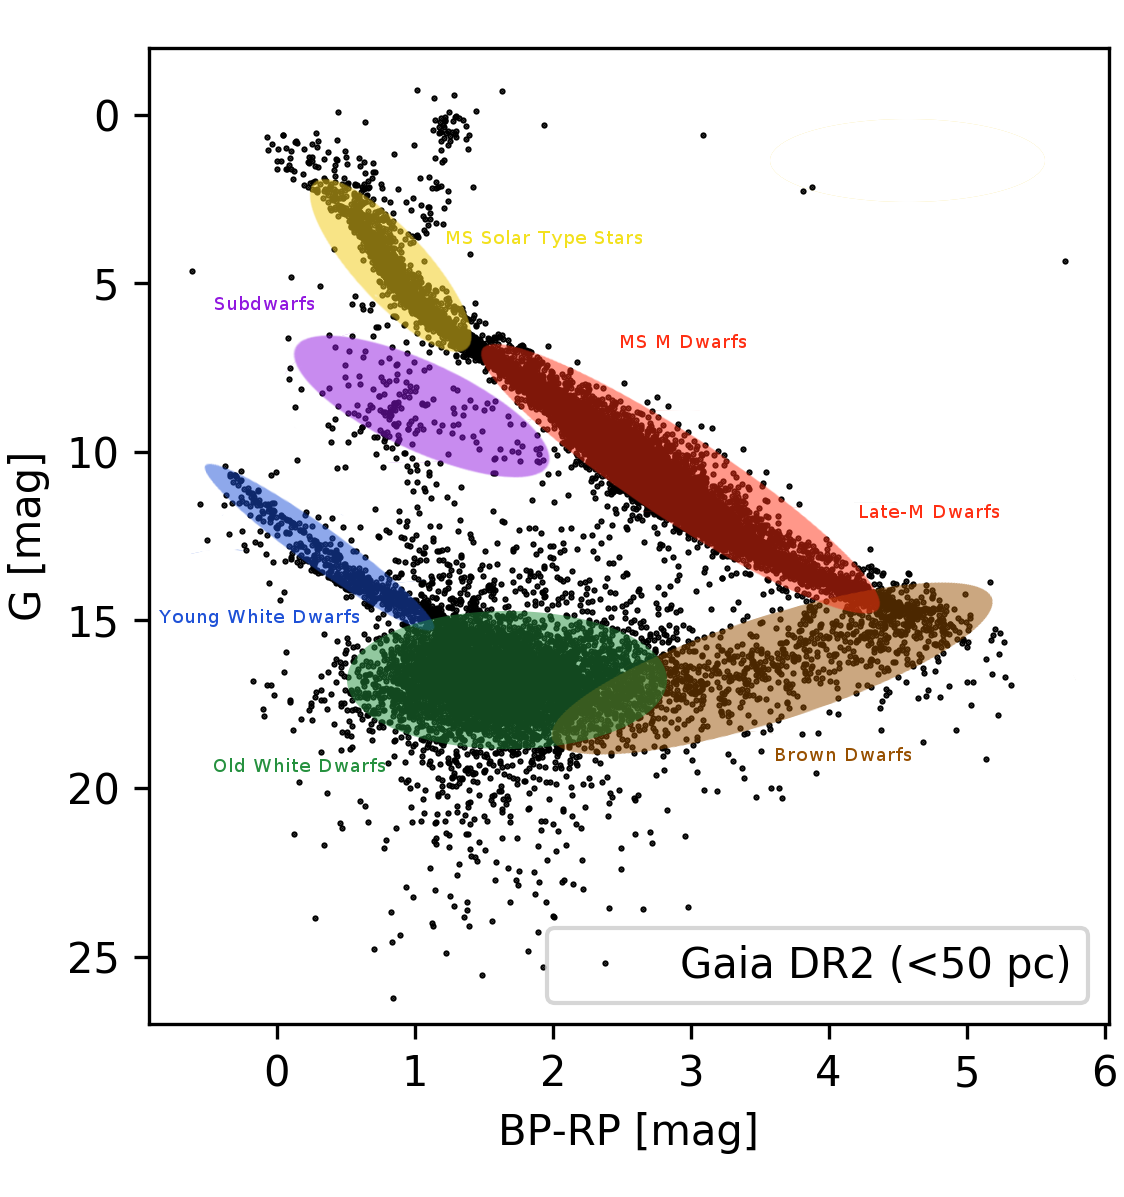
\includegraphics [scale=1.5] {gaia50types}
  \caption{На диаграмме <<показатель цвет $BP-RP$ -- абсолютная звездная величина в полосе G>> представлены звезды Gaia DR2 из ближайших окрестностей (до 50 пк). Цветными областями обозначено приблизительное разбиение звезд на группы, исходя из значений их показателей цвета и абсолютных звездных величин.}
  \label{fig:typ}
\end{figure}

\begin{figure}[pt]
  \centering
  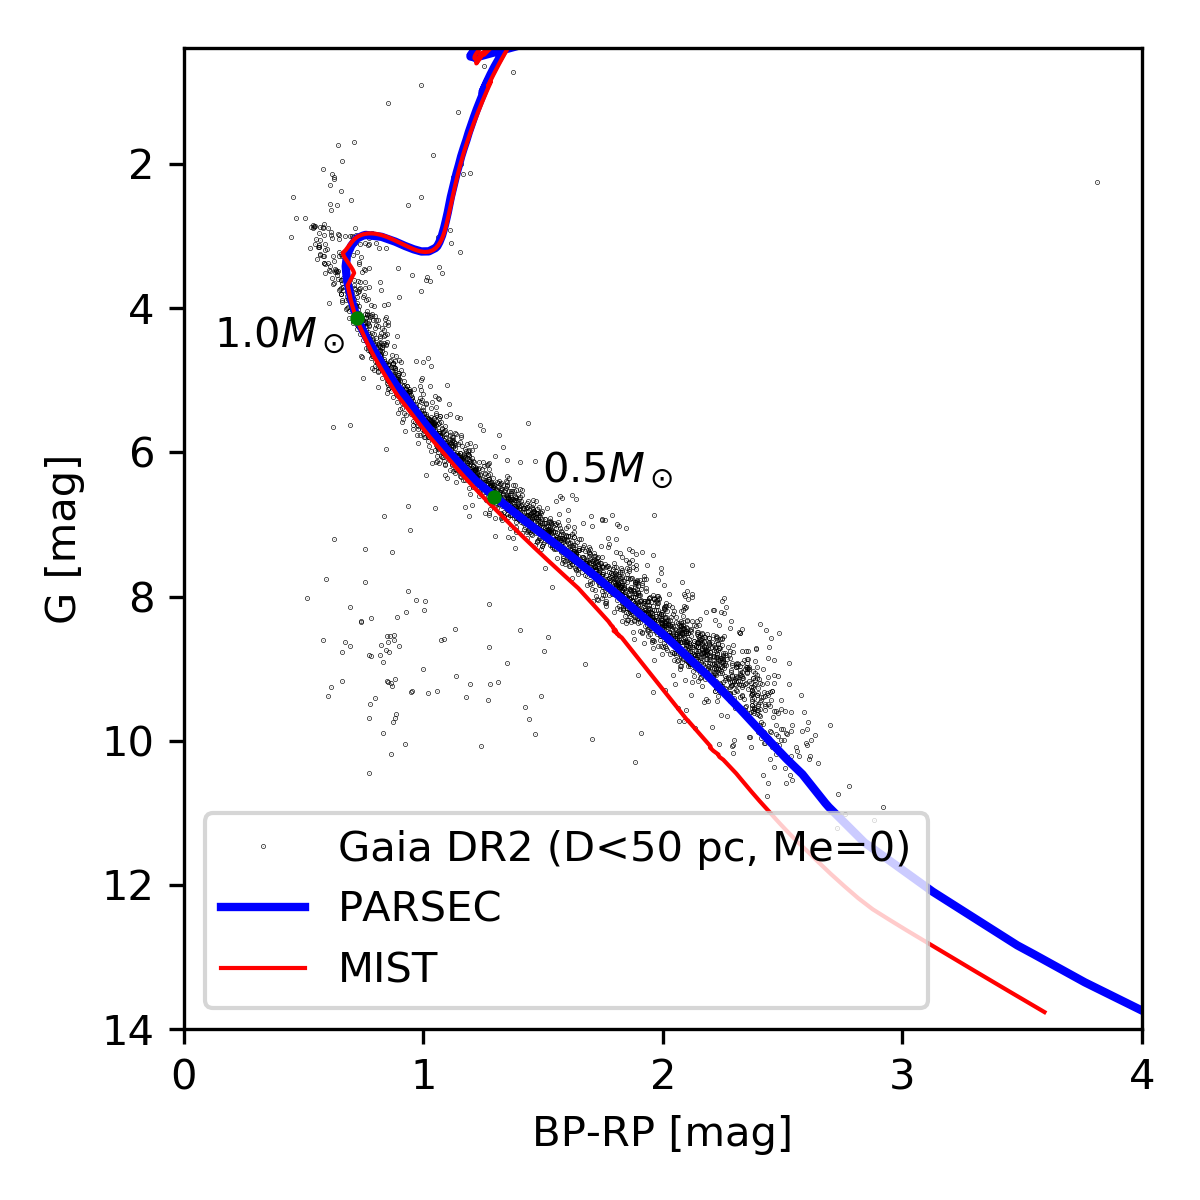
\includegraphics [scale=1.5] {parsec-mist-gaia}
  \caption{На диаграмме <<показатель цвет $BP-RP$ -- абсолютная звездная величина в полосе G>> представлены звезды Gaia DR2 из ближайших окрестностей (до 50 пк) с солнечной металличностью, соответствующие модельные изохроны проектов PARSEC и MIST, а также положения соответствующих звезд с массами 1 \(\textup{M}_\odot\) и 0.5 \(\textup{M}_\odot\).}
  \label{fig:iso}
\end{figure}

В настоящее время существует ряд проектов, нацеленных на конструирование моделей звезд различных типов. На рисунке~\ref{fig:iso} представлено сравнение звезд солнечной металличности из ближайших 50 пк по данным Gaia DR2 c модельными изохронами, построенными с помощью систем MIST \cite{2016ApJ...823..102C} и PARSEC \cite{2012MNRAS.427..127B}. Как видно из рисунка, для масс от 1 до 0.5 \(\textup{M}_\odot\) наблюдаемые данные очень хорошо согласуются с обеими изохронами, при массах менее 0.5 \(\textup{M}_\odot\) расхождение между системами изохрон весьма значительно, причем наилучшее согласие с наблюдениями имеет кривая, построенная с помощью PARSEC. Это можно объяснить в большей степени эмпирическим характером построения той части модели, которая описывает менее массивные звезды. Авторы PARSEC отмечают, что такой подход прежде всего связан с трудностью моделирования звездных атмосфер у объектов с сильным влиянием конвекционных процессов. Чтобы справиться с проблемой моделирования объектов легче, авторы PARSEC вносили поправки на основе данных для пары сотен наблюдаемых затменно-двойных звезд, для которых есть хорошие кривые лучевых скоростей (см. рисунок~\ref{fig:mrr}). Однако, выяснилось, что наблюдаемые затменно-двойные звезды слишком тесные, и соотношение масса-радиус для таких звезд не отвечает моделям одиночных звезд. Одно из предположений заключается в том, что в таких системах происходит инфляция радиуса за счёт взаимного нагрева компонент. Однако, попытка оценить такое влияние показала увеличение радиуса не более, чем на 6\,\%  при превосходстве светимости <<влияющего>> компаньона более, чем в 500 раз (см. рисунок~\ref{fig:inf}). Но эта работа продемонстрировала сложность физики взаимодействий в тесной системе маломассивных карликов, где имеют место  взаимные приливные деформации компонент. Поэтому крайне интересны двойные системы, состоящие из маломассивных звезд и при этом достаточно удаленные друг от друга, чтобы зависимость <<масса -- радиус>> соответствовала одиночным звездам. Собственно поиск таких систем и есть одна из целей настоящего исследования.

\begin{figure}[pt]
  \begin{minipage}[ht]{1\linewidth}\centering
    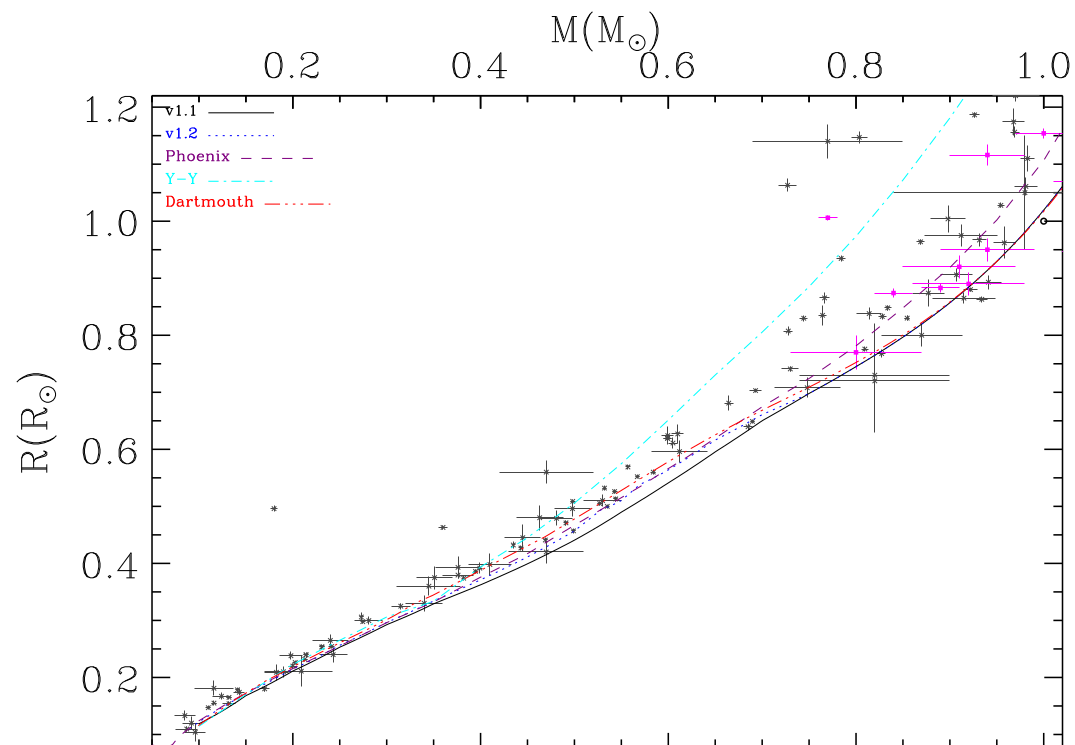
\includegraphics[width=0.8\linewidth]{parsecMRL1}% \\ а)
  \end{minipage}
  \hfill
  \begin{minipage}[ht]{1\linewidth}\centering
    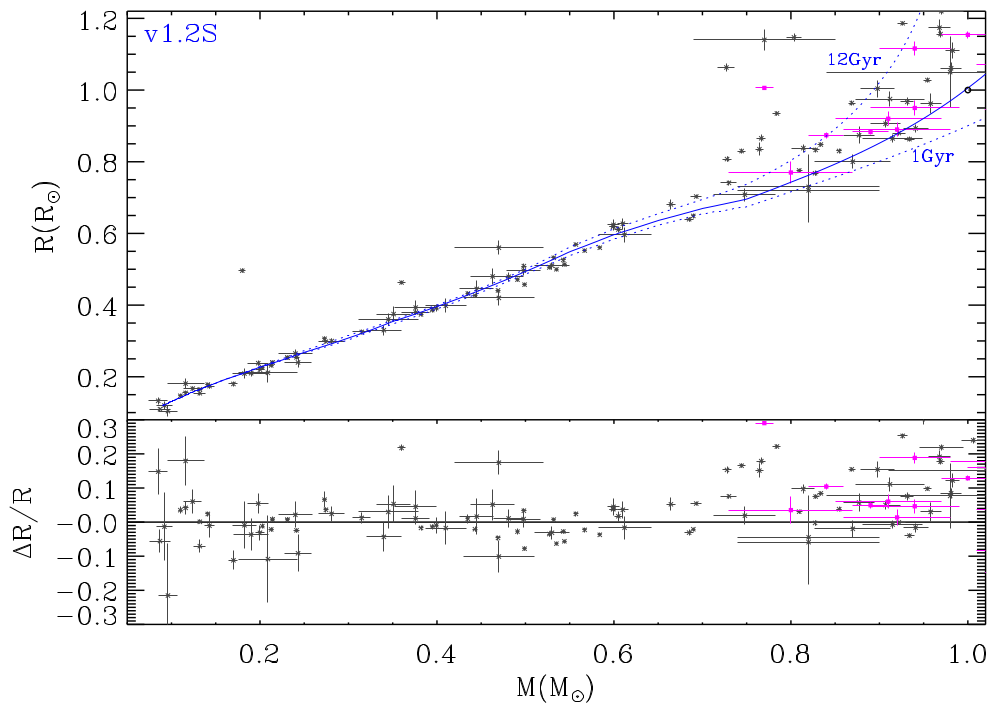
\includegraphics[width=0.8\linewidth]{parsecMRL2}% \\ б)
  \end{minipage}
  \caption{Сверху: эмпирическое отношение <<масса -- радиус>> для звезд с малой массой в солнечной окрестности. Черные звездочки "--- это двойные звезды; пурпурные квадраты "--- одиночные звезды. v1.1 и v1.2 "--- версии изохрон PARSEC (версия 1.2 "--- уточненная при помощи наблюдений нескольких сотен затменно-двойных, для которых есть хорошие кривые лучевых скоростей). Снизу: то же, только построенное для откалиброванного отношения <<T -- $\tau$>> (T "--- температура, $\tau$ "--- средняя оптическая глубина Росселанда) и с добавление изохрон для возрастов 1Gyr и 12Gyr. Взято из \cite{2014MNRAS.444.2525C}, рис. 2 и рис. 12).}
  \label{fig:mrr}
\end{figure}

\begin{figure}[pt]
  \centering
  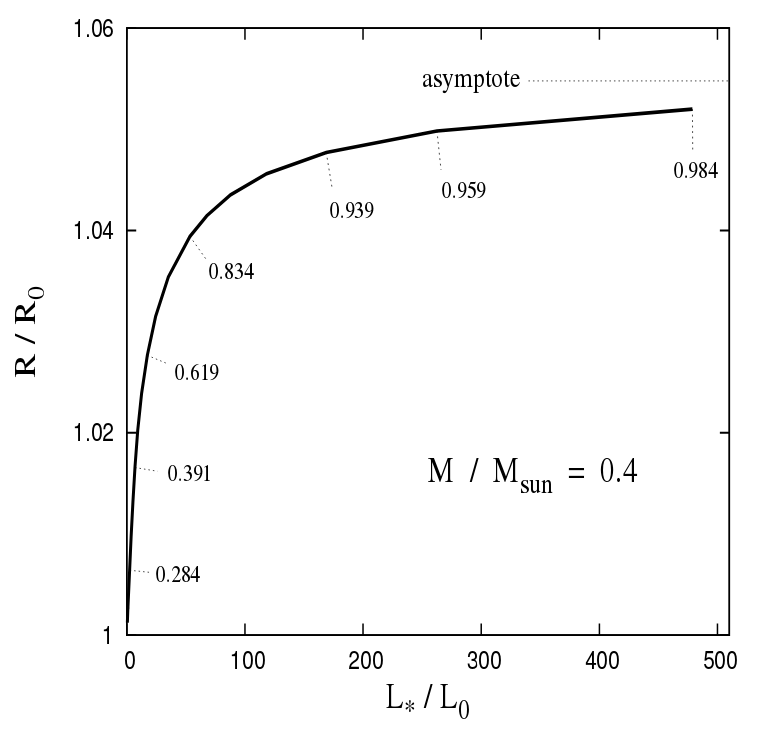
\includegraphics [scale=0.55] {radiusInflationLMSbinary}
  \caption{Попытка оценить влияние <<точечной>> компоненты затменно-двойной (a = 3 \(\textup{R}_0\)) со светимостью \(\textup{L}_*\) (отсечками на кривой показаны значения болометрического альбедо). Взято из \cite{2017A&A...601A..75L}, рис. 4.}
  \label{fig:inf}
\end{figure}

В качестве примера попытки построения эмпирической зависимости <<масса -- светимость>> (MLR) можно отметить работу \cite{2018MNRAS.479.5491E}, где использовались наблюдения звезд с наиболее надежными массами и светимостями. Всего в работу вошло 55 маломассивных объектов. На рисунке~\ref{fig:mlr} представлено сравнение этой модели с аналогичными кривыми по данным MIST и PARSEC, и как можно заметить, модели начинают расходиться при светимости меньше, а  объекты, наблюдаемые в пулковской программе изучения визуально-двойных звезд \cite{2018RAA....18...94S}, лежат у границ погрешностей эмпирической зависимости из работы \cite{2018MNRAS.479.5491E}, обозначенных пунктирной линией. Это тоже указывает на наличие дефицита надежных масс для звезд   M < 0.7~\(\textup{M}_\odot\). Поэтому калибровка существующих моделей карликовых звезд привязана к тесным системам, где оценки M и L могут быть искажены упомянутыми выше систематическими эффектами (несферичность, взаимный нагрев).

\begin{figure}[pt]
  \centering
  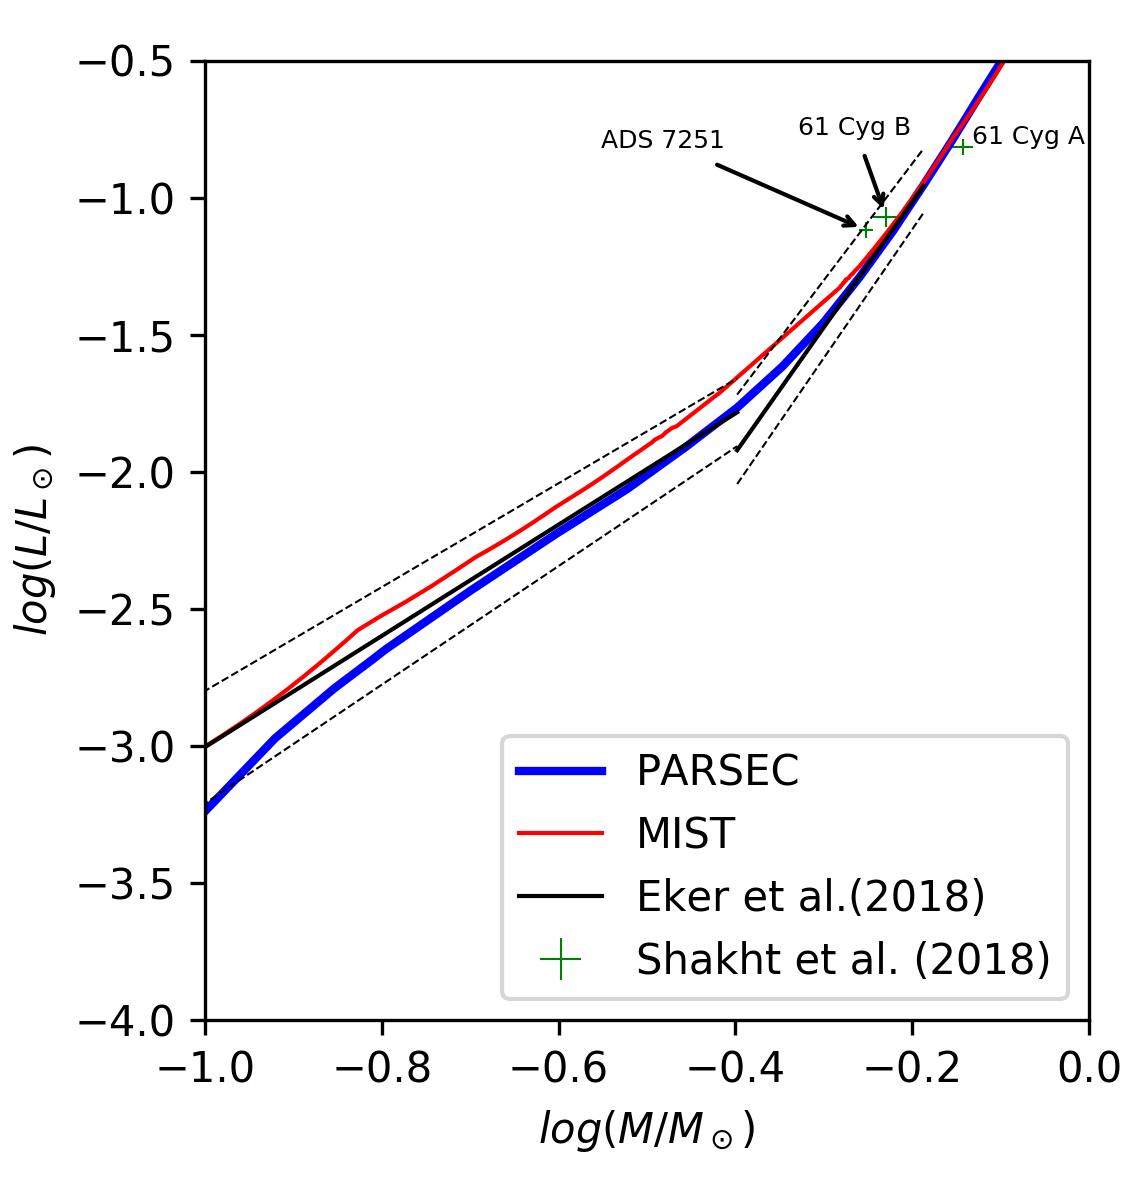
\includegraphics [scale=1.5] {mass-lum}
  \caption{Эмпирическая модель MLR \cite{2018MNRAS.479.5491E} (пунктиром обозначена граница ошибок модели), а также  аналогичные модели проектов PARSEC и MIST. Крестами обозначены визуально-двойные звезды из пулковской программы \cite{2018RAA....18...94S}.}
  \label{fig:mlr}
\end{figure}

Затронутая выше проблема учета конвекционных процессов в маломассивных звездах отмечается и в других работах. Например, в <<Обзоре маломассивных звезд и коричневых карликов>> \cite{2005astro.ph..9798C} говорится о сложности фотометрии звезд класса M5 и более поздних как раз из-за образования на поверхности большого числа звездных пятен и роста видимой активности диска и короны. Авторы объясняют это тем, что конвекция у таких объектов может распространяться вплоть до ядра.  Вообще, в данной работе говорится о целом наборе проблем, связанных с недостатком информации о карликах при их моделировании. На рисунке~\ref{fig:MLch} продемонстрировано, насколько хорошо существующие теоретические зависимости <<масса "--- абсолютная звездная величина>> согласуются с наблюдениями в оптическом диапазоне.

\begin{figure}[pt]
  \centering
  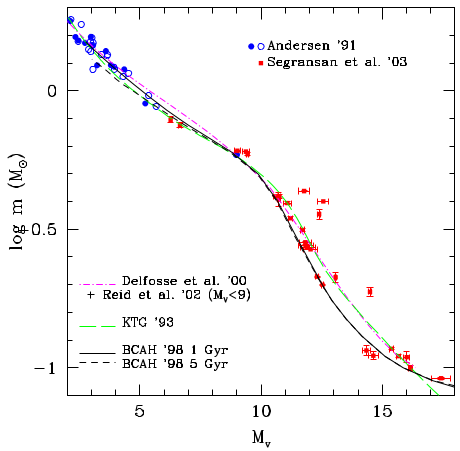
\includegraphics [scale=1.3] {chabrier-et-al-2005-3}
  \caption{Согласие теоретических моделей аналога зависимости <<масса -- звёздная величина>> с наблюдаемыми данными. Заметно расхождение теорий и наблюдений для звезд слабее 10 звездной величины и легче $\approx 0.5$\,\(\textup{M}_\odot\) (этому значению примерно соответствует отсчёт по вертикальной шкале около $-0.3$). Взято из \cite{2005astro.ph..9798C}, рис. 3.}
  \label{fig:MLch}
\end{figure}

Как можно заметить, для звёзд до \(\textup{10}^m\) согласие достаточно хорошее, тогда как более слабые объекты по диаграмме распределены несколько более хаотично и сильнее отклоняются от гладких модельных кривых. В статье говорится, что, вероятно, это связано с образованием большого количество линий поглощения. Исследователи отмечают, что в атмосферах маломассивных звёзд и коричневых карликов образуется множество молекул, чьи конденсаты и частицы сильно влияют на тепловую непрозрачность этих атмосфер. Излучение молекул часто поглощается в оптическом диапазоне или слишком слабо из-за эффекта обратного нагрева верхних слоев, где линии формируются. Всё это приводит к видимому покраснению звёзд, в частности, коричневые карлики излучают до 90\,\% своей энергии в ИК полосах, и авторы называют наиболее перспективными исследования данных объектов именно в этом диапазоне. Что согласуется с выводами авторов работы <<Необходимость инфракрасной астрометрии коричневых карликов в эпоху после Gaia>> \cite{2019BAAS...51c.105K}, которые указали на сложности наблюдений Gaia таких объектов. Исследователи отмечают, что диапазон наблюдений Gaia: $\lambda$ < 1,05 мкм \cite{2016A&A...595A...1G}, поэтому подавляющее большинство коричневых карликов, чьи спектры достигают максимума в ИК, не могут быть обнаружены. Например, в ближайших 20 парсеках Gaia может полностью исследовать только типы до L5 \cite{2019ApJS..240...19K}. И в материалах доклада проиллюстрирована необходимость астрометрического мониторинга на более длинных инфракрасных волнах.

Проблема надежного определения радиусов звёзд также упоминается в работе Шабрие \cite{2005astro.ph..9798C}. Отмечается, что используемые сейчас методы определения радиусов могут давать результаты, сильно отличающиеся друг от друга. Значения радиусов, определяемые через оценку наклона кривой блеска у затменных двойных получаются в среднем в 2 раза больше аналогичных радиусов, определенных высокоточной интерферометрией или через эффект гравитационного линзирования. Как уже отмечалось выше, это может быть связано с эффектом взаимного нагрева компонент слишком тесных систем.

Имеет смысл упомянуть об исследованиях по построению и интерпретации функции масс в окрестностях границы <<звёзды -- коричневые карлики>> \cite{2015ApJ...800...72T}. Здесь серьезное внимание уделяется проблеме адекватной оценки доли двойных систем для объектов малых масс. Функция масс претерпевает значимые изменения при разных значениях этой величины.  Это делает весьма актуальной задачу построения полной выборки двойных и кратных звезд в области малых масс. Наша работа имеет целью достичь продвижения в данном направлении.

Резюмируя вышеизложенное, естественно сделать вывод об актуальности исследования различных типов двойных и кратных систем карликовых звезд, в том числе "--- более широких, порядок периодов которых с одной стороны позволяет строить взаимные орбиты по высокоточным длительным наблюдениям, а с другой стороны "--- пространственное разделение компонент позволяло бы рассматривать каждую из компонент как одиночную звезду, без значительного влияния компаньона (большие полуоси у таких систем составляют порядка 10 а.е.). В современной научной печати можно найти многочисленные примеры работ, посвященных поиску двойных систем, разделению компонент и построению орбит двойных систем  (см., например, \cite{2015csss...18..805C}, \cite{2016ApJ...819...17O}).  

Построение численных моделей процесса звездообразования и дальнейшей динамической эволюции звездной популяции из молекулярных облаков позволяет получить модельные распределения доли двойных систем в зависимости от массы, отношения масс компонент и металличности, проанализировать различные распределения по орбитальным параметрам. Сопоставление результатов таких вычислений с наблюдениями затруднено неполнотой выборки для двойных систем, содержащих маломассивные компоненты. Это является еще одним обоснованием актуальности любых наблюдательных работ, направленных на поиск и изучение двойных и кратных систем среди карликовых звезд.

Сейчас можно найти немало исследований, посвященных построению численных сценариев звездообразования. Например, в работе \cite{2019MNRAS.484.2341B} представлен пример симуляции процесса формирования звездного скопления. Здесь учитывается масса факторов и явлений: химический состав межзвездной среды, влияние космических лучей, нагрев газа и пыли из-за излучения звезд, процессы диффузии и переноса излучения. В итоге модельное облако M = 500 \(\textup{M}_\odot\) порождает порядка сотни звезд суммарной массы $\approx$\,100~\(\textup{M}_\odot\) с медианной массой 0,15 \(\textup{M}_\odot\). Как видно из рисунка~\ref{fig:imf}, получившаяся функция масс наилучшим образом согласуется с результатами построения IMF \cite{2005ASSL..327...41C}, собравшим наблюдения маломассивных звезд и коричневых карликов на протяжении 50 лет.  Особое место в исследовании отведено изучению доли и свойств кратных объектов. Как следует из рисунка~\ref{fig:fract}, доля кратных систем в получившейся модели растёт с увеличением начальных масс объектов, и этот результат подтверждают и эмпирические данные. Причем исследователи отмечают, что так как доля кратных систем имеет явную корреляцию с значениями начальных масс, то при сравнении моделирования с наблюдениями всегда стоит использовать аналогичные диапазоны масс. На рисунке~\ref{fig:hist} представлено сравнение получившейся гистограммы распределения двойных, тройных и четверных систем по большим полуосям (тройные системы дают два значения полуосей, а четверные "--- три) с двумя эмпирическими построениями: для M-карликов и звезд с начальными массами солнечного типа. Отмечается, что поскольку большинство моделируемых объектов имеют малую массу, то ожидается, что распределение для M-карликов должно лучше соответствовать модели, и этот результат в большей мере воспроизводит гистограмма для двойных систем.  Попытка воссоздания эволюции доли двойных систем для кластеров звезд с различными начальными параметрами представлена, например, в работе \cite{2007ApJ...665..707H}. На рисунке~\ref{fig:evol} представлен результат моделирования эволюции доли двойных систем в кластере из 100~000 звезд, где в начальный заданный момент времени доля двойных составляла 10\,\%. Из рисунка видно, что с течением времени прогнозируемое моделью число кратных систем имеет явный тренд к возрастанию.

\begin{figure}[pt]
  \centering
  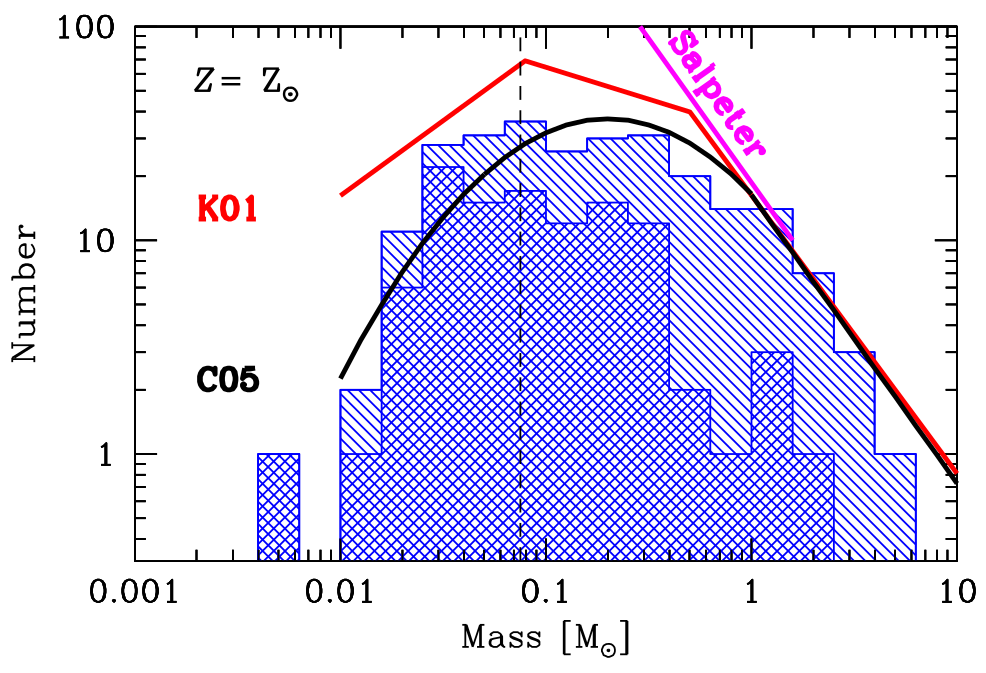
\includegraphics [scale=0.45] {Bate-IMF}
  \caption{Гистограмма IMF звезд и коричневых карликов солнечной металличности в рамках численной модели \cite{2019MNRAS.484.2341B}. Двойная штриховка "--- объекты без аккреции, одиночная штриховка "--- с аккрецией. Функции масс хорошо согласуются с данными \cite{2005ASSL..327...41C} (С05). Также представлены две другие IMF: Salpeter~\cite{1955ApJ...121..161S} и K01~\cite{2001MNRAS.322..231K}. Взято из \cite{2019MNRAS.484.2341B}, рис. 8, нижний левый.}
  \label{fig:imf}
\end{figure}

\begin{figure}[pt]
  \centering
  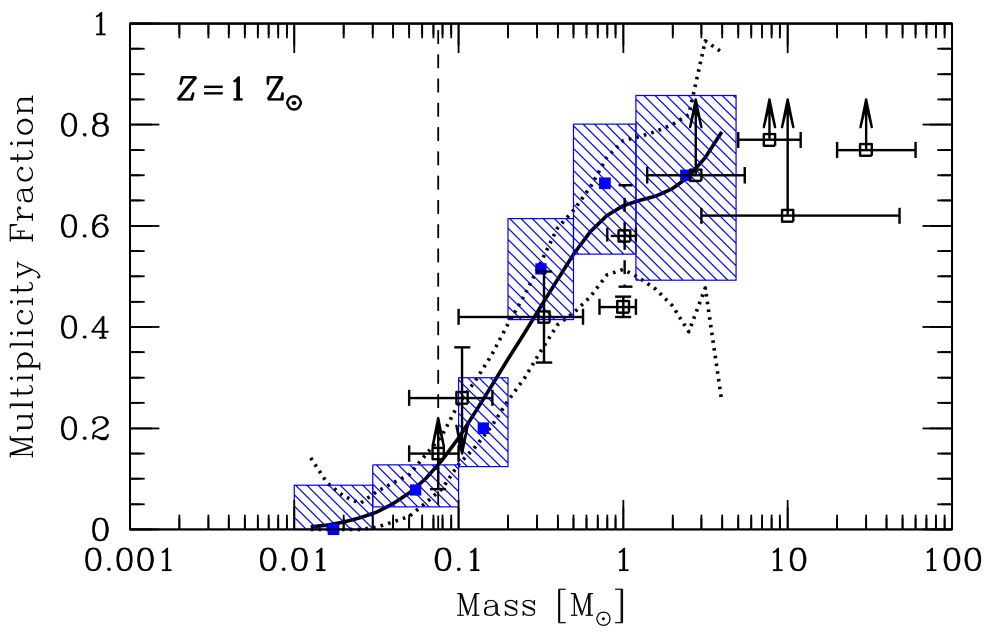
\includegraphics [scale=0.47] {Bate-BF}
  \caption{Доля кратности в зависимости от первичной массы звезд солнечной металличности в рамках численной модели \cite{2019MNRAS.484.2341B}. Синие закрашенные квадраты, окруженные заштрихованными областями, представляют результаты численных расчетов со статистической погрешностью 1$\sigma$. Толстая сплошная линия "--- кривая долей кратности, вычисленная с использованием скользящего логарифма, пунктирные линии "--- на 1$\sigma$-интервале вокруг нее. Незакрашенные квадраты с погрешностями и пределами "--- наблюдаемые доли кратных из исследований \cite{2003ApJ...587..407C}, \cite{2006AJ....132..663B}, \cite{1992ApJ...396..178F}, \cite{2010ApJS..190....1R}, \cite{1991A&A...248..485D}, \cite{2007A&A...474...77K}, \cite{2013MNRAS.436.1694R}, \cite{1999NewA....4..531P} и \cite{1998AJ....115..821M} слева направо.  Исследователи отмечают, что наблюдаемая тенденция увеличения кратности воспроизводится всеми рассмотренными расчетами, и поскольку доля кратных сильно зависит от начальных масс, важно, чтобы при сравнении моделей с наблюдениями использовались аналогичные массы. Взято из \cite{2019MNRAS.484.2341B}, рис. 10, нижний левый.}
  \label{fig:fract}
\end{figure}

\begin{figure}[pt]
  \centering
  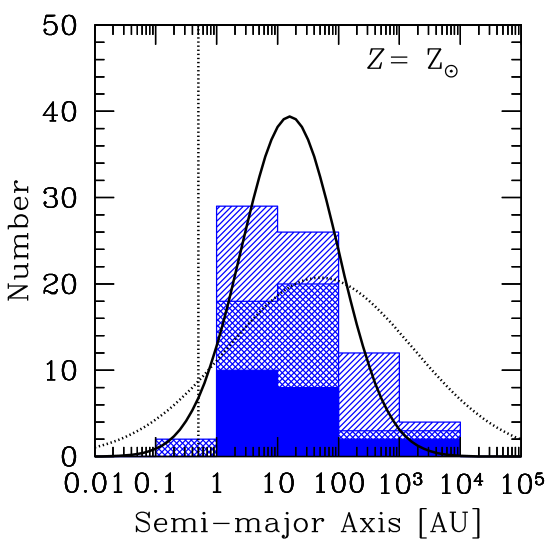
\includegraphics [scale=0.8] {Bate-a-distr}
  \caption{Гистограмма распределения кратных звезд солнечной металличности с начальными массами > 0.1Msun по большим полуосям в рамках численной модели \cite{2019MNRAS.484.2341B}.  Бары с одиночной, двойной и сплошной штриховкой представляют двойные, тройные и четверные системы соответственно. Сплошная кривая "--- распределение M-карликов из обзора \cite{2012ApJ...754...44J}, а пунктирная "--- распределение звезд с начальными массами солнечного типа из обзора \cite{2010ApJS..190....1R}. Поскольку большинство моделируемых систем имеют малую массу, ожидается, что распределение \cite{2012ApJ...754...44J} будет соответствовать лучше, чем \cite{2010ApJS..190....1R}. Вертикальная пунктирная линия показывает предел разрешающей способности расчетов, который определяется радиусами аккреции поглощающих частиц (0,5 а.е.). Взято из \cite{2019MNRAS.484.2341B}, рис. 11, третий слева.}
  \label{fig:hist}
\end{figure}


\begin{figure}[pt]
  \centering
  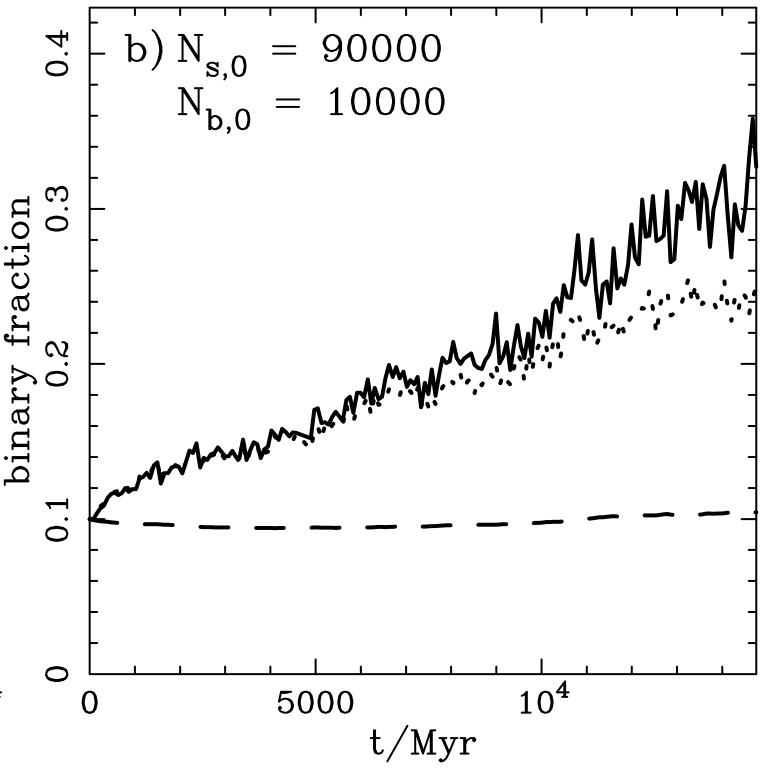
\includegraphics [scale=0.5] {Hurley}
  \caption{Эволюция доли двойных систем в ядре (сплошная линия), в пределах 10\,\% радиуса Лагранжа (пунктирная линия) и для всего кластера (пунктирная линия) в одной из моделей. $N_{s,0}$, $N{b,0}$ "---  количества одинарных и двойных звезд соответственно в исходной модели.  Взято из \cite{2007ApJ...665..707H}, рис. 7b.}
  \label{fig:evol}
\end{figure}

Однако, пока сложно утверждать, что даже совокупность существующих обзоров и программ решает проблему в полной мере. К сожалению, несмотря на существенный прогресс в исследовании кратных систем, который дает Gaia DR2, даже после значительного исправления первого релиза, данные миссии также не дают полноты выборки для визуальных двойных звезд с разделением $\rho$ менее $2''$ (рисунок~\ref{fig:compl}), что отмечают и авторы \cite{2018A&A...616A..17A},\cite{2018A&A...616A...2L}. Это может быть связано со сложностью анализа изображения тесных систем в Gaia DR2 \cite{2016A&A...595A...3F}, когда FWHM (ширина на полувысоте) становится меньше углового разделения $\rho$ (см. рисунок~\ref{fig:spf}). Сложность разделения тесных систем сказывается и на ошибках определения пиксельных координат, что в свою очередь влияет на вычисляемые значения собственных движений и параллаксов. Например, на рисунке~\ref{fig:err} можно увидеть, как относительная точность параллаксов Gaia DR2 падает при $\rho$~<~$2''$. Кроме того, отмечается проблема кросс-идентификации быстрых объектов ($\mu$~>~100 mas/yr), которые в основном как раз относятся к ближайшему звездному населению. Как указано в GaiaDR2 Documentation 1.2\footnote{\textit{https://gea.esac.esa.int/archive/documentation/GDR2/index.html}}, для звезд с разделением менее $0.7''$ всегда будет стоять проблема кросс-идентификации, и поэтому объекты Gaia DR2 с флагом <<duplicate source>> предлагается отдельно проверять, являются ли они действительно дубликатами одиночной звезды или же входят в двойную или кратную систему. Помимо проблемы отождествления тесных объектов, стоит упомянуть, что период наблюдений миссии Gaia строго ограничен и не дает возможности получения достаточного количества наблюдений для построения орбит широких пар, периоды взаимного обращения которых сильно превалируют над сроком жизни космического аппарата.

\begin{figure}[pt]
  \centering
  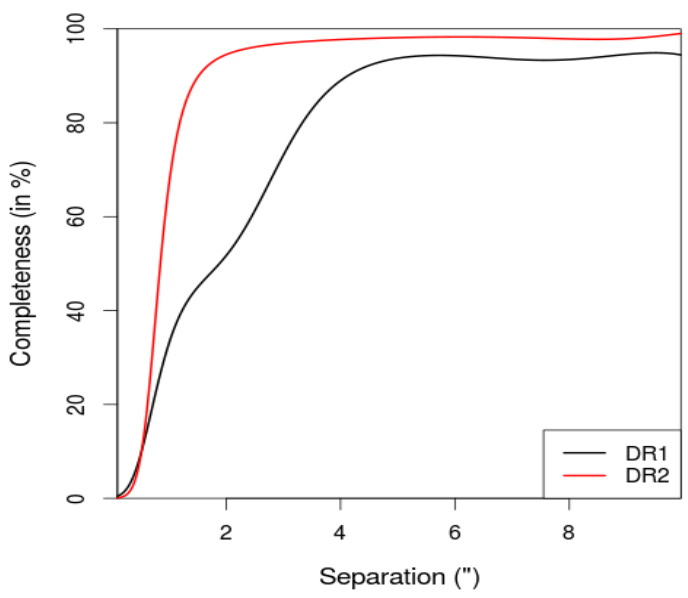
\includegraphics [scale=0.6] {gaia-complitness-for-binaries}
  \caption{Полнота (\%) визуальных двойных звёзд из каталога WDS в зависимости от разделения между компонентами (WDS), детектируемых в ходе миссии Gaia.  Gaia DR1 (черный), Gaia DR2 (красный). Заметно снижение полноты выборки двойных для тесных систем ($\rho$ < 2 arcsec). Взято из \cite{2018A&A...616A..17A}, рис. 8.}
  \label{fig:compl}
\end{figure}

\begin{figure}[pt]
  \centering
  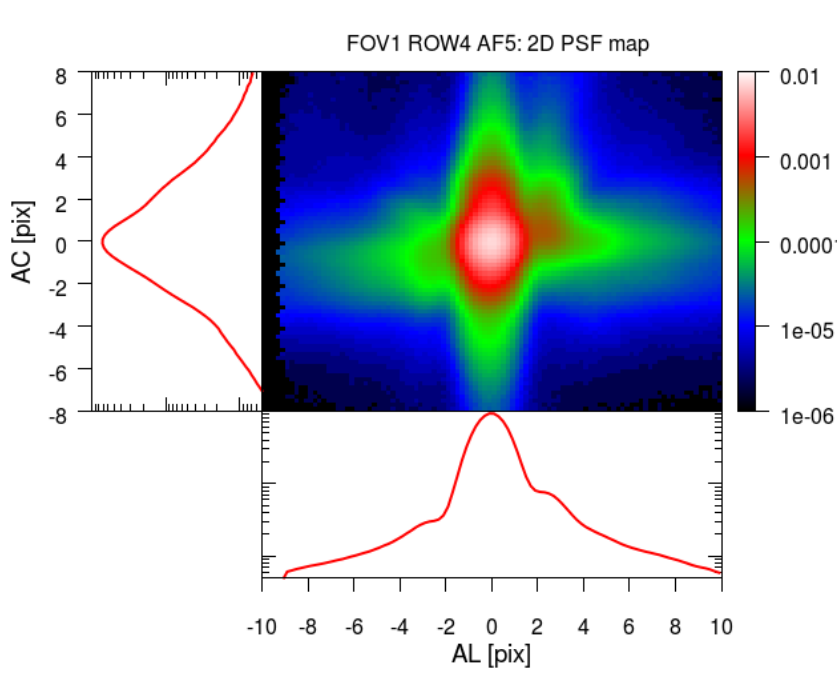
\includegraphics [scale=0.6] {gaia-psf}
  \caption{PSF изображения тесной двойной (1.2$''$ на 2.8$''$) демонстрирует сложность разделения в Gaia DR2 изображений подобных звезд. Взято из \cite{2016A&A...595A...3F},  рис. 7.}
  \label{fig:spf}
\end{figure}

\begin{figure}[pt]
  \centering
  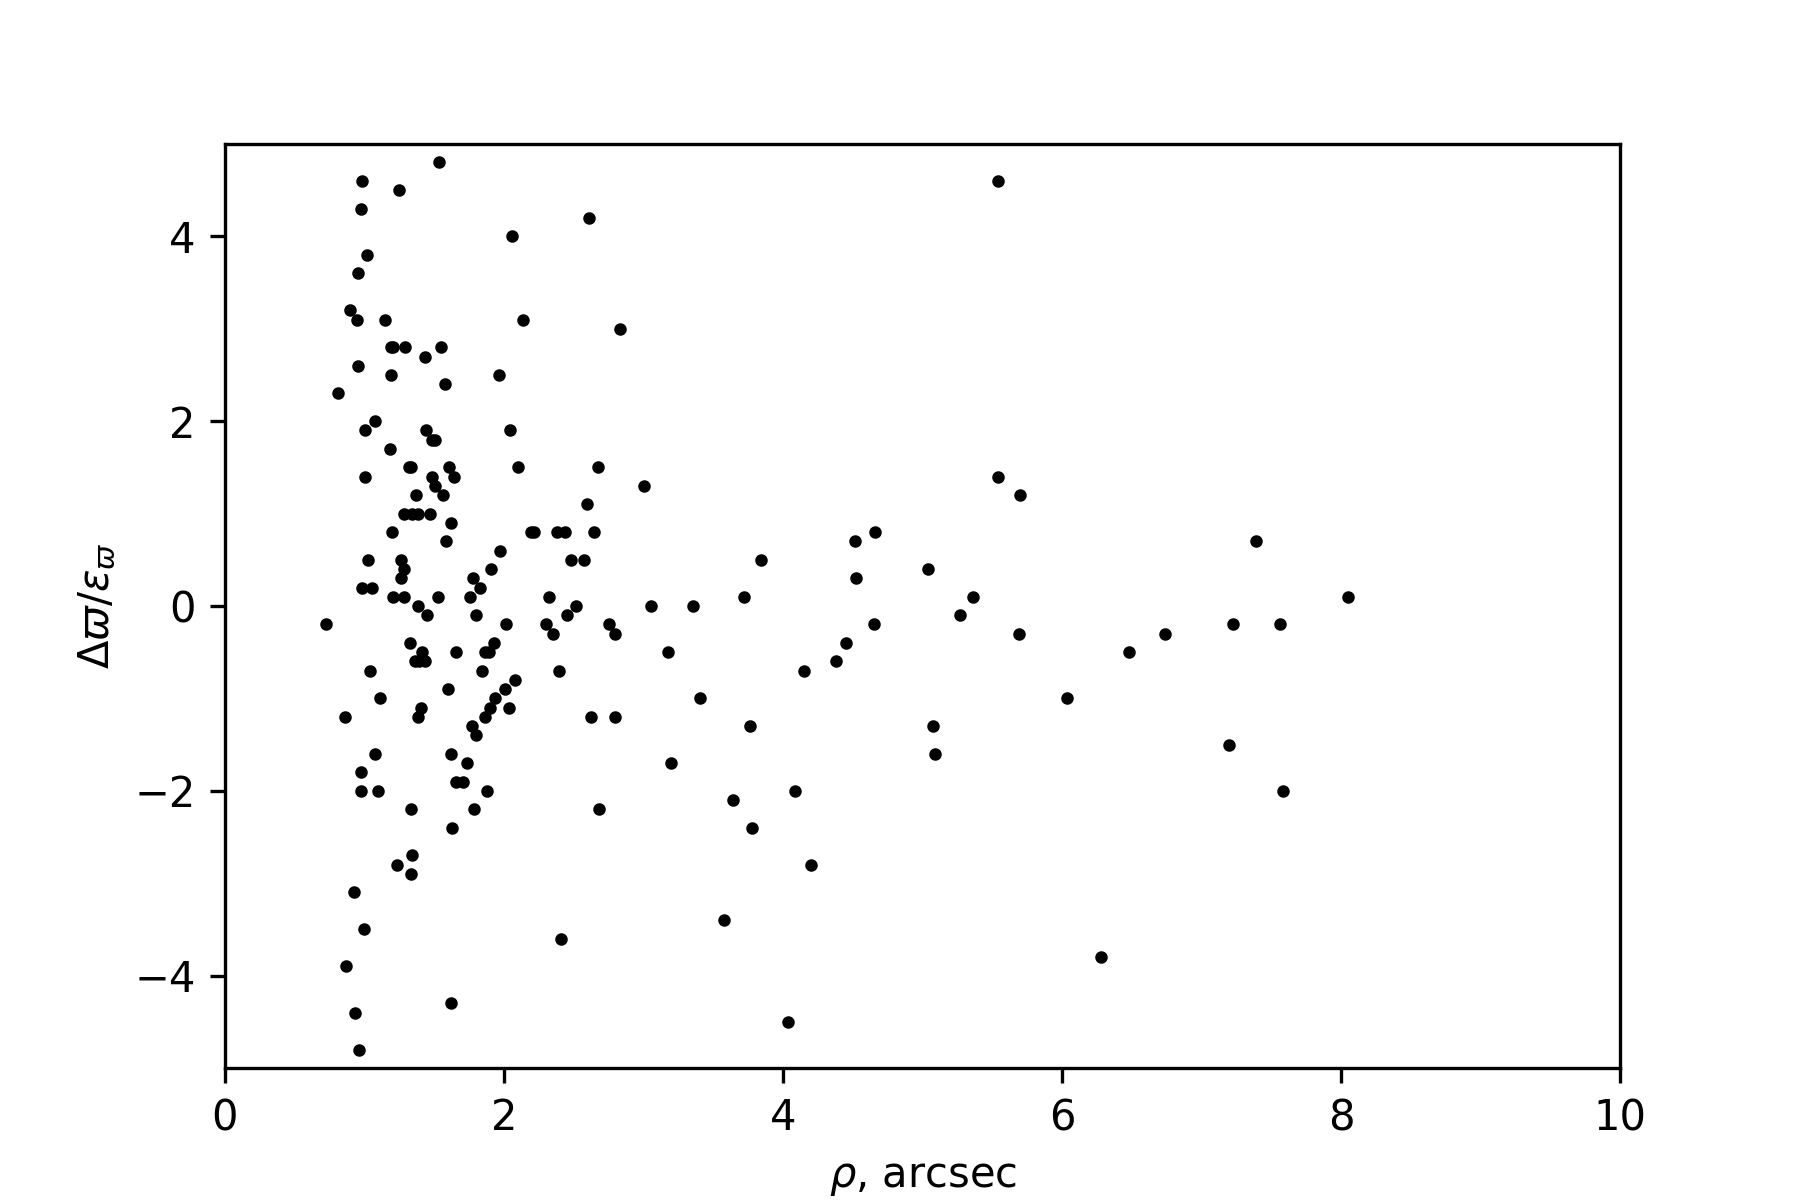
\includegraphics [scale=1.2] {delta_pi-vs-rho}
  \caption{Увеличение разброса относительных ошибок параллаксов Gaia для изображений звезд с разделением менее 3$''$ указывает на существенное снижение точности определения пиксельных координат компонент.}
  \label{fig:err}
\end{figure}

В связи с указанными проблемами важным становится применение всех доступных методик детектирования кратности звезд и использование по возможности всех доступных наблюдений звезд, охватывающих широкий диапазон эпох. Исследования звезд в ближайших 50 пк от Солнца дают возможность наиболее эффективного их применения. Как можно убедиться из рисунка~\ref{fig:sepdis}, для звездных систем с величинами больших полуосей порядка 10 а.е. видимое разделение компонент даже в ближайшем окружении составляет меньше $1''$. К счастью, существующие методы высокого разрешения (спекл-интерферометрия, метод удачных экспозиций) позволяют разделять объекты $\rho$~<~$1''$ (см. рисунок~\ref{fig:lucky}). Однако данные методы сложно применять массово, так как требуют таргетированных и часто многочисленных наблюдений, и больше подходят для построения орбит уже выявленных двойных и кратных систем.

\begin{figure}[pt]
  \centering
  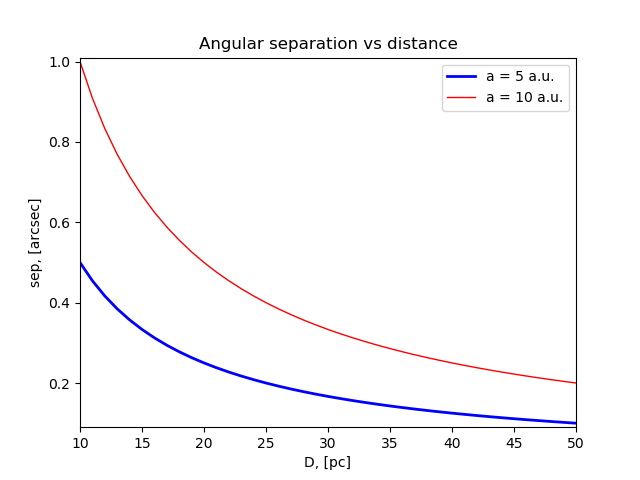
\includegraphics [scale=1.1] {separation-vs-distance}
  \caption{Представлена зависимость от удаления видимого углового разделения компонент систем с заданными большими полуосями. Поиск и определение динамических параметров маломассивных двойных систем "--- актуальная задача, требующая наблюдений широкого класса объектов, для которых разделение $\rho$~<~FWHM.}
  \label{fig:sepdis}
\end{figure}

\begin{figure}[pt]
  \centering
  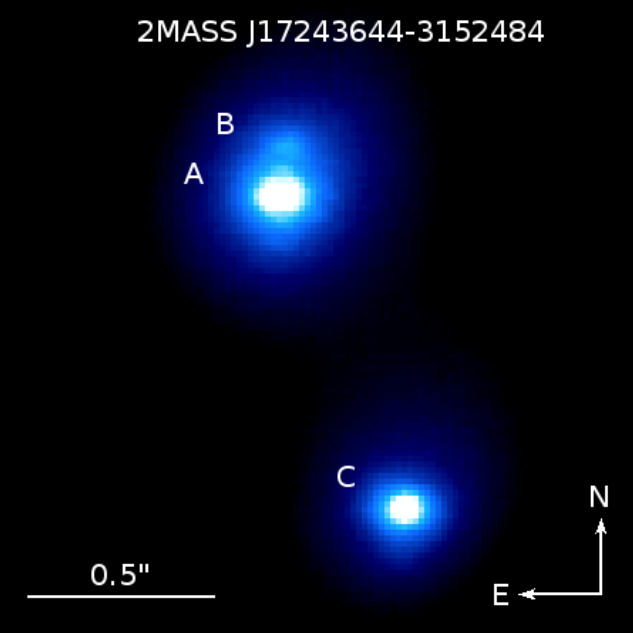
\includegraphics [scale=0.6] {lucky-imaging-example}
  \caption{Рис 15. 3.5m New Technology Telescope (NTT) "--- метод удачных экспозиций (Lucky imaging). Взято из \cite{2017A&A...599A..70J}, рис. 1. }
  \label{fig:lucky}
\end{figure}

Близость исследуемых объектов позволяют эффективно применять различные методы современной астрономии для их изучения. Например, наиболее заметные смещения компонент близких систем по лучу зрения дают возможность плодотворно выявлять оптически неразрешаемые спектрально-двойные звезды благодаря значительному проявлению эффекта доплеровского смещения спектральных линий. Однако, объектами таких исследований становятся в основном всё те же тесные системы, массы и радиусы которых сложно использовать для построения моделей одиночных звезд.

Целью данной работы является разработка метода поиска двойных и кратных звезд, дальнейшее определение орбитальных параметров которых позволят получить более надежные массы, радиусы и светимости маломассивных звезд и коричневых карликов и уточнить фундаментальные закономерности для этих групп объектов. Исследуемые системы преимущественно должны быть не слишком тесными, чтобы компоненты не влияли в значительной мере на характеристики друг друга, а их периоды составляли несколько десятилетий, что дает возможность построить орбиту по короткой дуге за относительно небольшой отрезок времени. Поэтому объектами наших поисков являются двойные звезды низкой светимости из ближайшего окружения Солнца, большие полуоси взаимных орбит которых составляют примерно 5--10 а.е.. Как уже отмечалось, даже в ближайшей солнечной окрестности такие системы часто разрешимы только  с помощью наблюдений методами высокого разрешения  (спекл-интерферометрия, метод удачных экспозиций), которые нельзя использовать для массовых наблюдений. Поэтому одна из задач данного исследования состоит в разработке методов обнаружения искомых двойных систем, основанных на подходах традиционной наземной оптической астрометрии и анализа изображений.

Актуальность рассматриваемых проблем способствовала тому, что в XX в. было реализовано несколько проектов, направленных на обнаружение быстрых звезд \cite{1955AJ.....60..274D}, \cite{1979nlcs.book.....L} и на определение их собственных движений и тригонометрических параллаксов \cite{1995gcts.book.....V}. Научные группы из различных обсерваторий прилагают усилия в этом направлении. Большой цикл работ по данной тематике представляет команда проекта RECONS (см., например, \cite{2017AJ....153...14W}), имеются существенные результаты в рамках проекта MEarth \cite{2017ApJ...836..124D}. Часть исследований в рамках пулковской программы по изучению звезд с большими собственными движениями имела целью детектирование двойных систем, о чем свидетельствует цикл работ: \cite{2011AstL...37..420K}, \cite{2015AstL...41..833K}, \cite{2016AstL...42..686K}.

\newpage

Подводя итог вводной части работы коротко резюмируем основные моменты.
% {\progress}
% Этот раздел должен быть отдельным структурным элементом по
% ГОСТ, но он, как правило, включается в описание актуальности
% темы. Нужен он отдельным структурынм элемементом или нет ---
% смотрите другие диссертации вашего совета, скорее всего не нужен.

{\aim} данной работы является выявление двойных систем среди близких к Солнцу маломассивных карликовых звезд. 

Для~достижения поставленной цели необходимо было решить следующие {\tasks}:
\begin{enumerate}
  \item Оценить полноту современных обзоров и списков двойных систем;
  \item Сформировать список звезд для исследования;
  \item Разработать методы быстрого и массового поиска двойных систем среди близких к Солнцу маломассивных карликов, основанных на подходах наземной оптической астрометрии и анализа цифровых изображений звездообразных объектов.
\end{enumerate}

Актуальность данного исследования обусловлена недостатком надежных оценок масс для карликовых звезд, затрудняющим построение их физических моделей с одной стороны, и необходимостью верификации численных моделей формирования звездных популяций, в которой важную роль играют эмпирические распределения двойных систем по ряду параметров, с другой стороны.

{\novelty}
\begin{enumerate}
  \item Были предложены новые варианты методик поиска двойных систем на основе анализа собственных движений и путем анализа формы изображений звезд на ПЗС-кадрах;
  \item Выполнены собственные ПЗС-наблюдения, позволившие произвести проверку адекватности разработанных методов и выявить 259 звезд-кандидатов в двойные системы;
  \item В результате спекл-интерферометрических наблюдений на БТА САО РАН и 2.5 м телескопе КГО ГАИШ МГУ впервые детектирована двойственность систем J1158+4239, J1135+0414, J1147+6050, независимо подтверждены ранее уже выявленные двойные звезды J1601+3714, J0259+3636.
\end{enumerate}

Теоретическая значимость работы определяется модификацией метода Вилена, позволяющей выявлять двойственность звезд на основе анализа собственных движений на основе ПЗС-кадров и сканов фотопластинок с общей системой опорных звезд; адаптацией шейплет-формализма для оценивания эллиптичности и асимметрии звездных изображений на ПЗС-кадрах.

{\influence} состоит в проведении большого цикла астрономических наблюдений на Нормальном астрографе и метровом телескопе «Сатурн» в Пулковской обсерватории, анализ результатов которого позволил выявить двойственность упомянутых выше звезд. Важно, что представленные методы реализованы в виде программного обеспечения, которое может быть адаптировано для других инструментов различных обсерваторий.

{\methods} За основу исследований были взяты зарекомендовавшие себя технологии исследования быстрых звезд ($\Delta\mu$-двойные) и анализа изображений (shapelet-декомпозиция), которые были адаптированы с учетом исследуемого материала и успешно применены для поиска двойных звезд среди близких карликов.

{\defpositions}
\begin{enumerate}
  \item Модификация метода Вилена по выявлению звезд-кандидатов в $\Delta\mu$-двойные;
  \item Адаптация шейплет-формализма для детектирования скрытых двойных звездных изображений;
  \item Выявление 259 звезд--кандидатов в маломассивные двойные системы;
  \item Подтверждение двойственности пяти систем методами высокого разрешения.
\end{enumerate}


{\reliability} полученных результатов обеспечивается частичным присутствием найденных двойных звезд в существующих каталогах двойных звезд, в том числе "--- WDS.


{\probation}
Детальное изложение методов и результатов работы представлено в четырех публикациях, индексируемых в наукометрических базах данных (web of science, Scopus и т.п.), в устных докладах на российских и международных конференциях (астрометрические конференции <<Пулково--2012>>, <<Пулково--2015>>, <<Пулково--2018>>; ВАК--2013 (Санкт-Петербург); ВАК--2016 (Нижний Архыз); <<Современная астрометрия>> (Москва)), астрометрических семинарах Пулковской обсерватории и Пулковских молодежных конференциях. Кроме того, результаты исследований доступны в астрономических базах данных (CDS, WDS).
%\textbf{Публикации.} Основные результаты по теме диссертации изложены в 4 печатных изданиях. Из них 3 изданы в журналах, рекомендованных ВАК, 4 индексируются в Scopus (1 работа является материалами конференции), 3 индексируются в Web of Science. 

{\contribution} Автор принимал активное участие во многих этапах работы: наблюдения на пулковских  телескопах (Нормальном астрографе и телескопе <<Сатурн>>), написание программного обеспечения для вычисления и анализа собственных движений звезд, написание текстов для совместных с соавторами научных статей, выступления на научных конференциях с устными докладами, посвященными настоящему исследованию. 


%\ifnumequal{\value{bibliosel}}{0}
{%%% Встроенная реализация с загрузкой файла через движок bibtex8. (При желании, внутри можно использовать обычные ссылки, наподобие `\cite{vakbib1,vakbib2}`).
    %{\publications}% Основные результаты по теме диссертации изложены в XX печатных изданиях,
    %X из которых изданы в журналах, рекомендованных ВАК,
    %X "--- в тезисах докладов.
}% 
{%%% Реализация пакетом biblatex через движок biber
    %\begin{refsection}[bl-authorvak,bl-authorwos,bl-authorscopus,bl-authorother,bl-authorconf]
        % Это refsection=1.
        % Процитированные здесь работы:
        %  * подсчитываются, для автоматического составления фразы "Основные результаты ..."
        %  * попадают в авторскую библиографию, при usefootcite==0 и стиле `\insertbiblioauthor` или `\insertbiblioauthorgrouped`
        %  * нумеруются там в зависимости от порядка команд `\printbibliography` в этом разделе. 
        %  * при использовании `\insertbiblioauthorgrouped`, порядок команд `\printbibliography` в нём должен быть тем же (см. biblio/biblatex.tex)
        %
        % Невидимый библиографический список для подсчёта количества публикаций:
        %\printbibliography[heading=nobibheading, section=1, env=countauthorvak,    keyword=biblioauthorvak]%
        %\printbibliography[heading=nobibheading, section=1, env=countauthorwos,    keyword=biblioauthorwos]%
        %\printbibliography[heading=nobibheading, section=1, env=countauthorscopus, keyword=biblioauthorscopus]%
        %\printbibliography[heading=nobibheading, section=1, env=countauthorconf,   keyword=biblioauthorconf]%
        %\printbibliography[heading=nobibheading, section=1, env=countauthorother,  keyword=biblioauthorother]%
        %\printbibliography[heading=nobibheading, section=1, env=countauthor,       keyword=biblioauthor]%
        %
        % Цитирования.
        %  * Порядок перечисления определяет порядок в библиографии (только внутри подраздела, если `\insertbiblioauthorgrouped`).
        %  * Если не соблюдать порядок "как для \printbibliography", нумерация в `\insertbiblioauthor` будет кривой.
        %  * Если цитировать каждый источник отдельной командой --- найти некоторые ошибки будет проще.
        %
        %% authorvak
        %\nocite{vakbib1}%
        %\nocite{vakbib2}%
        %\nocite{vakbib3}
        %
        %% authorwos
        %\nocite{wosbib1}%
        %
        %% authorscopus
        %\nocite{scbib1}%
        %
        %% authorconf
        %\nocite{confbib1}%
        %\nocite{confbib2}%
        %
        %% authorother
        %\nocite{bib1}%
        %\nocite{bib2}%
        %\nocite{bib3}
        %\nocite{bib4}
        %\nocite{bib5}
        %
        %
        %{\publications} Основные результаты по теме диссертации изложены в~\arabic{citeauthor}~печатных изданиях,
        %\newcounter{citeauthorscwostot}% сумма citeauthorscopus и citeauthorwos
        %\setcounter{citeauthorscwostot}{\value{citeauthorscopus}}%
        %\addtocounter{citeauthorscwostot}{\value{citeauthorwos}}%
        %\arabic{citeauthorvak} из которых изданы в журналах, рекомендованных ВАК\sloppy%
        %\ifnum \value{citeauthorscwostot}>0%
        %    , \arabic{citeauthorscwostot} "--- в~периодических научных журналах, индексируемых Web of Science и Scopus\sloppy%
        %\fi%
        %\ifnum \value{citeauthorconf}>0%
        %    , \arabic{citeauthorconf} "--- в~тезисах докладов.
        %\else%
        %    .
        %\fi
    %\end{refsection}%
    %\begin{refsection}[bl-authorvak,bl-authorwos,bl-authorscopus,bl-authorother,bl-authorconf]
        % Это refsection=2.
        % Процитированные здесь работы:
        %  * попадают в авторскую библиографию, при usefootcite==0 и стиле `\insertbiblioauthorimportant`.
        %  * ни на что не влияют в противном случае
        %\nocite{vakbib2}%vak
        %\nocite{bib1}%other
        %\nocite{confbib1}%conf
    %\end{refsection}%
	%
	% Всё, что вне этих двух refsection, это refsection=0,
	%  * для диссертации - это нормальные ссылки, попадающие в обычную библиографию
	%  * для автореферата:
	%     * при usefootcite==0, ссылка корректно сработает только для источника из `external.bib`. Для своих работ --- напечатает "[0]" (и даже Warning не вылезет).
	%     * при usefootcite==1, ссылка сработает нормально. В авторской библиографии будут только процитированные в refsection=0 работы.
}
 % Характеристика работы по структуре во введении и в автореферате не отличается (ГОСТ Р 7.0.11, пункты 5.3.1 и 9.2.1), потому её загружаем из одного и того же внешнего файла, предварительно задав форму выделения некоторым параметрам

\textbf{Объем и структура работы.} Диссертация состоит из~введения, трёх глав,
заключения и~двух приложений.
%% на случай ошибок оставляю исходный кусок на месте, закомментированным
%Полный объём диссертации составляет  \ref*{TotPages}~страницу
%с~\totalfigures{}~рисунками и~\totaltables{}~таблицами. Список литературы
%содержит \total{citenum}~наименований.
%
Полный объём диссертации составляет
\formbytotal{TotPages}{страниц}{у}{ы}{}, включая
\formbytotal{totalcount@figure}{рисун}{ок}{ка}{ков} и
\formbytotal{totalcount@table}{таблиц}{у}{ы}{}.   Список литературы содержит
\formbytotal{citenum}{наименован}{ие}{ия}{ий}.
    % Введение
\chapter{Астрометрический подход к поиску двойных систем} \label{ch:ch1}
\section{Исторический опыт астрометрического исследования быстрых звезд} \label{sec:ch1/sec1}
Развитие методов фотографической астрометрии на рубеже XIX--XX веков позволило начать массовое определение собственных движений звезд, не входящих в каталоги, построенные на основе меридианных наблюдений. Следствием этого стало открытие в 1916 году Эдвардом Барнардом звезды, с самым большим собственным движением \cite{1916AJ.....29..181B}. Сравнительно быстрое перемещение звезды Барнарда на фоне соседей ($\mu$~=~10.358~$''$/yr) закрепило за ней название <<летящей>>. Звезда Барнарда не является ближайшей к Солнцу, однако ожидаемо входит в наиболее тесное с нами звёздное соседство. Расстояние до <<летящей>> звезды чуть более 1.8~пк, и она является четвёртой известной звездой по мере удаления от Солнца, уступая в близости только системе звёзд Альфа Центравра. Однако, помимо выдающегося собственного движения, она имеет и значительную величину лучевой скорости, при этом приближаясь к Солнцу (\(\textup{М}_r\)~>~110 км/сек), и по оценкам может обогнать ближайшую к нам систему звёзд примерно к 11800 году. Стоит также отметить, что звезда Барнарда является красным карликом "--- представителем одной из наиболее многочисленных групп ближайшего околосолнечного населения Галактики. 

Значительные величины собственных движений звезд дают простор для приложения астрометрических методов поиска двойных и кратных объектов. Здесь на самом деле речь идет о весьма разнообразных подходах. Наиболее старый заключается в попытке обнаружить орбитальное движение для хорошо разрешаемых звездных пар. Эта задача вышла на передний план развития наблюдательной астрономии в конце XVIII века. В 1803 году в мемуарах Гершеля было впервые надежно показано наличие орбитального движения. Этот метод, в основном, касается широких пар с относительно большими периодами обращения (сотни и тысячи лет). Если иметь ввиду солнечную окрестность, то в ее пределах обнаружены десятки двойных систем именно таким способом. От 61-ой Лебедя до современных наблюдений (например, проект RECONS\footnote{\textit{http://www.recons.org/}}). 

Массовые и сравнительно точные обзоры собственных движений звезд сразу позволили выявить пары, компоненты которых характеризуются <<общим>> собственным движением. Действительно, для широких пар  скорость движения относительно Солнца заметно больше скорости их взаимного орбитального движения. Поэтому малые различия собственного движения между компонентами оптически двойной с большой вероятностью означают физичность пары. Если к этому добавляется еще и приблизительное равенство лучевых скоростей, тогда вопрос об обнаружении двойной системы можно считать практически решенным.

Реализация миссии Hipparcos больше четверти века назад, и появление первых релизов миссии Gaia повысили интенсивность подобных поисков (например, \cite{2018JDSO...14..367K}). Выявлено множество широких пар двойных звезд на основе совместного анализа всей астрометрической информации: параллаксов, собственных движений и лучевых скоростей (например, \cite{2019A&A...623A..72K}).

Отдельного рассмотрения заслуживает метод обнаружения так называемых астрометрических двойных звезд (или звезд с невидимыми спутниками). Речь идет о том, что для неразрешаемой при обычных наблюдениях двойной звезды может иметь место значимое различие положений фотоцентра и центра масс. В этом случае наблюдаемое движение звезды становится волнообразным. Наиболее яркий пример "--- детектирование Фридрихом Бесселем невидимых спутников Сириуса и Проциона. В его работе были проанализированы движения ярчайших звезд неба на основе данных разных обсерваторий за несколько десятилетий. К 1844 году после многолетних наблюдений Проциона и Сириуса Бессель опубликовал результаты вычислений, которые говорили о том, что движения этих звезд имеют заметные периодические отклонения от своих средних долгопериодических трендов, то есть не отличаются прямолинейностью. Наблюдаемые фотоцентры описывали волнообразные линии, что говорило о наличии невидимых спутников у обеих звезд. Позднее эти выводы были подтверждены двумя американскими астрономами. В 1862 году Алван Кларк и в 1896 году Джон Шеберле сумели пронаблюдать ранее невидимые компоненты систем Сириуса (спектральный класс первой компоненты "--- A1) и Проциона (класс F) соответственно. Эти спутники, характеризуются низкой светимостью и оказались белыми карликами. Данный подход нашел свое развитие и в эпоху космической астрометрии и оказался приемлемым для сравнительно ярких звезд с хорошей историей астрометрических наблюдений. Примером такого исследования является работа \cite{2002A&A...391..647G}.

\section{Состоятельность задачи поиска $\Delta\mu$-двойных среди близких карликов}\label{sec:ch1/sectN2}
\subsection{Некоторые свойства видимых орбит фотоцентров маломассивных двойных систем}\label{subsec:ch1/sect2/sub1}
Существует целый ряд причин, которые могут приводить к отнесению звезды к категории кандидатов в $\Delta\mu$-двойные. Учитывая небольшое количество наблюдений, характерное для близких карликов, это могут быть просто систематические ошибки. Возможен вариант, когда звезда уже входит в состав двойной системы и обе компоненты видны на ПЗС-кадре как отдельные объекты (разделяются), но ранее эти звезды не были включены в списки известных двойных. При этом одна из компонент может и вовсе иметь блеск, уступающий предельному для  анализируемых каталогов или цифровых кадров. В этом случае сравнение собственных движений по рассмотренной методике может дать значимое отклонение квазимгновенного  собственного движения от квазисреднего. И это будет свидетельством в пользу обнаружения орбитального движения.

Но все же для нас наиболее интересен случай неразрешенности изображений звезд на ПЗС-кадрах. Качественная картина возможности выявления $\Delta\mu$-двойных продемонстрирована в предыдущей главе. Здесь мы попытаемся дать количественные оценки.

\begin{figure}[pt]\label{fig:semiaxis1}
\centering
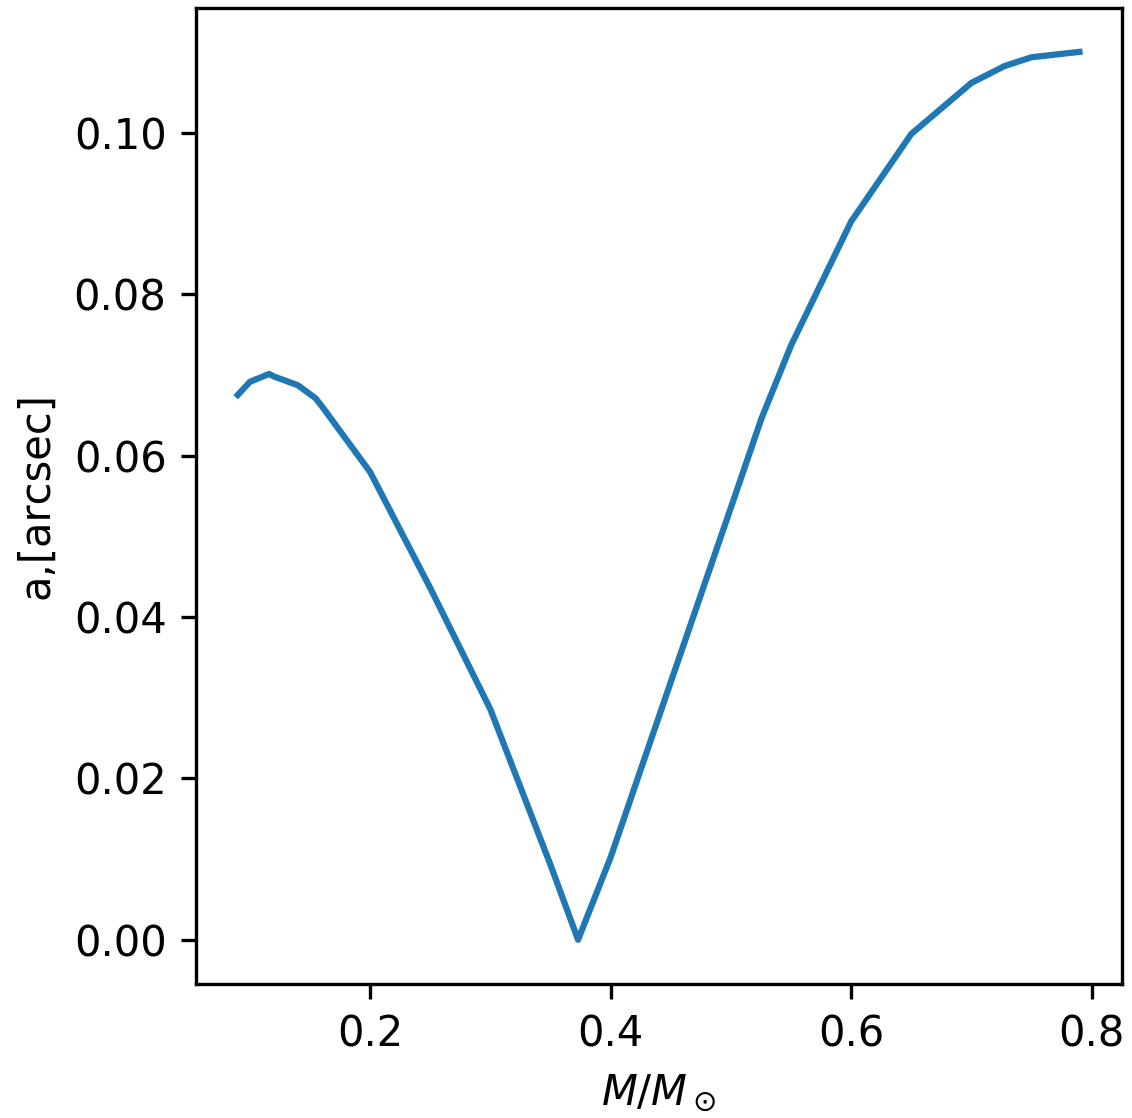
\includegraphics[width=0.6\textwidth]{semiaxis_vs_mass035_10_25.png}\\
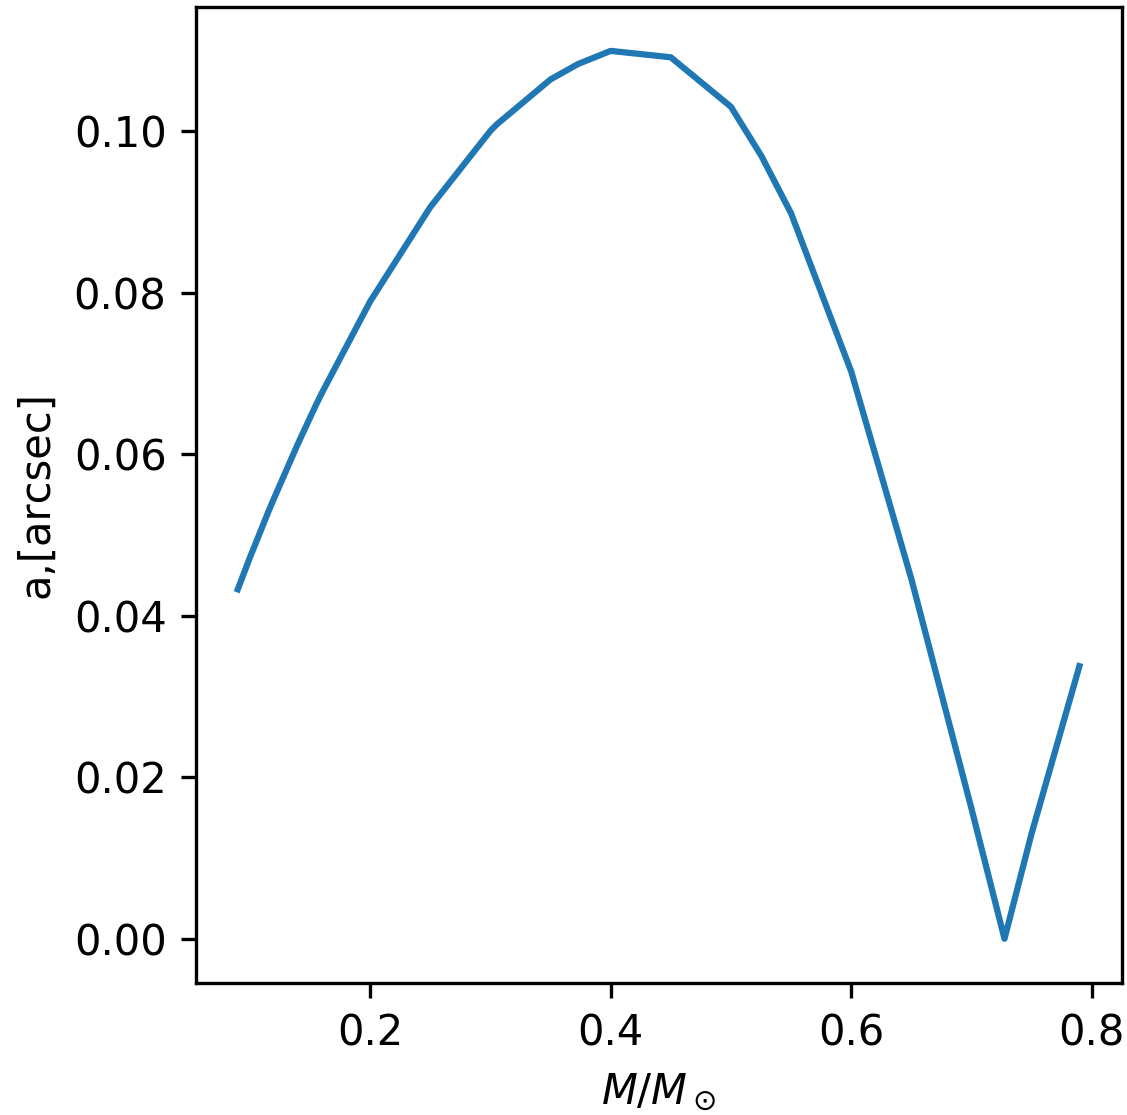
\includegraphics[width=0.6\textwidth]{semiaxis_vs_mass073_10_25.png}
\caption{Зависимость большой полуоси орбиты фотоцентра от отношения массы одной из компонент, если массу другой принять постоянной (для верхнего рисунка фиксирована масса $0.35\,M_\odot$, для нижнего "--- $0.73\,M_\odot$).}
\end{figure}

Представим себе двойную систему с большой полуосью в 10 а.е., удаленную от Солнца на 25~пк. Предположим, что плоскость орбиты совпадает с картинной плоскостью. Используя PARSEC-изохроны для солнечной металличности, несложно вычислить величину большой полуоси орбиты фотоцентра:
\begin{equation}
\label{eq:Photocenter}
 a_{ph}=a\left| \frac{M_2}{M_1+M_2} - \frac{L_2}{L_1+L_2} \right|,
\end{equation}
где $M_1,M_2,L_1,L_2$ соответственно массы и светимости компонент.

Далее, варьируя массы компонент несложно проследить, в как меняется $a_{ph}$. Рисунок~\ref{fig:semiaxis1} демонстрирует два примера поведения $a_{ph}$. Верхняя панель данного рисунка фиксирует $M_2 = 0.35\,M_\odot$, а $M_1$ меняется от $0.1\,M_\odot$ до $0.8\,M_\odot$, нижняя "--- соответствует неизменной массе $M_2 = 0.73\,M_\odot$.

Как следует из рисунка~\ref{fig:semiaxis1}, нелинейность зависимости <<масса -- светимость>> ведет к ненулевым значениям $a_{ph}$ на всем интервале, кроме случая равенства масс компонент. Для многих значений $M_1$ величина большой полуоси орбиты фотоцентра превышает 40~mas. Эта величина вполне может быть обнаружена с помощью наземных ПЗС-наблюдений. Например, если орбита круговая, а разность эпох составляет половину орбитального периода (для масс  $0.35\,M_\odot$ и $0.73\,M_\odot$ это около 30 лет), $\Delta\mu\approx 13~mas/yr$, что вполне <<детектируемо>> при точности собственных движений около $4~mas/yr$.  

Но этот вывод не дает полного представления об эффективности поиска  $\Delta\mu$-двойных. Важно оценить общее количество двойных систем, которое можно выявить таким способом. В следующем разделе мы представим соответствующий анализ.

\subsection{Оценка количества $\Delta\mu$-двойных среди близких карликов}\label{subsec:ch1/sect2/sub2}
Задача оценки количества двойных систем, состоящих из маломассивных звезд и проявляющих себя как $\Delta\mu$-двойные, относится к числу естественных вопросов, которые возникают при построении наблюдательной программы. Необходимо отметить, что максимально несмещенные оценки возможны только в том случае, когда известны  точно статистические параметры звездного населения солнечной окрестности: пространственная плотность распределения, функция  масс, доля двойных систем в зависимости от массы и металличности, соответствующие распределения для отношения масс компонент и орбитальных параметров. На сегодняшний день параметры этих функций и распределений известны ненадежно. И тем не менее можно попытаться провести оценку, привлекая данные из научной периодики. Для построения модельной популяции маломассивных двойных систем мы использовали функцию масс из работы \cite{2005ASSL..327...41C},
распределение больших полуосей из статьи \cite{2010ApJS..190....1R}. Мы исходили из подсчетов звезд в солнечной окрестности, произведенных коллаборацией RECONS \cite{2019AJ....157..216W} и данных Gaia DR2. В итоге в области, ограниченной радиусом 50 пк, с учетом доли двойных для маломассивных звезд оказалось чуть больше 14 тысяч двойных систем с $M<0.7\,M_\odot$. 

В дальнейшем были образованы звездные пары, расстояния до которых, галактические широты и долготы назначались случайным образом так, чтобы модельная популяция заполняла весь объем внутри сферы радиусом 50~пк. Для каждой двойной системы назначались орбитальные параметры согласно упомянутым литературным источникам. С учетом масс и светимостей компонент вычислялись большие полуоси орбит фотоцентров. Далее образовывались массивы координат, моделирующие ряды наблюдений для каждой звезды с учетом характерных значений случайных ошибок отдельных положений звезд. Эпохи модельных наблюдений соответствовали реальным. В итоге несложно было вычислить количество звезд, которые можно было бы детектировать как $\Delta\mu$-двойные.  На рисунке~\ref{fig:F-hist} показана часть распределения величин $F$, демонстрирующая относительную редкость $\Delta\mu$-двойных. Подсчет дает около 1000 таких систем на всем небе. Учитывая то, что в пулковскую программу были включены все звезды в зоне склонений	$30^\circ$ -- $70^\circ$, мы могли рассчитывать на детектирование примерно 250 звезд. 

\begin{figure}[pt]\label{fig:F-hist}
\centering
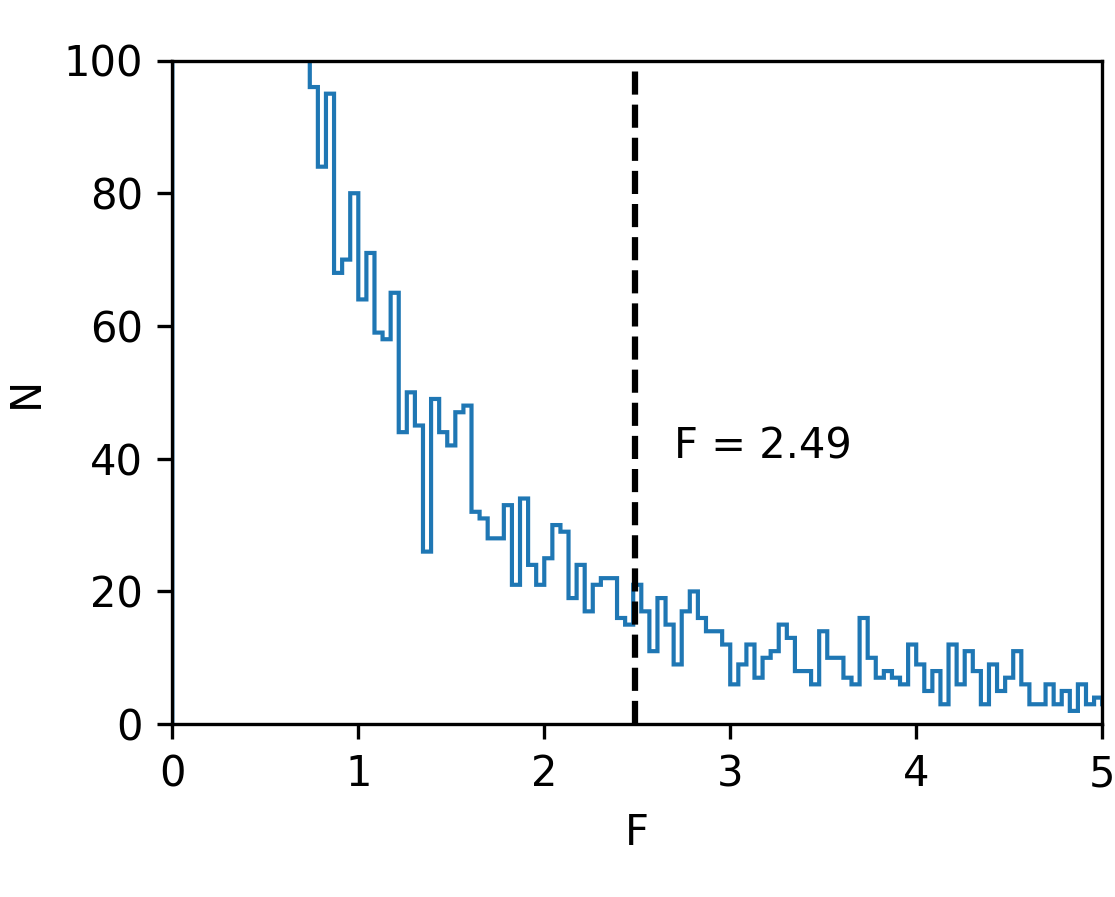
\includegraphics[width=0.9\textwidth]{F-hist.png}
\caption{Распределение величины $F$, полученное в ходе численного моделирования. Пороговое значение $F=2.49$ показано вертикальной линией. }
\end{figure}

Проведенные оценки показывают, что обнаружение $\Delta\mu$-двойных звезд вполне реально на основе доступных данных. Относительно невысокие точности наземных наблюдений сильно  ограничивают такой способ выявления двойных систем. Стоит ожидать серьезного прогресса в этой области исследований по мере публикации релизов миссии Gaia.

Полезным будет сопоставление реально наблюдаемых  $\Delta\mu$-двойных с модельными оценками, проведенными в этом разделе, так как это даст дополнительную информацию для анализа статистических свойств ансамбля двойных систем, образованных маломассивными карликами.

\subsection{Потенциальное количество звезд, двойственность которых проявляется в деформированности их изображений на ПЗС-кадрах}\label{subsec:ch1/sect2/sub3}

В данной работе мы полагаемся не только на анализ собственных движений, но и принимаем во внимание возможность анализа формы изображений.  Модельные эксперименты с изображениями звезд показали, что успех детектирования сильно зависит от отношения звездных величин компонент, углового разделения и характерного размера изображения одиночной звезды, который можно оценить с помощью FWHM звездных изображений. Очевидно, что фотоцентры компонент интересующих нас пар звезд должны лежать внутри области ПЗС-кадра, задаваемой FWHM. Причем уверенное детектирование возможно при угловом разделении $\rho>0.5FWHM$.  Данная величина в используемом материале меняется от $\approx\,1"$ до $\approx\,3"$.  В качестве оценки сверху для числа звезд, двойственность которых можно обнаружить таким способом, можно принять количество объектов из модельной популяции, описанной в разделе~\ref{subsec:ch1/sect2/sub2}, с разделениями в пределах от $0.5FWHM<\rho<FWHM$. На рис.~\ref{fig:rho-hist} показана гистограмма распределения двойных систем по величине углового разделения компонент $\rho$. Вертикальные линии определяют указанные выше значения FWHM, характерные для используемых ПЗС-кадров. В итоге суммирование дает оценку "--- около 3000 звезд по всему небу.  

\begin{figure}[pt]\label{fig:rho-hist}
\centering
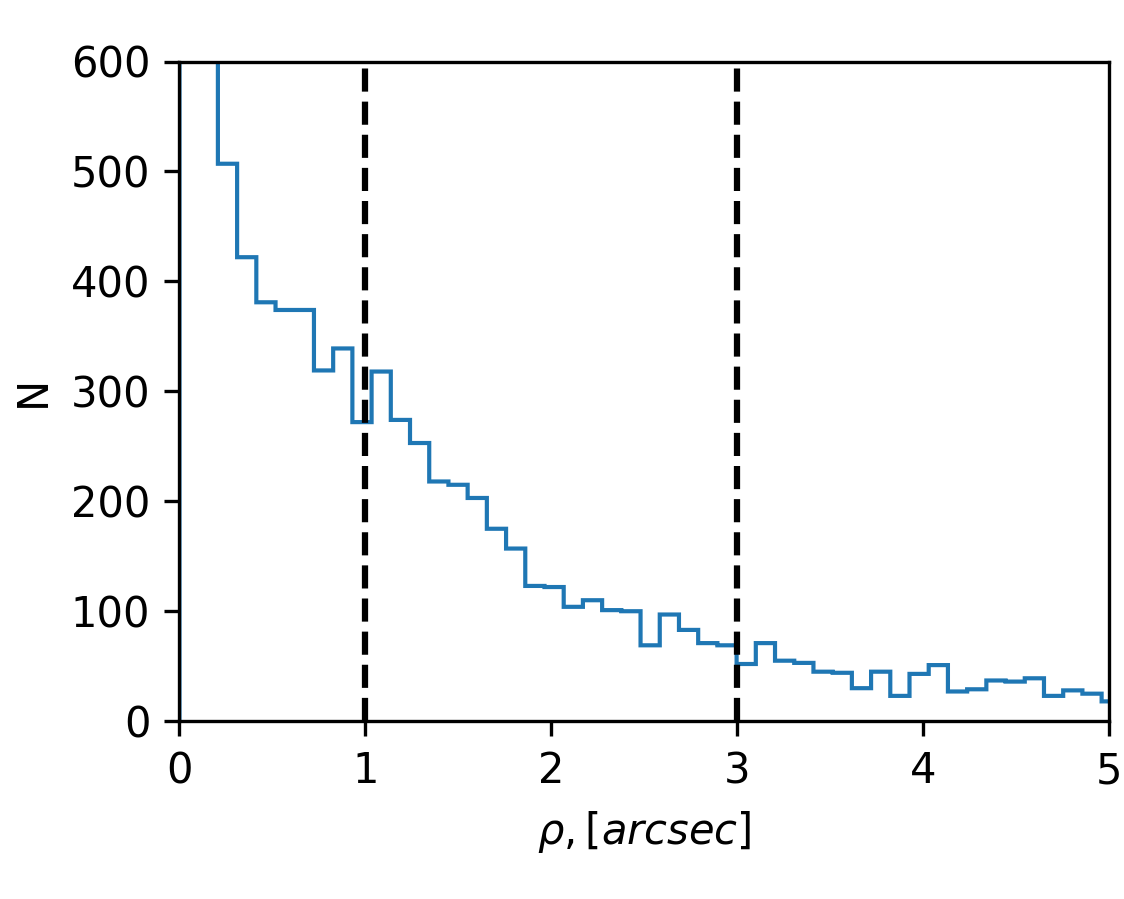
\includegraphics[width=0.9\textwidth]{rho-hist.png}
\caption{ Распределение угловых расстояний между компонентами для модельной популяции маломассивных двойных систем.}
\end{figure}

Однако следует помнить, что это всего лишь грубое приближение, которое должно совпасть с реальным значением по порядку величины. Полученный результат свидетельствует, что признаки двойственности могут быть обнаружены при анализе изображений примерно 20\,\% популяции двойных звезд.

\section{Анализ собственных движений, определенных на разных временных интервалах. Метод Вилена} \label{sec:ch1/sec3}
Как было показано в предыдущем разделе, выявление нелинейности движения по небесной сфере требует хорошей наблюдательной истории "--- нескольких десятков положений, полученных в разные эпохи. Свойства движений компонент двойных систем определили возможность массового поиска неразрешенных звездных пар без необходимости иметь большое количество точных положений. Достаточно иметь оценки собственных движений, полученные на разных временных интервалах. При высокой точности определения координат может хватать всего трех положений.

 Собственные движения определены для огромного количества звезд в ходе реализации разнообразных наблюдательных проектов. Это сделало возможным относительно массовое обнаружение звезд, которые имеют явные признаки двойственности. Высокая точность определения положений звезд с помощью  астрометрического спутника (порядка 1 mas) раскрыла новые пути поиска и исследования двойных систем \cite{1997ESASP1200.....E}. В 1999 году был представлен метод поиска неразрешаемых двойных систем, основанный на статистическом анализе наблюдаемых изменений собственных движений звезд \cite{1999A&A...346..675W}. В работе исследовались ярчайшие звезды, изученные в ходе миссии Hipparcos. Основная идея метода Вилена проиллюстрирована на рисунке~\ref{fig:widea}. Для физической одиночной звезды собственное движение, измеренное в течение короткого промежутка времени, в пределах точности измерений должно совпадать с собственными движением, полученным из очень длинного временного интервала. И в общем случае такого совпадения не будет наблюдаться для неразрешаемой двойной звезды. Из-за гравитационного влияния более слабой компоненты, движение фотоцентра двойной звезды будет волнообразным, что может определить значительное отличие мгновенно измеренного собственного движения от долгосрочного (в идеале "--- движение барицентра системы). Такую разницу в работе назвали <<космической ошибкой>> и обозначили как $\Delta\mu$. При значительном преобладании космической ошибки по сравнению с ошибкой измерения объект относился к кандидатам в двойные и обозначался как <<Дельта--мю двойная>> (<<$\Delta\mu$--binaries>>). Объекты, у которых космическая ошибка была в рамках ошибки наблюдений, были обозначены как <<кандидаты в одиночные звезды>>  (<<single--star candidate>>), если не было другой информации об их двойственной природе.

\begin{figure}[pt]
 \centering
 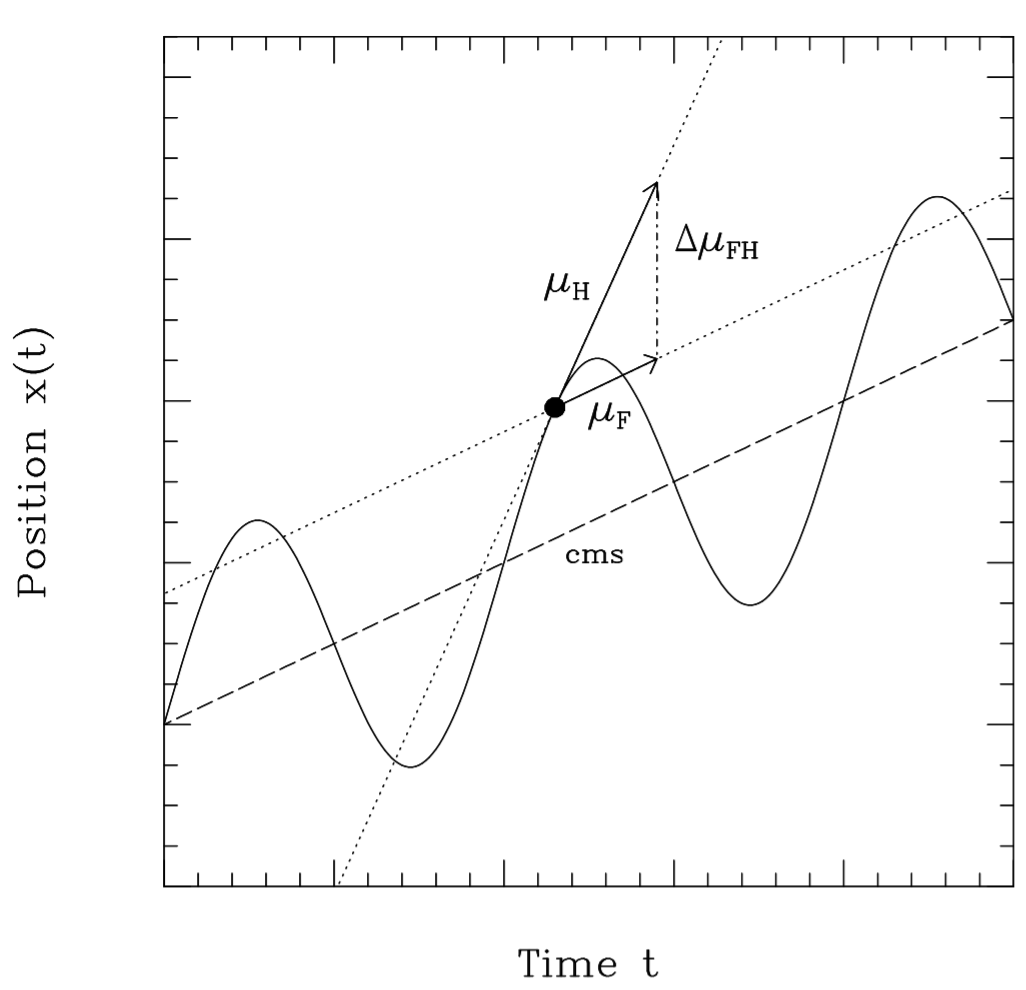
\includegraphics [scale=0.5] {Wielen-idea}
 \caption{Колебания фотоцентра двойной системы, вызванные влиянием орбитального движения, приводит к заметной разнице $\Delta\mu_{FH}$ между мгновенно измеренным собственным движением Hipparcos $\mu_{H}$ и средним собственным движением $\mu_{F}$ фотоцентра. Здесь период обращения двойной системы имеет среднюю длину ($\approx$\,30 лет), так что собственное движение $\mu_{F}$, полученное из наземных данных (например, из FK5), по существу равно собственному движению барицентра (cms) двойной звезды. Взято из \cite{1999A&A...346..675W}, Рис. 1.}
 \label{fig:widea}
\end{figure}

В качестве квази-мгновенных были взяты высокоточные собственные движения HIPPARCOS \cite{1997ESASP1200.....E}, $\mu_{H}$, полученные за период около 3 лет в 1991 году. В качестве квази-средних "--- собственные движения, полученные несколькими способами. 

В первую очередь для вычисления квазисредних (<<долгосрочных>>) собственных движений использовался каталог FK5 \cite{1988VeARI..32....1F}, \cite{1991VeARI..33....1F}. Из него были извлечены собственные движения ($\mu_F$), а также положения звезд для вычисления новых собственных движений совместно с положениями HIPPARCOS ($\mu_{0F}$), временная база которых составила в среднем 40 лет. Ошибки вычисленных собственных движений оказались значительно меньше, чем указанные в FK5. Их точность обеспечили относительно маленькие ошибки положений FK5 и значительная разница эпох FK5 и HIPPARCOS. Таким образом были получены по 3 разности собственных движений для каждой из координат $\delta$  и $\alpha ^*$~=~$\alpha\,\cos\delta$. Стоит отметить, что положения, взятые из FK5, для одной звезды могли не совпадать по эпохе для разных координат. Это несколько усложнило физическую интерпретацию результатов исследования, однако исключило корреляции в собственных движениях по разным координатам.

Помимо каталога FK5 в исследовании был использован каталог GC \cite{1936gcts.book.....B}. Хотя количество объектов GC (33\,342) сильно больше, чем в FK5 (4\,652), низкая точность собственных движений этого каталога не позволила использовать собственные движения, опубликованные в GC. Однако огромная разница эпох наблюдения с HIPPARCOS позволила получить новые собственные движения ($\mu_{0}$(GC)). Также стоит отметить, что большое пересечение выборки FK5 и GC обеспечило проверку согласованности данных.

Для вычисления ошибок получаемых $\Delta\mu$ авторы использовали ошибки собственных движений из каталога HIPPARCOS, а также комбинацию индивидуальных ошибок собственных движений наземных каталогов со значениями систематических ошибок редукции каталогов в систему HIPPARCOS.

В ходе исследования статистических особенностей данных авторы учли тот факт, что собственные движения HIPPARCOS по двум координатам коррелируют. По данным в каталоге коэффициентам корреляции была построена ковариация, которая позволила скорректировать (повернуть на угол $\psi$) оси собственных движений таким образом, чтобы они соответствовали осям эллипсоида ошибок (см. рисунок~\ref{fig:werr}). Вдоль новых осей авторами были определены формулы дисперсий ожидаемого гауссовского распределения ошибок.

Для оценки статистической значимости $\Delta\mu$ был выведен тестовый  параметр оценки $F_{0H}$:

\begin{equation}
  \label{eq:WiF}
  F^{2}_{0H} =\left(\frac{\Delta\mu_{0H,\psi}}{\epsilon_{\Delta\mu_{0H,\psi}}}\right)^{2}+\left(\frac{\Delta\mu_{0H,\bar{\psi}}}{\epsilon_{\Delta\mu_{0H,\bar{\psi}}}}\right)^{2}.
\end{equation}

Если звезда не является двойной, то ожидается, что некоррелированные переменные $\Delta\mu_{0H,\psi}$ и  $\Delta\mu_{0H,\bar{\psi}}$ будут следовать нормальным распределениям со средним нулем и дисперсиями, определенными авторами ранее. В этом случае вероятность $W(F)$ случайно найти значение $F_{0H}$, равное или превышающее наблюдаемое значение, определялось уравнением:

\begin{equation}
  \label{eq:WiW}
  W(F) = e^{-F^2_{0H}/2}
\end{equation}

Плотность вероятности $w(F)dF$, показывающая вероятность нахождения $F_{0H}$ между $F$ и $F+dF$ определяется как:

\begin{equation}
  \label{eq:Wiww}
  w(F) = -\frac{dW(F)}{dF} = F_{0H}\,e^{-F^2_{0H}/2}
\end{equation}

Характер поведения этих функций (см. рисунок~\ref{fig:wWw}) дал основание полагать, что высокое наблюдаемое значение $F_{0H}$ является значимым показателем двойственной природы исследуемого объекта. В качестве минимального значения $F_{0H}$, при котором звезду относили к $\Delta\mu$-двойным, авторы определили как $F_{lim,b}=3.44$, который дает $W(3.44)=0.0027$, что удовлетворяет критерию 3$\sigma$. Вторым пограничным значением $F_0H$, ниже которого звезда считалась кандидатом в одиночную стало $F_{lim,s}=2.49$, что соответствует критерию 2$\sigma$ ($W(2.49)=0.0456$).

 \begin{figure}[pt]
 \centering
 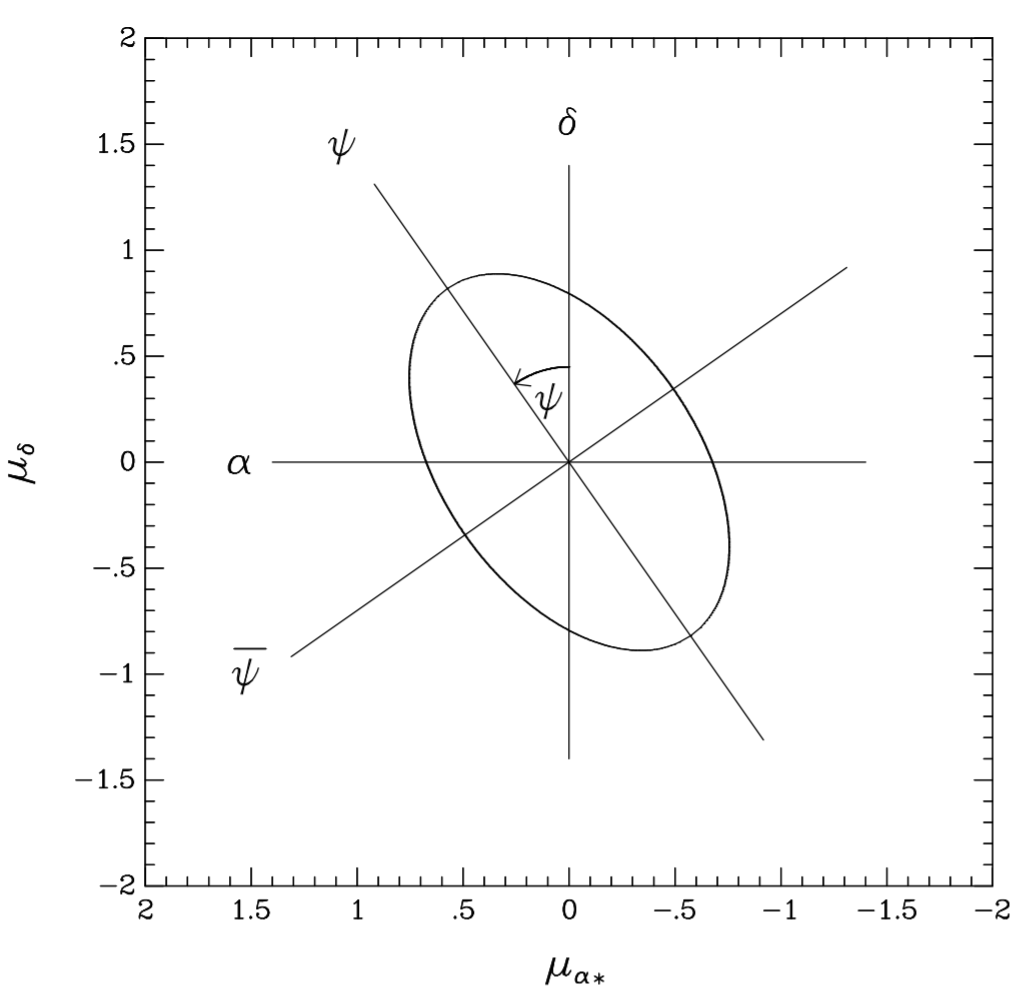
\includegraphics [scale=0.5] {Wielen-err}
 \caption{Эллипсоид ошибок измерений $\Delta\mu$, наклонен относительно экваториальной системы ($\delta$, $\alpha^*$) на угол $\psi$. Большая ось эллипсоида ошибок указывает в направлении $\psi$, малая ось "--- в направлении $\bar{\psi}$.  Взято из \cite{1999A&A...346..675W}, Рис. 2.}
 \label{fig:werr}
\end{figure}

Тогда как для звезд представленных только в CG есть только одно значение $F_{0}(GC)$, для звезд FK5 в общем случае доступно 3 параметра оценки ($F_{FH}$, $F_{0H}$, $F_{0F}$). Авторы предлагают считать объект $\Delta\mu$-двойным, если хотя бы 1 из величин больше, чем $F_{lim,b}$. Для кандидата в одиночную звезду, все значения должны быть меньше $F_{lim,s}$.

Авторы отмечают, что данный метод имеет ограничения. К примеру, он не применим к двойным звездам, чей период орбитального движения менее 3 лет, а для звезд с очень большими периодами (порядка 1000 лет) метод требует чрезвычайно высокой точности. Однако, он хорошо работает для близких быстрых звезд, чей период составляет десятки лет.  В результате проведенной работы было обнаружено больше тысячи впервые детектированных $\Delta\mu$-двойных звезд, что составило примерно 10\,\% от исследованных.

 \begin{figure}[pt]
 \centering
 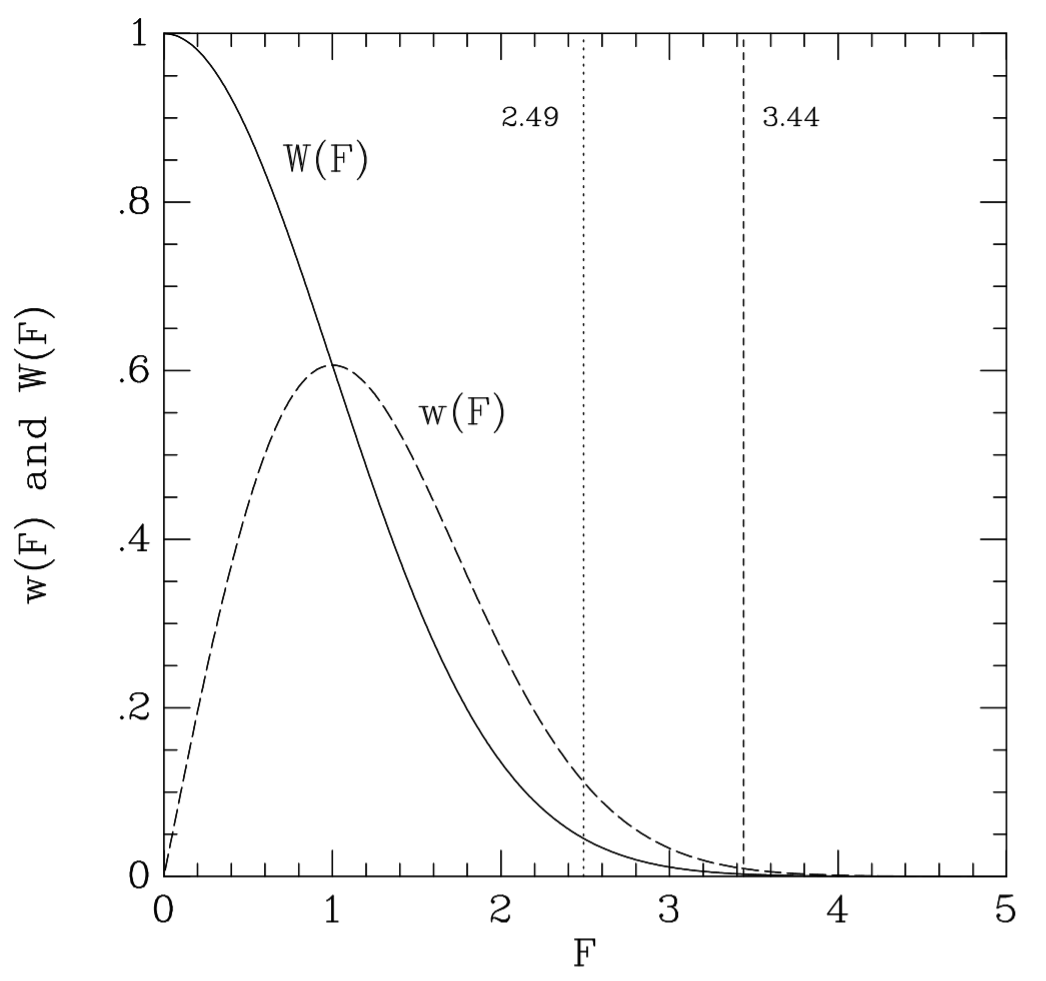
\includegraphics [scale=0.5] {Wielen-Ww}
 \caption{Функция W(F) описывает вероятность случайного нахождения наблюдаемого значения тестового параметра, большего чем F. Функция w(F) "--- плотность вероятности. Указаны два критических значения: F~>~3.44 для $\Delta\mu$-двойных и F~<~2.49 для кандидатов в одиночную звезду. Взято из \cite{1999A&A...346..675W}, Рис. 3.}
 \label{fig:wWw}
\end{figure}

Напомним, что исследования Вилена и его коллег затрагивают яркие звезды из состава FK5 и HIPPARCOS. В основном это объекты в диапазоне от солнцеподобных звезд до звезд ранних спектральных классов главной последовательности и гигантов, распределенные в ближайших 100 пк от Солнца. Объекты нашего исследования "--- звезды-карлики ближайшего окружения Солнца. Но, с некоторыми усовершенствованиями, идея Вилена вполне применима к поиску двойных систем для этого типа объектов. 

\section{Исследования близких карликов в Пулковской обсерватории} \label{sec:ch1/sec4}
В последнее десятилетие в Пулковской обсерватории активно реализуется комплексная программа изучения звезд с большими собственными движениями, включающая определение тригонометрических параллаксов  \cite{2010AstL...36..576K}, \cite{2013MNRAS.435.1083K}, уточнение собственных движений, анализ кинематики. В том числе реализуется изложенный выше подход к детектированию двойных карликов. Метод Вилена был адаптирован для исследования звезд низкой светимости с большими значениями собственного движения. Наиболее подробное изложение адаптации и реализации метода Вилена в пулковской программе будет представлено в главе~\ref{ch:ch3}. Первая попытка применения данного подхода \cite{2011AstL...37..420K} была предпринята на материале звезд-карликов, расположенных в зенитной зоне Пулковской обсерватории (от $30^\circ$ до $70^\circ$ по склонению). Наблюдения были проведены с помощью Нормального астрографа. В наблюдательную программу вошли 1123 звезды с большими собственными движениями ($\mu$~>~300~mas/yr). Следующая работа \cite{2015AstL...41..833K} содержит исследования практически всех быстрых звезд, относимых к категории близких карликов и доступных для наблюдений в Пулкове. Для дальнейшего анализа были вычислены собственные движения, однако в отличие от первой реализации положения звезд брались не из каталогов, а были получены методами прямой редукции с кадра на кадр, это позволило избежать систематических ошибок каталогов, однако встал вопрос о реализации способа вычисления пиксельных координат. На первом этапе использовался нелинейный МНК, однако в дальнейшем для определения параметров PSF хорошо зарекомендовал себя адаптированный для исследования изображений звезд метод shapelet-формализма, описанию которого посвящена следующая глава. Этот метод дал возможность осуществить выявление двойных звезд на основе особенностей их изображений, о чем подробнее сказано в главе ~\ref{ch:ch4}.           % Глава 1
\chapter{Применение shapelet-разложения для аппроксимации изображений звездообразных объектов} \label{ch:ch2}
Рассмотренная выше методика поиска $\Delta\mu$-двойных предполагает наличие положений и собственных движений, отнесенных к единой опорной системе. Это выполняется для ярких звезд (FK5, Hipparcos). Объекты нашего исследования преимущественно слабее $12^m$ и, обладая большими значениями собственных движений, нередко вообще не входят в астрометрические каталоги. Поэтому до недавнего времени репрезентация положений и собственных движений близких карликов в системе ICRF не была произведена. Некоторый прогресс в этом направлении появился после реализации проекта SUPERBLINK и появления каталога LSPM \cite{2005AJ....129.1483L}. Основой для LSPM стали сканы пластинок паломарского обзора. В результате были определены собственные движения для более 60 тысяч быстрых звезд в системе каталога Tycho--2.

Некоторая часть близких к Солнцу карликов представлена в таких каталогах как UCAC2, UCAC3, UCAC4, CMC14, 2MASS, SDSS. Поэтому на первом этапе реализации пулковской программы изучения звезд с большими собственными движениями была предпринята попытка учесть взаимные систематические ошибки между каталогами и привести положения интересующих нас объектов к единой системе \cite{2011AstL...37..420K}. Как оказалось, такой подход обладает рядом недостатков. Во-первых, для большинства интересующих нас звезд доступны всего два--три положения. Во-вторых, часто систематические ошибки возникают на уровне обработки ПЗС-кадров, поэтому их учет по данным только астрометрических каталогов крайне затруднен. В связи с этим возникла необходимость провести новые наблюдения в течение нескольких лет. Что и было произведено с помощью пулковского Нормального астрографа. Для многих обзоров оказались доступны цифровые архивы. Например, оцифрованные паломарские пластинки, кадры из проектов 2MASS, SDSS, WISE несложно массово загрузить с помощью простых скриптов. В дальнейшем оказалось возможным провести астрометрическую редукцию цифровых кадров и, тем самым, гарантировать привязку собственных движений к единой системе хотя бы для необходимых участков неба.

Все это потребовало аппроксимации звездных изображений и определения пиксельных положений их фотоцентров. Традиционно для такого рода вычислений выбирают модель PSF, которая зависит от свойств изображений конкретного обзора. Создание столь разветвленного алгоритма, учитывающего специфику разного материала, является весьма громоздкой задачей. Логично было искать единый метод аппроксимации, который легко адаптируется под любые ПЗС-кадры или сканы фотопластинок.

Для числовой интерпретации характеристик наблюдаемых сигналов сейчас  доступны многочисленные сложные пакеты анализа данных (например,  FOCAS in IRAF, \cite{1981AJ.....86..476J}; SExtractor, \cite{1996A&AS..117..393B}), а также существуют различные методики: например, вейвлет-анализ, введенный А.Гроссманом и Ж.Морле в 1982 году в работе, посвященной проблеме анализа сейсмических сигналов, и впоследствии нашедший широкое применение в различных науках, в том числе и в астрономии, а также Метод оптимального вычитания изображения \cite{1998ApJ...503..325A}  или, например, Метод наблюдения слабого линзирования \cite{1995ApJ...449..460K}, разработанный для исследования эффекта гравитационного микролинзирования галактик через анализ их изображений. Перед нами стояла задача найти и адаптировать для наших целей метод, который смог бы в режиме массовой обработки наблюдений  анализировать изображения отдельных звезд, предоставляя информацию об особенностях характеристик этих изображений и с хорошей точностью вычисляя фотоцентры в пиксельных координатах.

Для решения большого класса астрономических задач модель изображения астрономических объектов на ПЗС-кадрах представляют в виде функции $I(x,y)$, определяемыми параметрами которой являются координаты фотоцентра изображения $x_{ph},y_{ph}$, уровень фона $I_{bgr}$, константы, описывающие размер и форму изображения ($a,b,c$). В самом простом случае это может быть двумерная гауссова функция:
 \begin{equation}
 \label{eq:ShI}
 I(x,y) = I_{bgr}+I_{max}\cdot e^{-(a\cdot(x-x_{ph})^2+b\cdot(y-y_{ph})^2+c\cdot(x-x_{ph})\cdot(y-y_{ph}))}.
 \end{equation}
 
На практике такая модель часто оказывается неполной. Для решения этой проблемы нередко прибегают к представлению изображения в виде взвешенной суммы функций, принадлежащих какой-нибудь ортогональной системе. Интересным примером в данном контексте является шейплет-формализм. Весьма подробно этот метод анализа изображений рассмотрен в серии статей Рефрегиера и его соавторов \cite{2003MNRAS.338...35R}, \cite{2003MNRAS.338...48R} и \cite{2005MNRAS.363..197M}. Поскольку алгоритм поиска двойных звезд в данной работе основан на этом методе, ниже приводится краткое описание формализма.

В декартовых координатах система базисных функций может быть представлена так:\\
\begin{equation}
\label{eq:ShBasis}
\phi_n(x) = \left(2^n\sqrt{\pi}n!\right)^{-\frac{1}{2}}H_n(x)e^{-\frac{x^2}{2}}.
\end{equation}
\\Здесь $H_n(x)$ "--- полином Эрмита порядка $n$ ($n$ "--- целое неотрицательное число), $\xi$ "--- независимая вещественная переменная.
Первые несколько одномерных базисных функций показаны на рис. 19. Эти функции (<<шейплеты>>) можно рассматривать как возмущения формы вокруг гауссианы $\phi_0(x)$.

\begin{figure}[h]
\centering
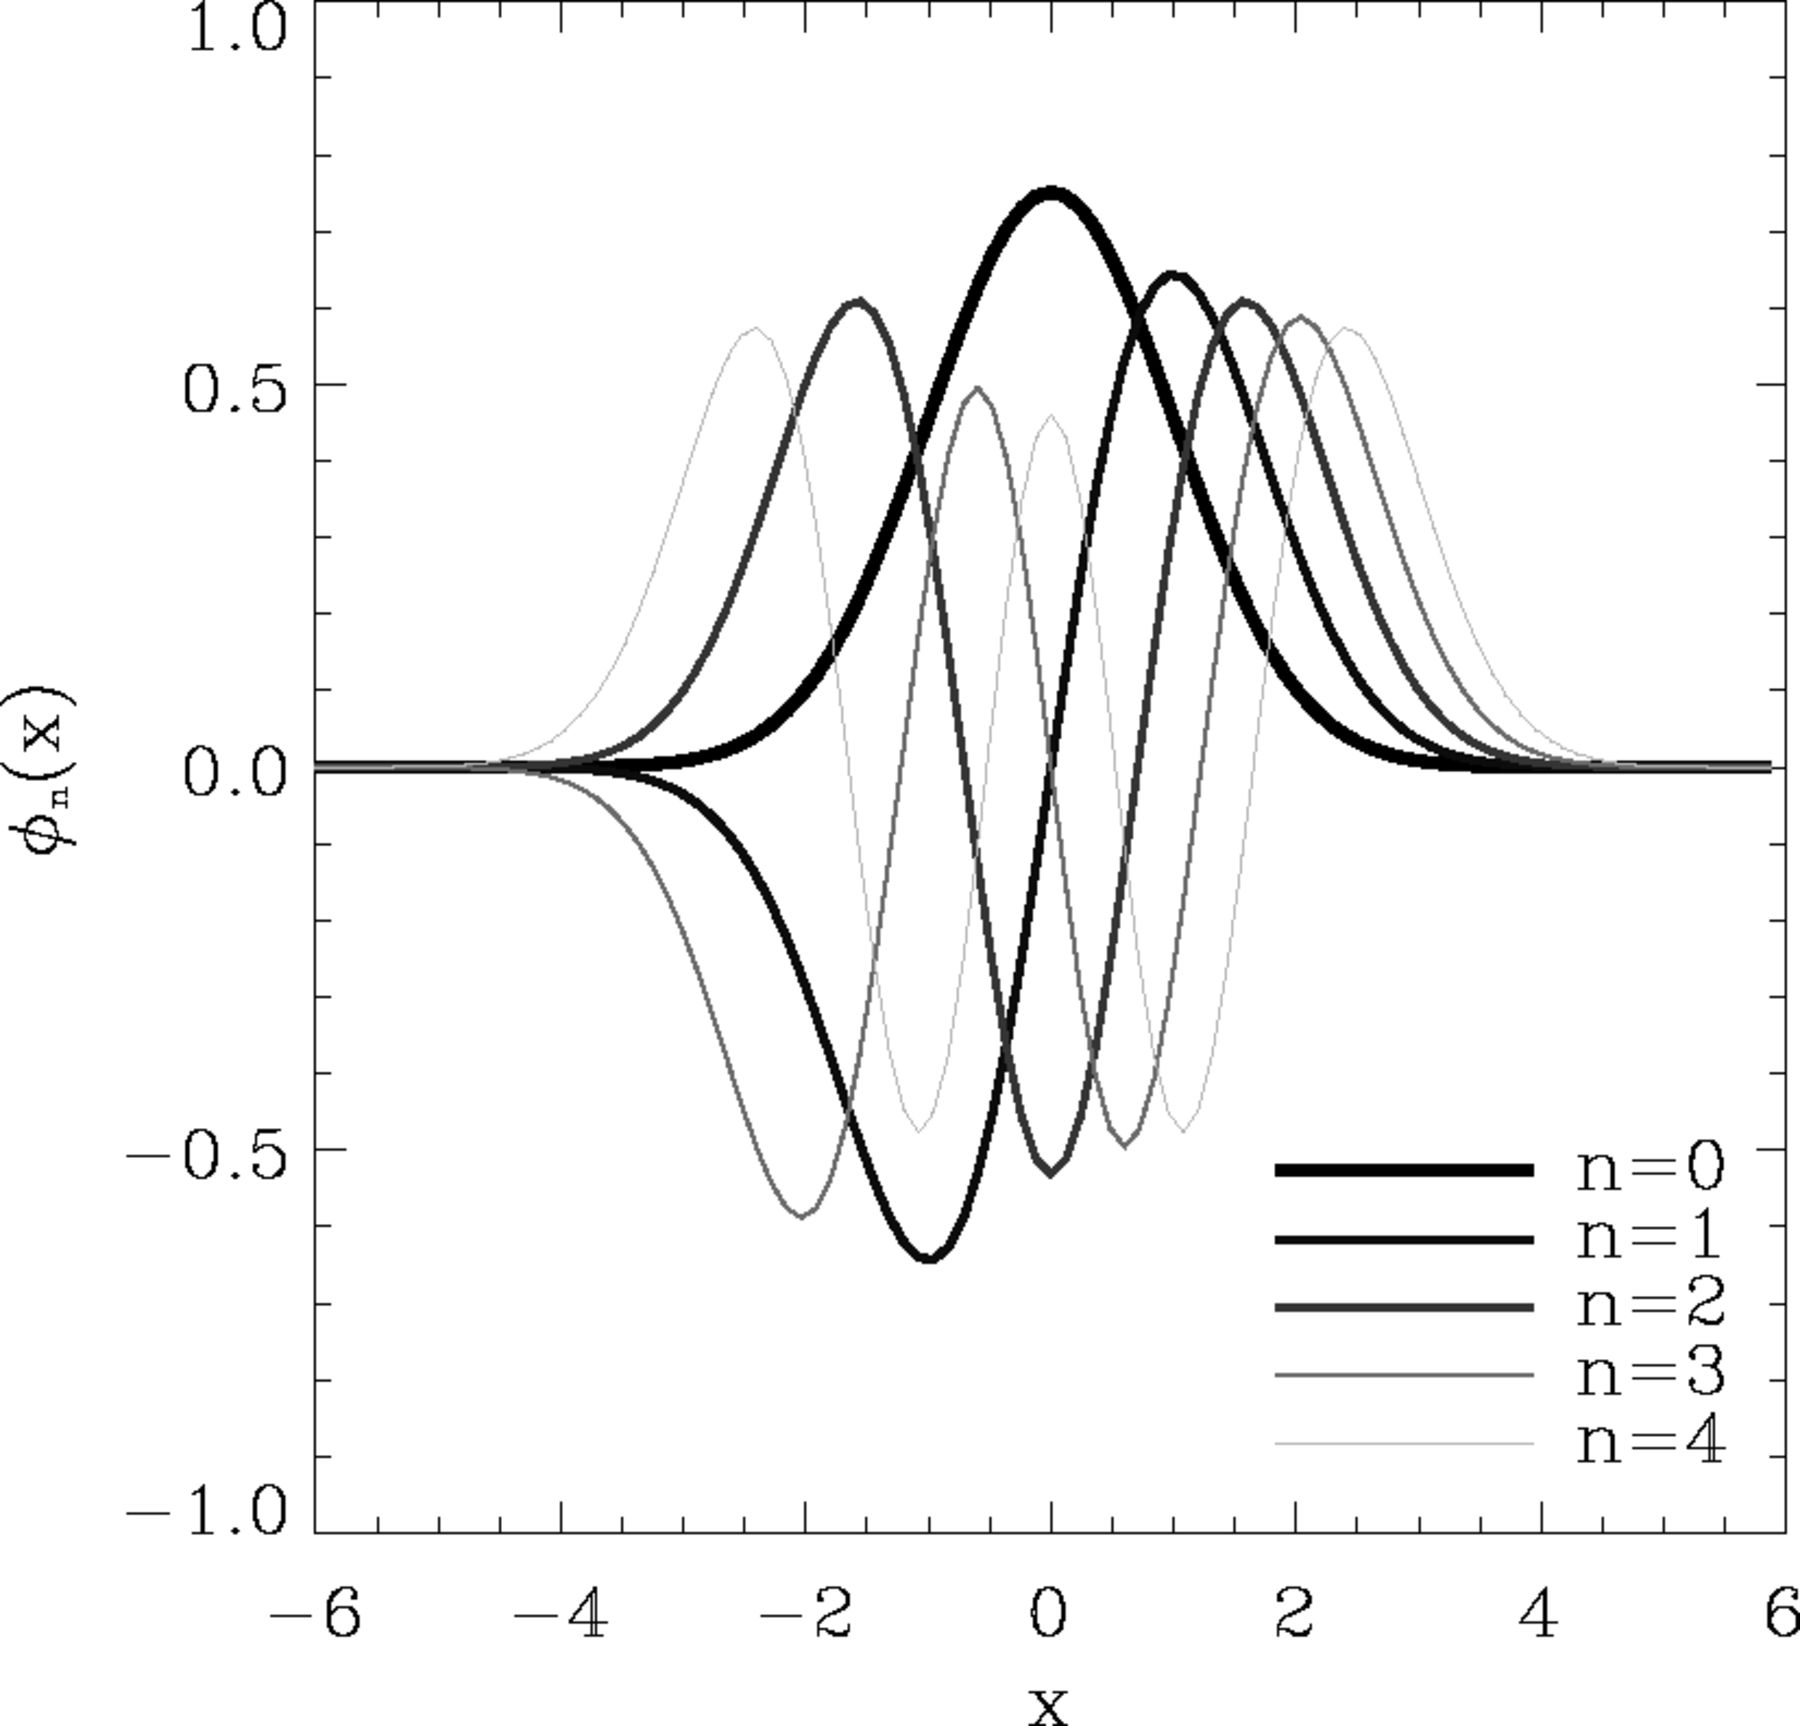
\includegraphics [scale=0.85] {refregier-1}
\caption{Первые несколько одномерных базисных функций $\phi_n(x)$. Взято из \cite{2003MNRAS.338...35R}, рис. 1.}
\label{fig:Sh1}
\end{figure}

Для двумерного случая удобно пользоваться представлением:\\
\begin{equation}
\label{eq:shape-basis-functions}
B_{n_1,n_2}(\beta,x,y,x_{ph},y_{ph}) = \beta^{-1}\cdot\phi_{n_1}\left(\frac{x-x_{ph}}{\beta}\right)\cdot\phi_{n_2}\left(\frac{y-y_{ph}}{\beta}\right).
\end{equation}
\\Здесь параметр $\beta$ "--- характерный размер изображения. В первом приближении его часто приравнивают стандарту двумерной гауссианы при $a=b$. В этом случае хорошей оценкой является $\beta = FWHM/2.35$ ($FWHM$ "--- ширина профиля звездного изображения на половине максимального отсчета). Индексы $n_1,n_2$ в формуле~\ref{eq:shape-basis-functions}  "--- порядки полиномов Эрмита по осям $x$ и $y$.

Таким образом изображение может быть представлено в виде:\\
\begin{equation}
\label{eq:image-shapelet}
I(x,y) = I_{bgr}+\sum_{n_1,n_2=0}^{\infty}f_{n_1,n_2}\cdot B_{n_1,n_2}(\beta,x,y,x_{ph},y_{ph}),
\end{equation}
\\где $f_{n_1,n_2}$ коэффициенты шейплет-разложения соответствующих порядков $n_1,n_2$.
Изображения первых нескольких двумерных функций представлены на рис. 20. Опять же, их можно рассматривать как возмущения вокруг двумерной гауссианы $\phi_{00}$.

\begin{figure}[h]
\centering
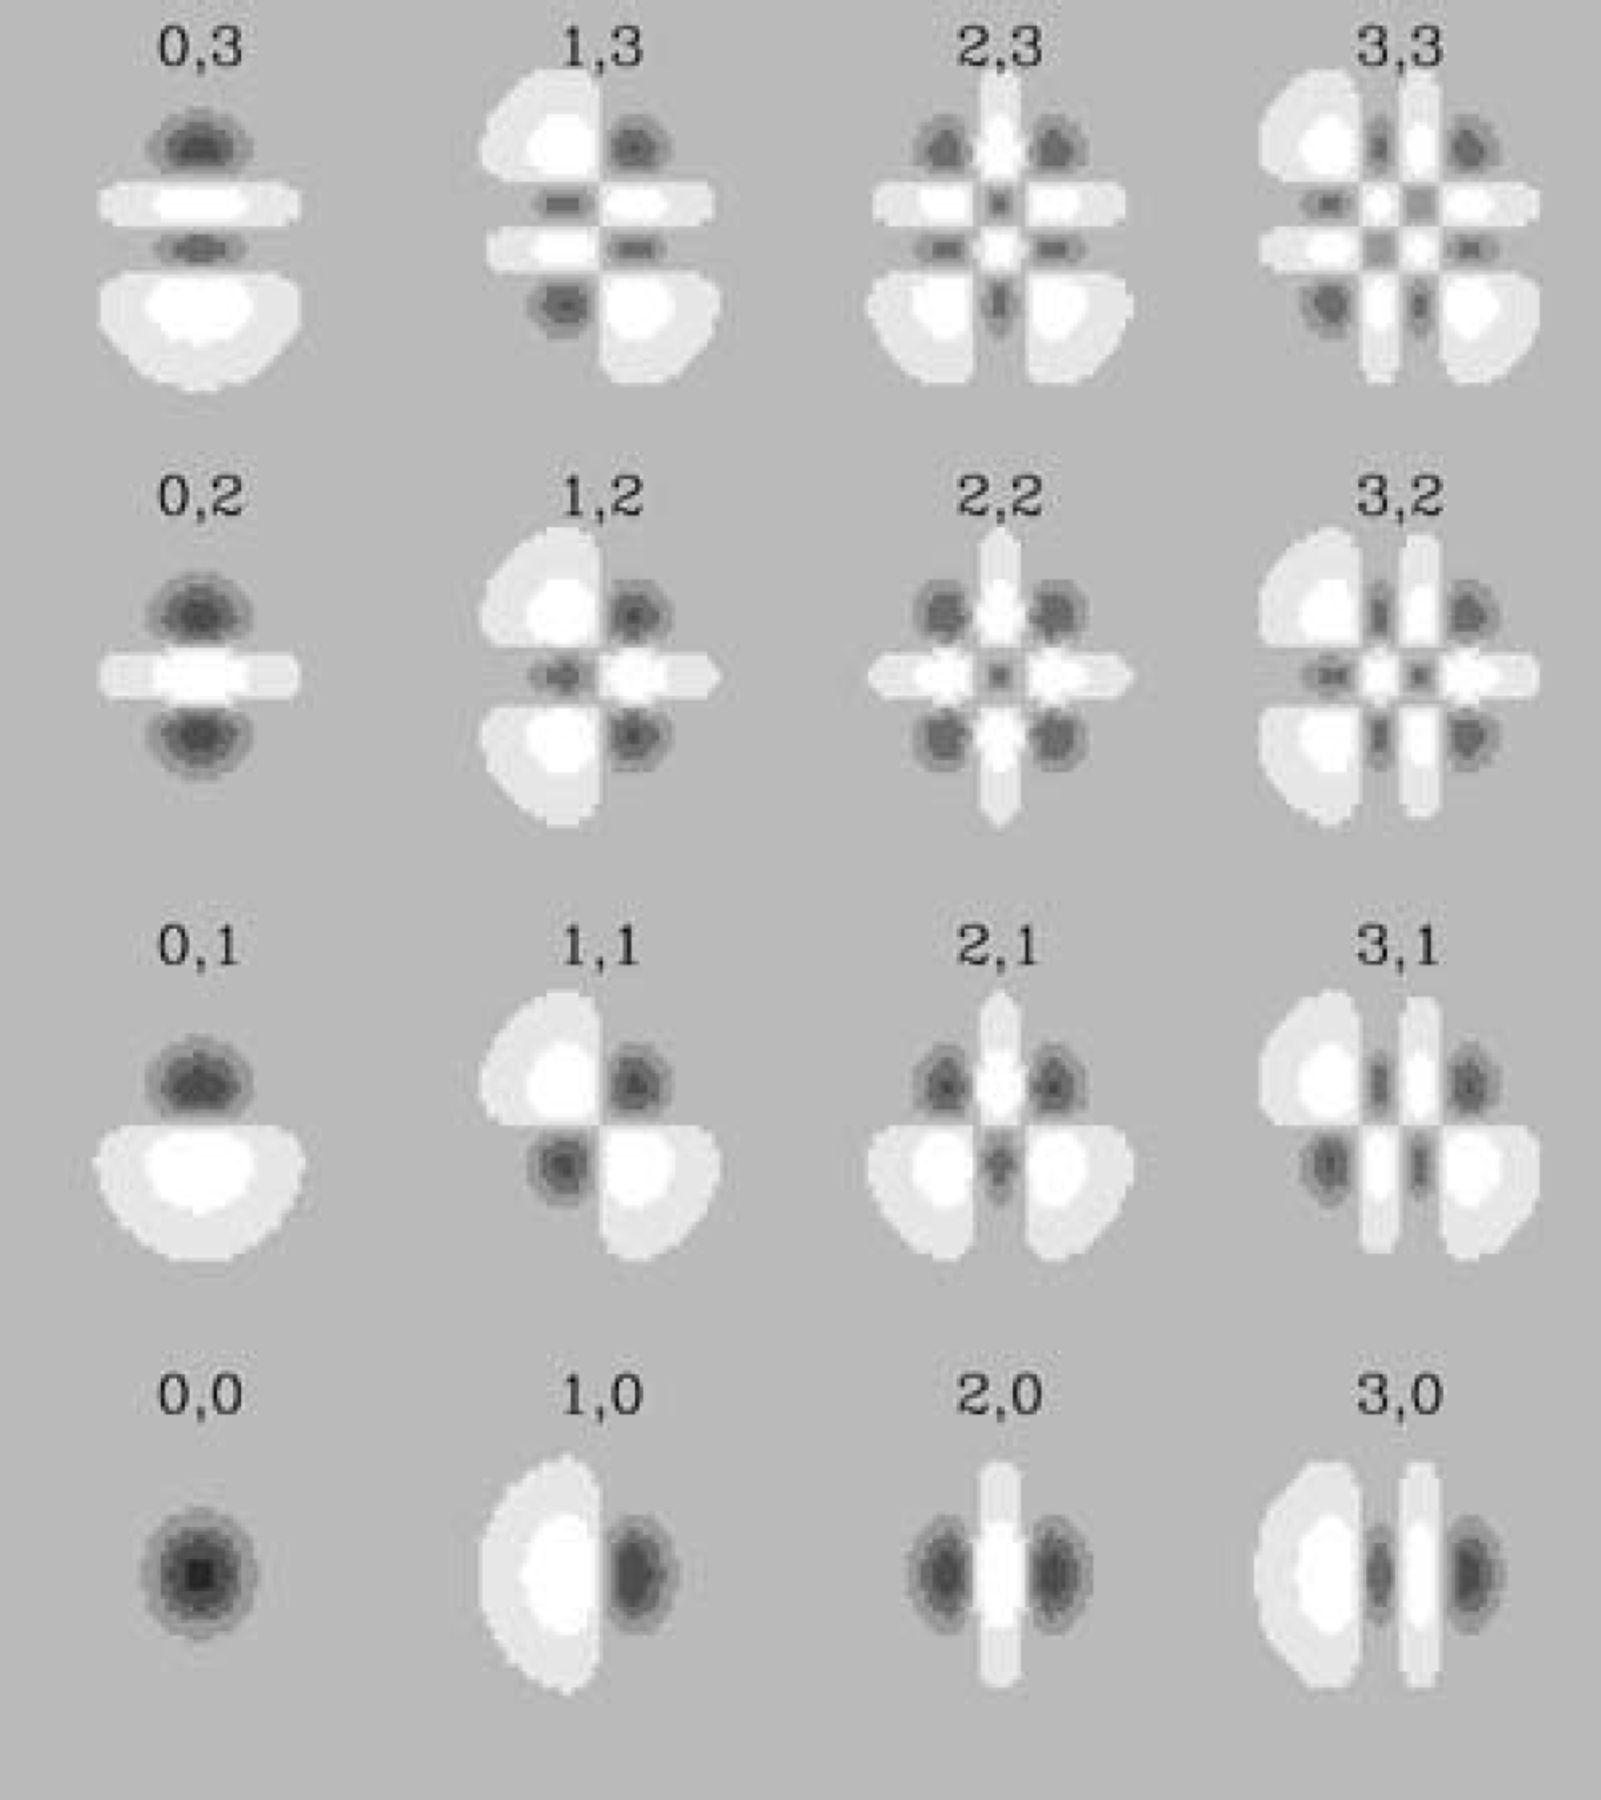
\includegraphics [scale=0.85] {refregier-2}
\caption{Первые несколько двумерных декартовых базисных функций. Темные и светлые области иллюстрируют положительные и отрицательные значения соответственно. Взято из \cite{2003MNRAS.338...35R}, рис. 2}
\label{fig:Sh2}
\end{figure}

Несмотря на то, что $B_{n_1,n_2}(\beta,x,y,x_{ph},y_{ph})$ "--- система ортогональных функций, на практике для оценки $f_{n_1,n_2}$ удобнее пользоваться методом наименьших квадратов. Это связано с тем, что суммирование производится в небольшой области ПЗС-кадра (например, 40$\times$40 пикселей). Ряд обрывают при условии $n_1+n_2=n_{max}$, так как при больших $n_1,n_2$ ошибка единицы веса становится меньше стандарта шума изображения. Это значит, что в систему шейплет-коэффициентов проникает информация, характеризующая случайные колебания отсчетов от пикселя к пикселю, а не свойства изображения астрономического объекта. Поэтому приближенное равенство стандарта шума и ошибки единицы веса рассматривается как условие для подбора оптимального значения $n_{max}$.  Примеры аппроксимации изображений одиночной и двойной звезды показаны на рис.~\ref{fig:model-stars} и рис.~\ref{fig:model-bin-stars}. Видно, что при $n_{max}=9$ в результате вычитания модельного изображения из исходного не остается заметной систематической составляющей.

\begin{figure}
\centering
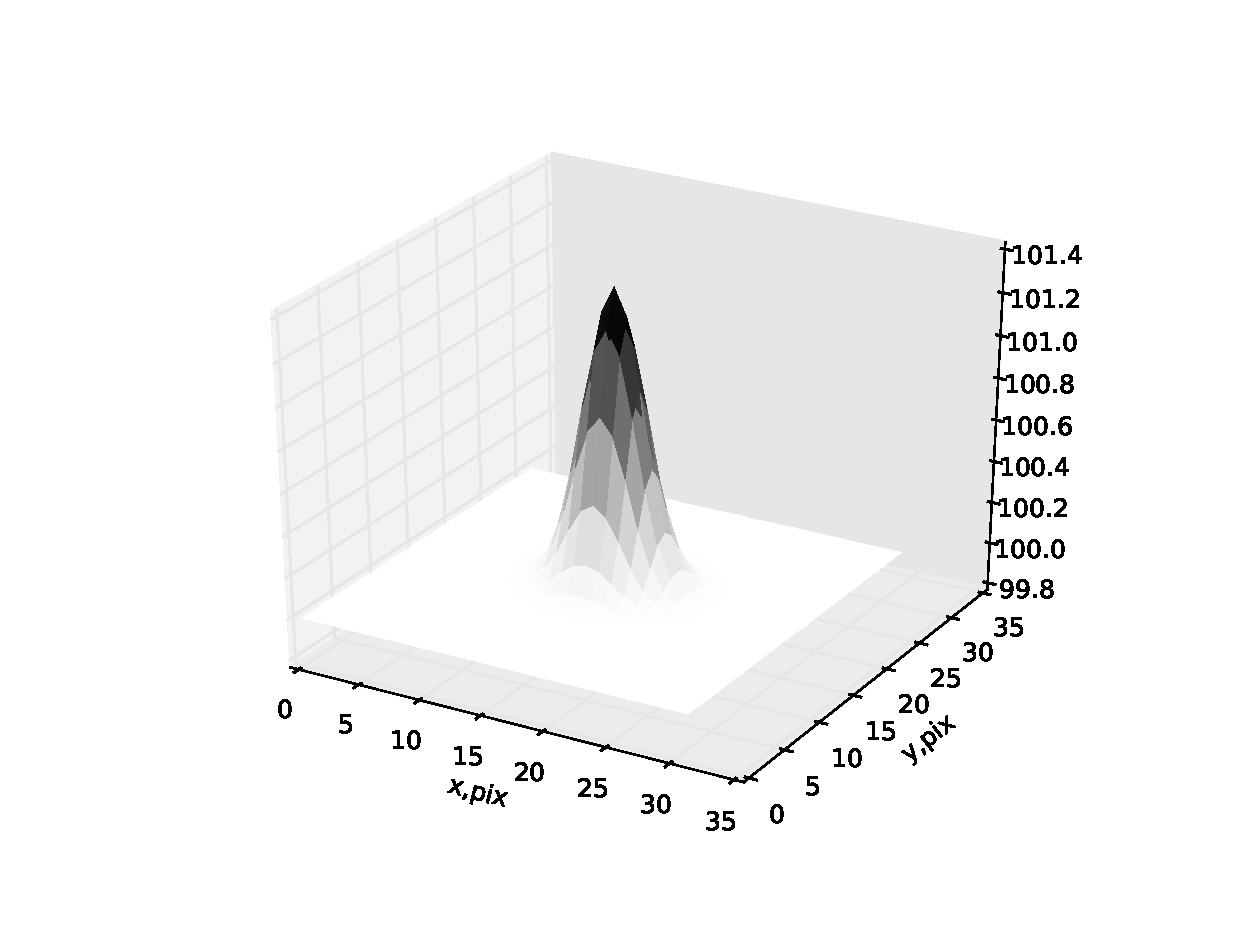
\includegraphics[width=0.49\columnwidth]{stimg_0.eps}
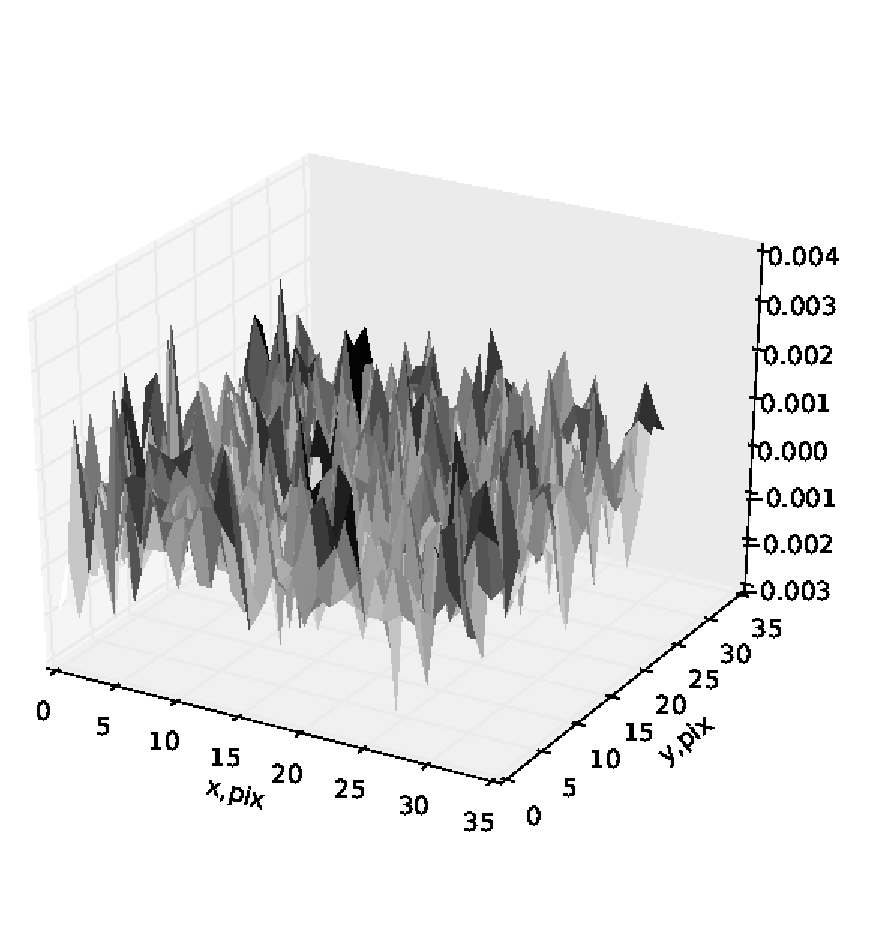
\includegraphics[width=0.49\columnwidth]{res_0.eps}
%\setcaptionmargin{5mm}
%\captionstyle{normal}
\caption{Изображение одиночной звезды (слева) и результат вычитания из реального изображения его модели (справа), построенной посредством shapelet-разложения.}
\label{fig:model-stars}
\end{figure}

\begin{figure}
\centering
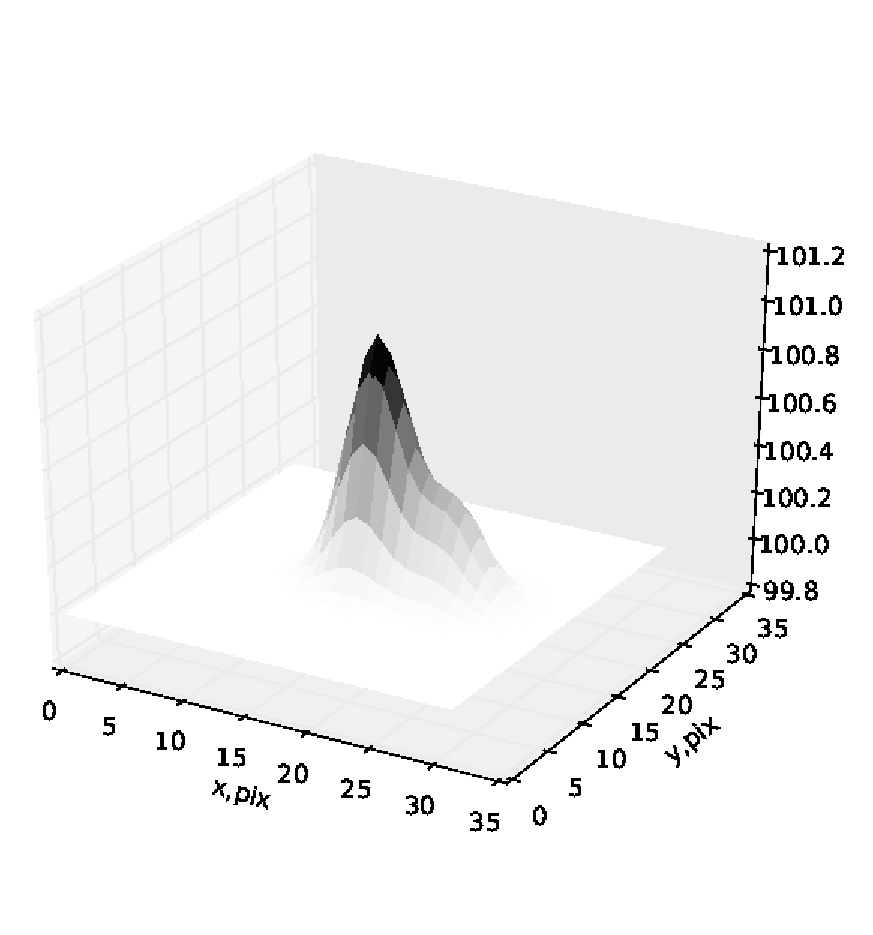
\includegraphics[width=0.49\columnwidth]{stimg_6.eps}
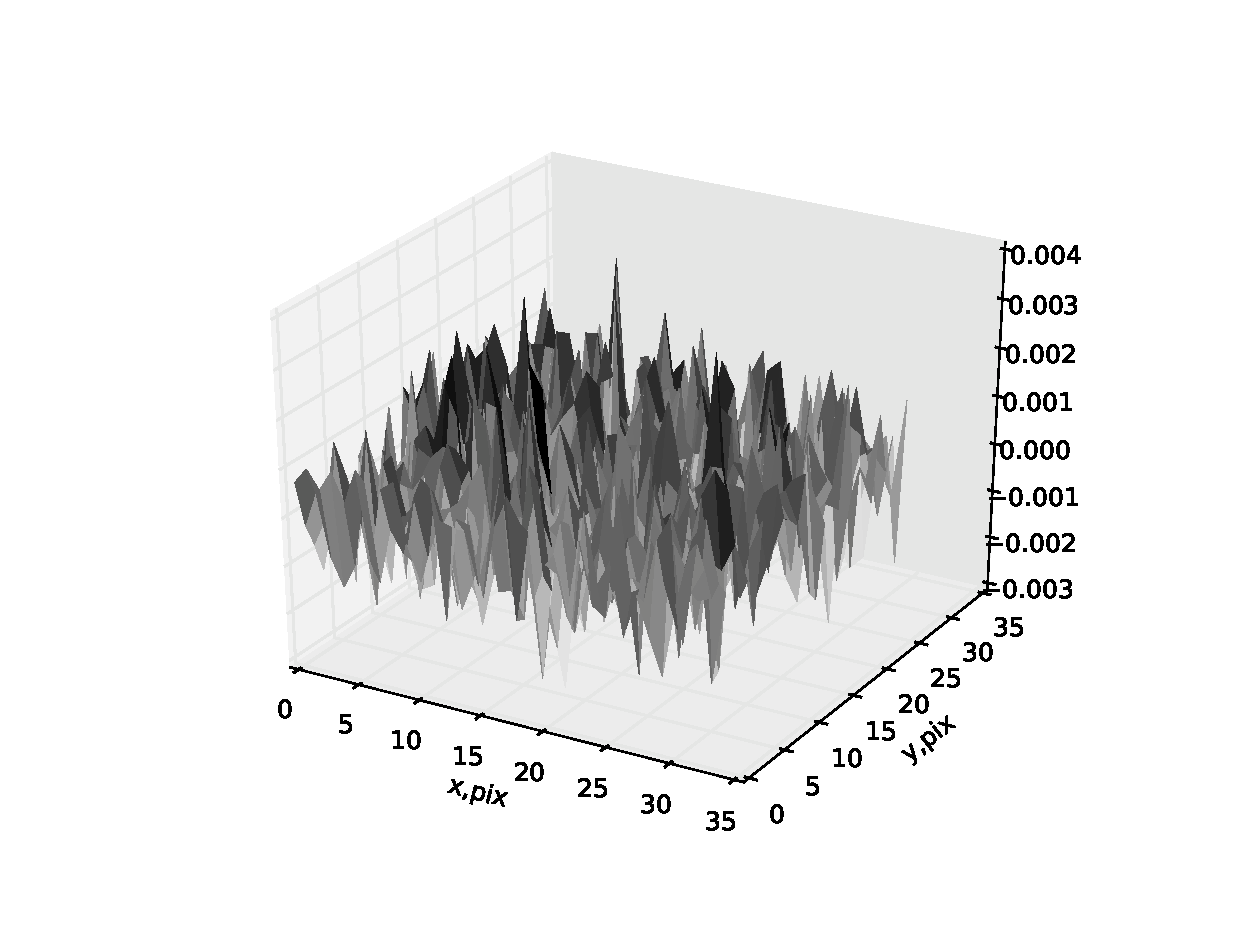
\includegraphics[width=0.49\columnwidth]{res_6.eps}
%\setcaptionmargin{5mm}
%\captionstyle{normal}
\caption{Слева дано изображение двойной звезды ($\Delta m=1^m$, $\rho=6$ pix). Справа "--- результат вычитания из реального изображения его модели.}
\label{fig:model-bin-stars}
\end{figure}

Привлекательность шейплет-формализма состоит не в только в относительной простоте реализации, но и в том, что многие свойства изображения естественным образом вычисляются на основе коэффициентов разложения $f_{n_1,n_2}$. Так, формула для расчета суммарного потока ($F$) принимает вид:
\begin{equation}
\label{eq:SHFlux}
 F = \sqrt{\pi} \beta \sum^{even}_{n_1,n_2} \sqrt{2^{2-n_1-n_2}C^{\frac{n_1}{2}}_{n_1}C^{\frac{n_2}{2}}_{n_2}}f_{n_1,n_2}
\end{equation}
Здесь \textit{<<even>>} означает, что суммирование выполняется только для четных индексов $n_1,n_2$. $C^{p}_{q}$ "--- биномиальные коэффициенты для соответствующих индексов.

Положение центра светимости можно выразить формулой:
\begin{equation}
\label{eq:SHPhCent}
x_1^f = \sqrt{\pi} \beta^2 F^{-1} \sum^{odd}_{n_1}\sum^{even}_{n_2} \sqrt{
(n_1+1)2^{2-n_1-n_2}C^{\frac{n_1+1}{2}}_{n_1+1}C^{\frac{n_2}{2}}_{n_2}}f_{n_1,n_2}.
\end{equation}
Здесь \textit{<<odd>>} означает суммирование по нечетным индексам $n_1,n_2$, \textit{<<even>>} "--- по четным. $C^{p}_{q}$ "--- биномиальные коэффициенты для соответствующих индексов (для $x_2^f$ "--- аналогичное выражение).

Также стоит упомянуть, что через shapelet-разложение можно успешно анализировать форму изображения звезд. Это реализуется через квадрупольные моменты изображения,  вычисляемые по формулам:

\begin{align}\label{moments}
 q_{xx} & = F^{-1} \sqrt{\pi} \beta^3 \sum^{even}_{n_1,n_2} (1+2n_1) \sqrt{2^{2-n_1-n_2}C^{\frac{n_1}{2}}_{n_1}C^{\frac{n_2}{2}}_{n_2}}f_{n_1,n_2} \\
 q_{yy} & = F^{-1} \sqrt{\pi} \beta^3 \sum^{even}_{n_1,n_2} (1+2n_2) \sqrt{2^{2-n_1-n_2}C^{\frac{n_1}{2}}_{n_1}C^{\frac{n_2}{2}}_{n_2}}f_{n_1,n_2} \\
 q_{xy} & = F^{-1} \sqrt{\pi} \beta^3 \sum^{odd}_{n_1,n_2} \sqrt{(n_1+1)(n_2+1)2^{2-n_1-n_2}C^{\frac{n_1+1}{2}}_{n_1+1}C^{\frac{n_2+1}{2}}_{n_2+1}}f_{n_1,n_2}
\end{align}

Здесь \textit{<<odd>>} означает суммирование по нечетным индексам.
Более подробно о применении квадрупольных моментов для анализа формы изображений описаны в главе~\ref{ch:ch4}.

Итак, как мы видим, shapelet-формализм позволяет эффективно решать задачу аппроксимации изображений звезд на сканах астронегативов и ПЗС-кадрах. Для реализации этого подхода в рамках данного исследования разработан соответствующий код на С++ и Python.
           % Глава 2
\chapter{Исследования собственных движений быстрых звезд в Пулковcкой обсерватории. Адаптация метода Вилена} \label{ch:ch3}
\section{Наблюдения быстрых звезд в Пулковской обсерватории. Вычисление новых собственных движений с использованием положений звезд из различных различных каталогов} \label{sec:ch3/sect1}
В ЛАЗА ГАО РАН  реализуется программа астрометрических исследований близких карликов \todo{(Хруцкая и др., 2009)}, в том числе и с привлечением оригинальных пулковских наблюдений. Основная часть наблюдений выполнена с помощью Нормального астрографа ($D=330$~мм, $F=3467$~мм).  Кроме того, используются наблюдения  26$''$--рефрактора ($D=650$~мм, $F=10\,413$~мм), благодаря относительно большому фокусному расстоянию которого удалось выполнить наблюдения с целью определения тригонометрических параллаксов звезд \todo{(Хруцкая и др., 2010, Ховричев и др., 2013)}. Часть наблюдений проводится на метровом зеркальном телескопе Сатурн \todo{(Ховричев и др., 2015b)}, который после восстановления активно используется для наблюдений тел Солнечной системы и быстрых карликов.

В 2011 году была опубликована работа \todo{(Хруцкая и др., 2011)}, посвященная исследованию собственных движений быстрых звезд низкой светимости. Это можно назвать первым этапом апробации метода Вилена с применением пулковских наблюдений. Для данного исследования были взяты наблюдения быстрых ($\mu>300 mas/yr$ по данным каталога LSPM \todo{(Лепин, Шара, 2005; Лепин и др. 2008)}) звезд, проводимых с 2006 года на Нормальном астрографе Пулковской обсерватории в зоне склонения $+30^{\circ}$~--~$+70^{\circ}$. В результате обработки около 10\,000 кадров 1123 включенных в программу наблюдения звезд были получены положения 414 объектов. Для аппроксимации звездных изображений использовался профиль Лоренца, параметры функции рассеивания точки (PSF) рассчитывались в кольце радиусом 20~пикселей. Астрометрическая редукция проводилась в два этапа, при этом использовался метод шести постоянных в системе  HCRF/UCAC3. UCAC3 \todo{(Захарис и др., 2010)} в качестве опорного был выбран в связи с него высокой плотностью распределения звезд по небесной сфере. Однако стоит отметить, что при работе с данным каталогом пришлось проявить некоторую осторожность из-за больших систематических ошибок собственных движений звезд северного полушария, что было отмечено авторами  каталога PPMXL \todo{(Розер и др., 2010)}. В ходе первого этапа редукции были вычислены ошибки на основе остаточных разностей пиксельных координат и проведен анализ на уравнение блеска, что было учтено на втором этапе редукции. В итоге ошибки единицы веса по обеим координатам в среднем составили 70~mas. Однако, стандартные ошибки средних положений звезд по нескольким кадрам оказались в основном в рамках 10~--~20~mas. Распределение стандартных ошибок определения экваториальных координат представлено на рисунке~\ref{fig:11erpos}

\begin{figure}[h]
 \centering
 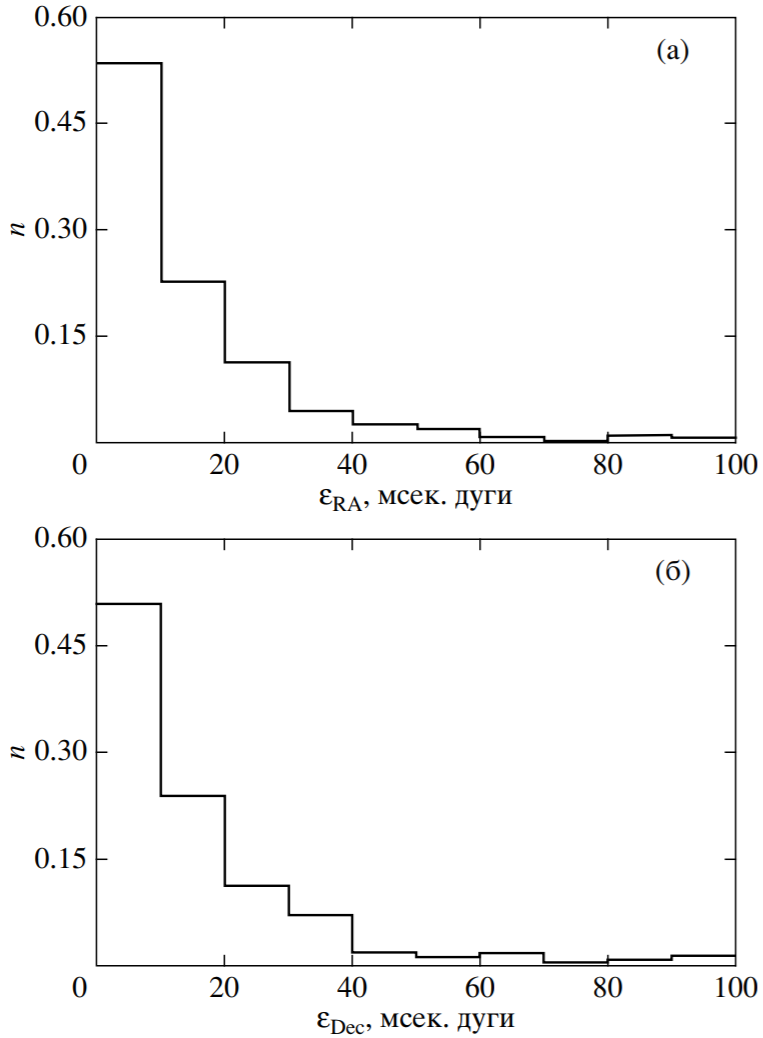
\includegraphics [scale=0.5] {khrutskaya3}
 \caption{Распределение стандартных ошибок определения экваториальных координат быстрых звезд, полученных в рамках работы \todo{Хруцкая и др., 2011}. Взято из указанной работы, рис. 3.}
 \label{fig:11erpos}
\end{figure}

Для расчета собственных движений помимо оригинальных положений были использованы координаты звезд из различных обзоров, в том числе CMC14, M2000, 2MASS, а также актуальный на тот момент SDSS DR7. Средние эпохи наблюдений этих каталогов лежат в пределах 1997~--~2004~г., стандартные ошибки в среднем составляют 40~--~80~mas. Координаты звезд в использованных каталогах формально отнесены к системам HCRF/UCAC2 или HCRF/Tycho--2, которые на приемлемом уровне точности можно соотносить с системой HCRF/UCAC3. Разности эпох для расчета собственных движений составили 6~--~13~лет, а средняя точность получившихся собственных движений оказалась в пределах 1~--~10~mas/yr (см. рисунок~\ref{fig:11ermu}).

\begin{figure}[h]
 \centering
 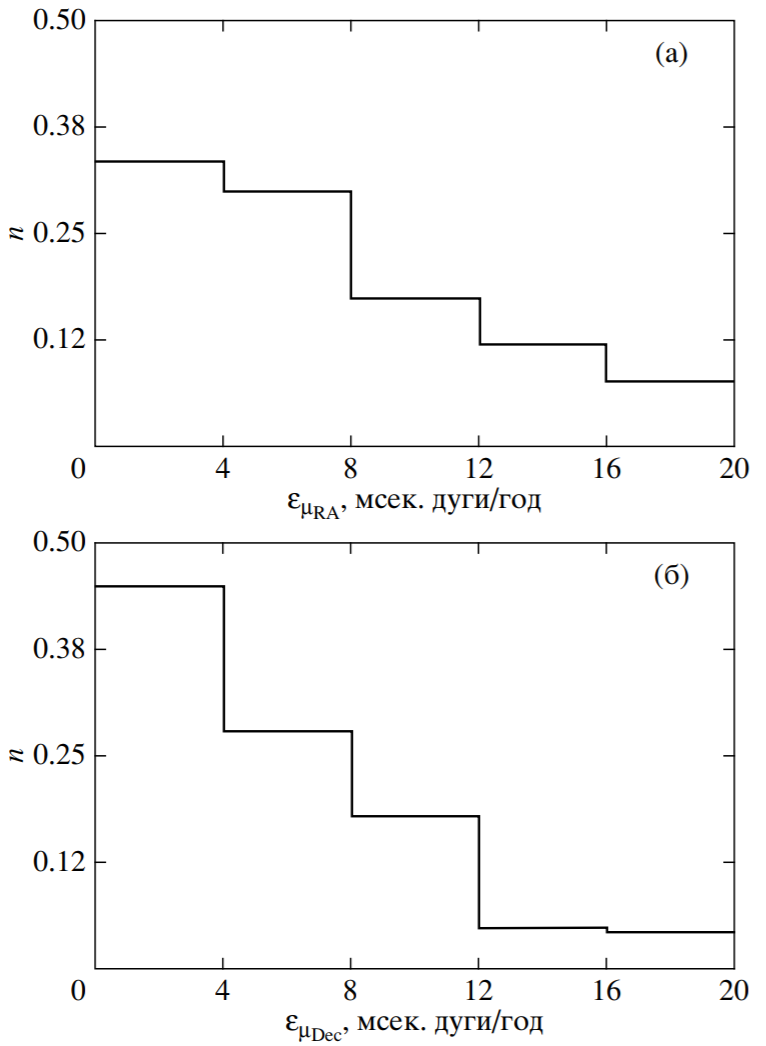
\includegraphics [scale=0.5] {khrutskaya4}
 \caption{Распределение стандартных ошибок определения собственных движений быстрых звезд, полученных в рамках работы  \todo{Хруцкая и др., 2011}. Взято из указанной работы, рис. 4.}
 \label{fig:11ermu}
\end{figure}

Далее для исследуемых звезд по аналогии с методом, описанном в главе 1., сравнивалась значимость по отношению к ошибкам определения разности полученных собственных движений и движений каталога LSPM, рассчитанной на временной базе около 50 лет. В данном случае полученные собственные движения можно считать квазимгновенными, а взятые из каталога LSPM "--- квазисредними. Значимость таких разностей (\glqq космических ошибок\grqq\  в терминологии Р. Вилена) была оценена через параметр F:
\begin{equation}
\label{eq:KhrF}
F^2=\frac{\Delta\mu^2_{RA}}{\epsilon^2_{\mu_{RA}}}+
\frac{\Delta\mu^2_{Dec}}{\epsilon^2_{\mu_{Dec}}}
\end{equation}
где $\Delta\mu_{RA}$ и $\Delta\mu_{Dec}$ "--- разности компонент квазисредних и квазимгновенных собственных движений звезды, а $\epsilon_{\mu_{RA}}$ и $\epsilon_{\mu_{Dec}}$ "--- соответствующие среднеквадратические ошибки. Кандидатом в $\Delta\mu$--двойную с вероятностью 95\% считалась звезда при $F>2.59$. Таких звезд оказалось 70 из выборки. В качестве проверки в работе было отмечено, что среди исследованных оказалось 42 звезды из каталога WDS \todo{(Мэсон и др., 2001)}, у 15 из которых были обнаружены значительные величины параметра F.
\section{Вычисление собственных движений на основе прямой редукции пиксельных координат} \label{sec:ch3/sect2}
Необходимо обратить внимание, что в работе, описанной в предыдущем разделе, имеют место некоторые недостатки. Во-первых, стоит отметить, что положения звезд в использованных каталогах лишь формально относятся к единой системе, неизвестные взаимные систематические ошибки могли оказать серьезное влияние на конечный результат. Кроме того, использовать F--статистику напрямую из работы Вилена было отчасти неправомерно. Ведь в оригинальной работе Вилена рассматривались ярчайшие звезды каталога HIPPARCOS и их высокоточные собственные движения, полученные в течение периода около 3 лет. Это гарантировало \glqq гауссовость\grqq\  распределения ошибок.

В качестве логичного продолжения предыдущей работы, было принято решение провести исследования собственных движений быстрых звезд, рассчитанных методом прямой редукции пиксельных координат с кадра на кадр, а также более тщательно оценить предельные величины параметра F, учитывая исследуемый материал.
\subsection{Формирование списка звезд и особенности наблюдений} \label{subsec:ch3/sect2/sub1}
Как и в предыдущей работе \todo{(Хруцкая и др., 2011)}, в программу наблюдений были включены звезды каталога LSPM. В основной список вошли 1972 звезды до $17^m$ в зоне склонений от $30^{\circ}$ до $70^{\circ}$. В основном это звезды c $\mu>300$~mas/год (1507 звезд). По разным причинам были добавлены 465 звезд. Некоторые из них имеют большое значение фотометрического параллакса, ряд звезд был добавлен для анализа возможности исследований сравнительно медленно двигающихся объектов ($\mu>100$~mas/год).

Распределение звезд наблюдательной программы по небесной сфере показано на рисунке~\ref{fig:15alloc}. Рисунок~\ref{fig:15hist} демонстрирует как программные объекты распределены по величине полного собственного движения, по блеску, по массам и расстояниям от Солнца. В целом, это почти полная выборка. Каталог LSPM содержит почти все существующие быстрые звезды до $19^m$ (Лепин и Шара, 2005 ). Поэтому можно сказать, что в пулковскую наблюдательную программу вошли все звезды, которые только можно эффективно наблюдать в Пулкове в соответствующих диапазонах по блеску и величине собственного движения.

\begin{figure}[h]
\centering
%\includegraphics [scale=1] {fig_1.ps}
\includegraphics[width=0.4\columnwidth]{fig1_a.eps}
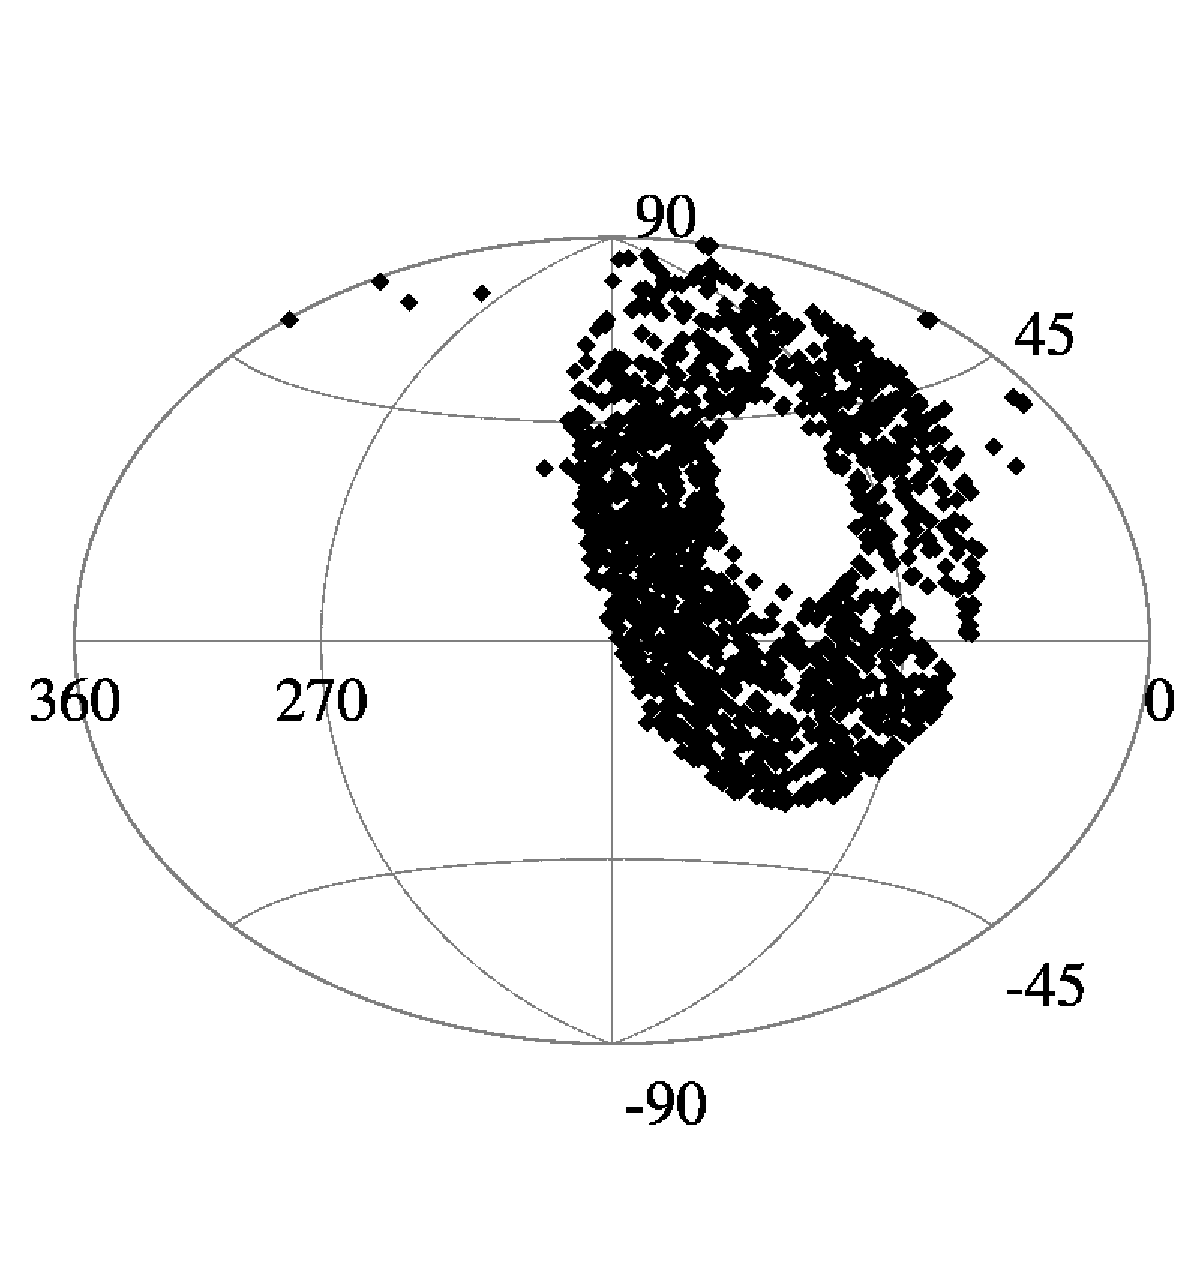
\includegraphics[width=0.4\columnwidth]{fig1_b.eps}
\caption{Распределение звезд пулковской программы по небесной сфере в экваториальной (слева) и галактической (справа) системах координат.}
 \label{fig:15alloc}
\end{figure}

\begin{figure}[h]
\centering
% \includegraphics [scale=1] {fig2.ps}
\includegraphics[width=0.4\columnwidth]{fig2a.eps}
\includegraphics[width=0.4\columnwidth]{fig2b.eps}
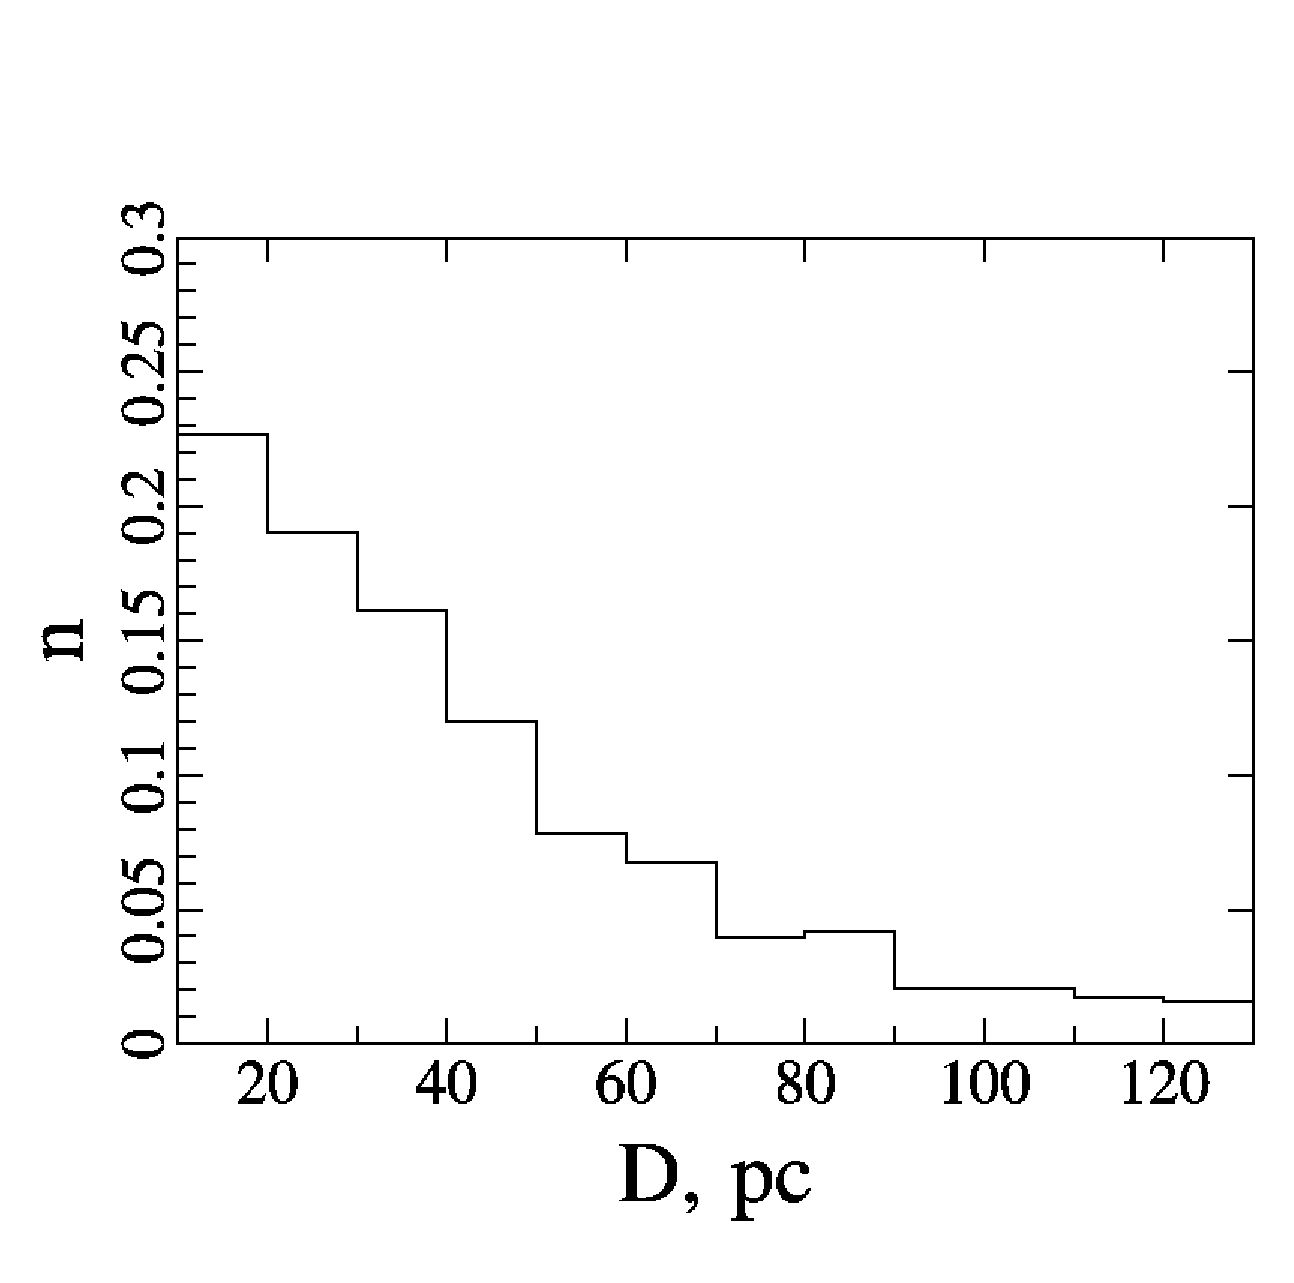
\includegraphics[width=0.4\columnwidth]{fig2c.eps}
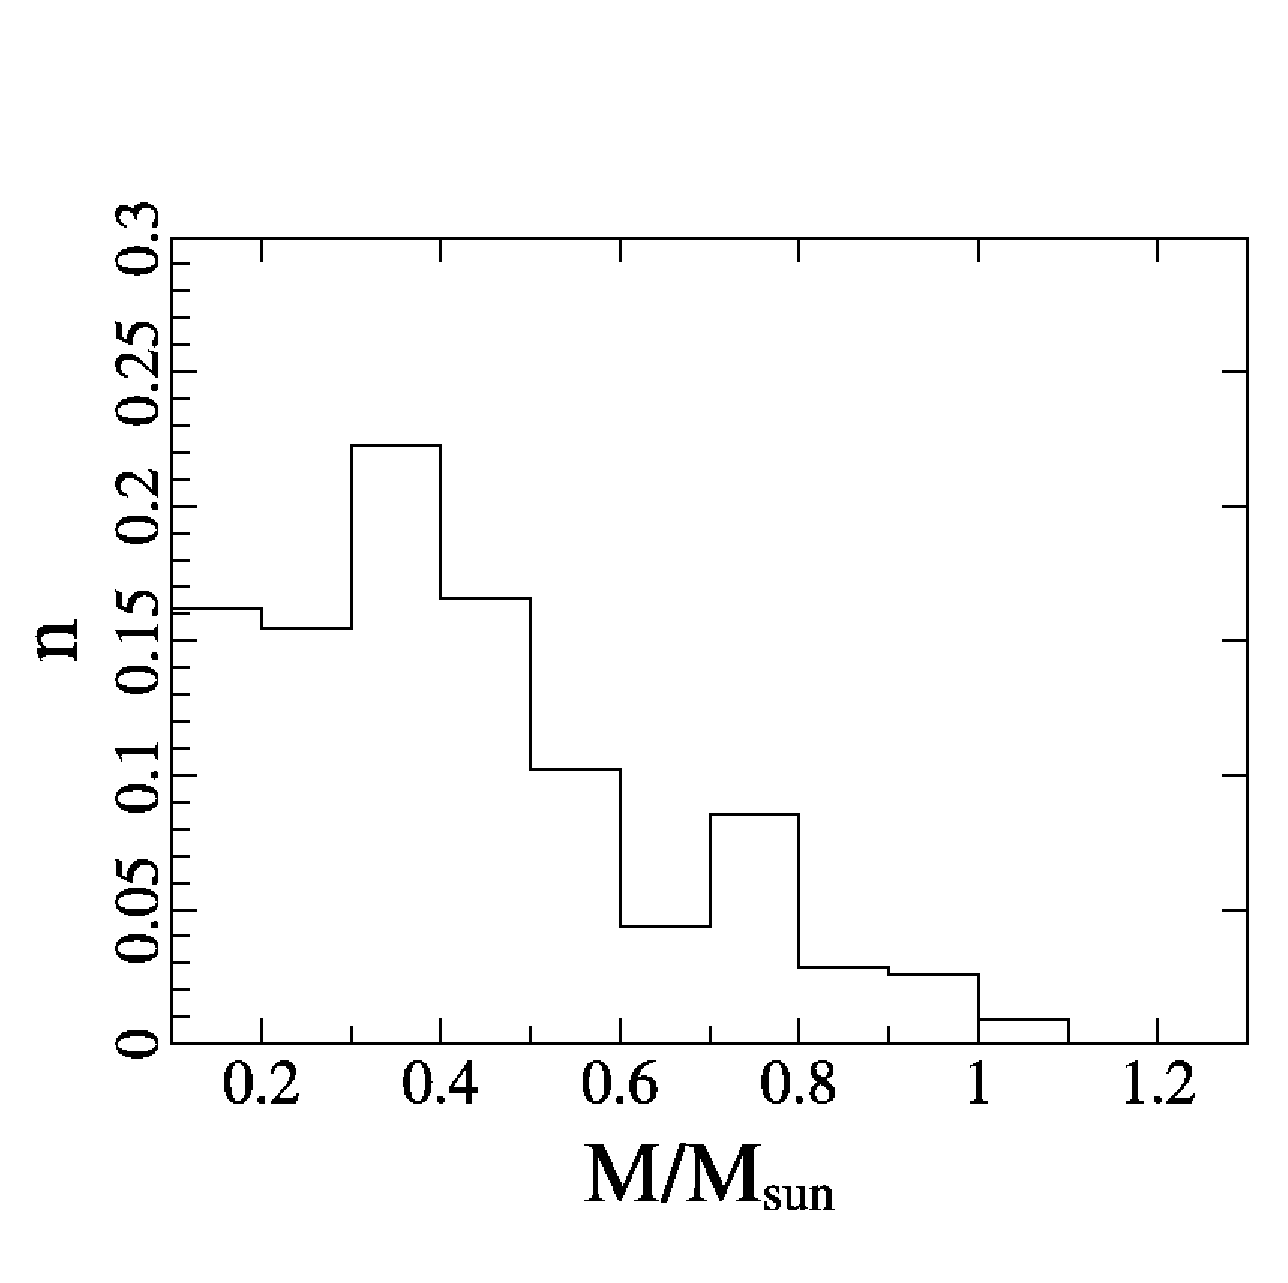
\includegraphics[width=0.4\columnwidth]{fig2d.eps}
\caption{Распределение звезд пулковской программы по величине полного собственного движения (сверху и слева), по звездной величине (сверху и справа), по расстоянию от Солнца (снизу и слева) и по массе (справа и внизу).}
\label{fig:15hist}
\end{figure}

ПЗС-наблюдения также велись с помощью Нормального астрографа Пулковской обсерватории (D = 330~мм, F = 3500~мм) с 2008 по 2015 годы. Они были необходимы чтобы повысить точность определения квазимгновенных собственных движений звезд.  До 2014 года использовалась камера S2C (рабочее поле - $18\times16$~arcmin при масштабе 900~mas/pix). В 2014 и 2015 годах была установлена камера \mbox{SBIG ST-L-11K} (рабочее поле - $35\times23$~arcmin, масштаб - 530~mas/pix). Съемка проводилась при часовых углах $\pm1$~h сериями от 5 до 10 кадров с экспозициями 60 или 120 секунд в зависимости от блеска исследуемой звезды. В ряде случаев для слабых звезд число кадров в серии увеличивалось до 40, чтобы достичь нужной величины соотношения сигнал/шум путем суммирования отдельных кадров.
\subsection{Использование данных цифровых обзоров неба} \label{subsec:ch3/sect2/sub2}
Уже давно в астрономическую практику вошло понятие \glqq виртуальной обсерватории\grqq , когда результаты наблюдений (в том числе и изображения участков неба) доступны с помощью сети Интернет.  Для нашей задачи представляли интерес обзоры неба, содержащие ПЗС-кадры или сканы фотографических пластинок для всего неба или для значительной его части. В данной работе использованы данные обзоров \todo{SDSS~DR12\footnote{\textit{http://dr12.sdss3.org/fields/}} (Алам и др., 2015), 2MASS\footnote{\textit{http://irsa.ipac.caltech.edu/ibe/}} (Кутри и др., 2003), WISE\footnote{\textit{http://irsa.ipac.caltech.edu/applications/wise/}} (Райт и др. 2010) и STScI DSS\footnote{\textit{http://archive.stsci.edu/cgi-bin/dss\_form}} (Ласкер и др., 1998) (сканы пластинок Паломарского обзора неба POSSI-O и POSSII-J)}.

Для всех перечисленных обзоров существует удобный интерфейс, обеспечивающий возможность запроса fits-файлов. Загрузка необходимых данных осуществлялась автоматически с помощью специально созданного приложения и заняла несколько дней из-за большого объема данных обзора WISE (поля в этом обзоре сняты с многочисленными перекрытиями). Для обзора WISE использовались кадры только \glqq холодной\grqq\  части миссии в полосах W1 и W2, чтобы гарантировать приемлемое значение отношения сигнала к шуму для изображений слабых звезд.

\subsection{Определение пиксельных координат} \label{subsec:ch3/sect2/sub3}
Все ПЗС-кадры и сканы пластинок POSS1 и POSS2 анализировались по единой схеме. Для аппроксимации звездных изображений на каждом кадре использовалось shapеlet-разложение /todo{(Massey, Refregier, 2005)}.

Пиксельные координаты фотоцентра звездного изображения варьировались по схеме, приведенной в цитированной выше работе, чтобы гарантировать минимум суммы квадратов невязок. Этот же принцип применялся для автоматического подбора порядка разложения. Типичные примеры результатов аппроксимации изображений сравнительно яркой звезды на кадрах из разных обзоров приведены на рисунке~\ref{fig:15approx}. В целом, методика измерения изображений работает надежно. Некоторые проблемы наблюдались с выбором порядка разложения для кадров SDSS. Судя по структуре распределения невязок, можно предположить, что порядок несколько переоценен. Как показали результаты астрометрических редукций кадров обзора SDSS, это не критично для астрометрических измерений (для звезд c $V_{mag}$=14 сходимость пиксельных координат лежит в пределах 10~mas).

\begin{figure}[h]
\centering
 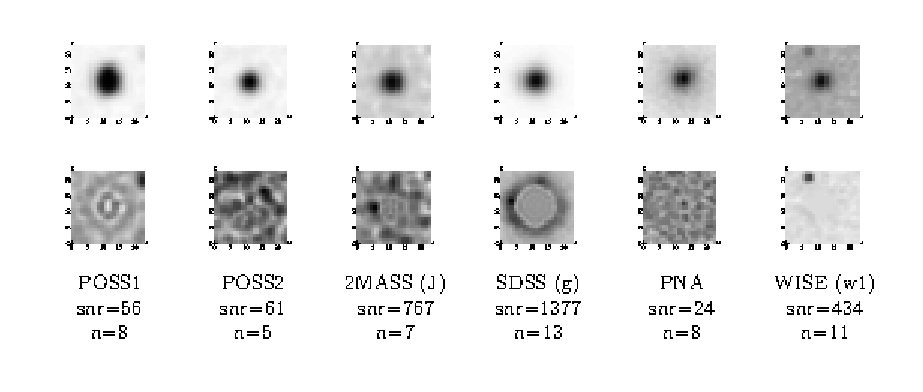
\includegraphics [scale=1] {fig3.eps}
\caption{Аппроксимация изображения звезды J0753+5106 ($V_{mag}$=14.2) на снимках различных обзоров неба. Верхний ряд содержит исходные изображения, нижний "--- результат вычитания \glqq реальное "--- модельное\grqq . Приведены отношение сигнал к шуму для пикселя с максимальным значением отсчета (snr) и порядок shapelet-разложения (n). Размер области изображения $24\times24$~pix.}
\label{fig:15approx}
\end{figure}
\subsection{Анализ систематических ошибок координат звезд в разных обзорах} \label{subsec:ch3/sect2/sub4}
При построении астрометрических каталогов на основе ПЗС-наблюдений часто используется подход, базирующийся на формировании векторных полей остаточных разностей пиксельных координат звезд на основе всего массива данных. Для всех кадров данного обзора была произведена астрометрическая редукция. Постоянные кадра позволили вычислить остаточные разности пиксельных координат опорных звезд \glqq каталог "--- кадр\grqq .

Эти разности могут быть обусловлены комой, дисторсией и другими геометрическими искажениями. Они могут проявлять себя как зависимости невязок от координат и блеска. Примеры таких зависимостей показаны на рисунке~\ref{fig:15posL}. Исходя из приведенных графиков, с большой долей уверенности можно констатировать отсутствие уравнения блеска для пулковских ПЗС-кадров, заметную и сложную дисторсию для кадров космического обзора WISE. Для вычисления поправок рабочее поле кадра разделялось на квадратные (или прямоугольные) области, размеры которых подбирались так, чтобы туда попадало не менее 100 разностей в каждую группу по блеску (от $10^m$ до $16^m$ с шагом $1^m$).

\begin{figure}[h]
\centering
% \includegraphics [scale=1] {fig4.ps}
\includegraphics[width=0.4\columnwidth]{fig4a.eps}
\includegraphics[width=0.4\columnwidth]{fig4b.eps}
\caption{Примеры зависимостей остаточных разностей координат звезд от блеска и положения в кадре. Слева - для пулковских ПЗС-кадров (масштаб - 0.950~arcsec/pix), справа - для изображений WISE (в полосе W1, масштаб - 2.758~arcsec/pix).}
\label{fig:15posL}
\end{figure}

В качестве поправок для геометрического центра области использовались средние величины от всех разностей, попавших в данную ячейку с соответствующими значениями координат центра и звездной величины. Величины поправок для любой точки и значения блеска вычислялись путем бикубической интерполяции. Примеры векторных полей остаточных разностей демонстрируются на рисунке~\ref{fig:15pixL}. Видно, что влияние значительной дисторсии телескопа WISE вполне можно выявить и корректно учесть. Кадры обзора SDSS свободны от значимых геометрических искажений. Уровень систематических ошибок составляет десятые и сотые доли пикселя (менее 40~--~50~mas).

\begin{figure}[h]
\centering
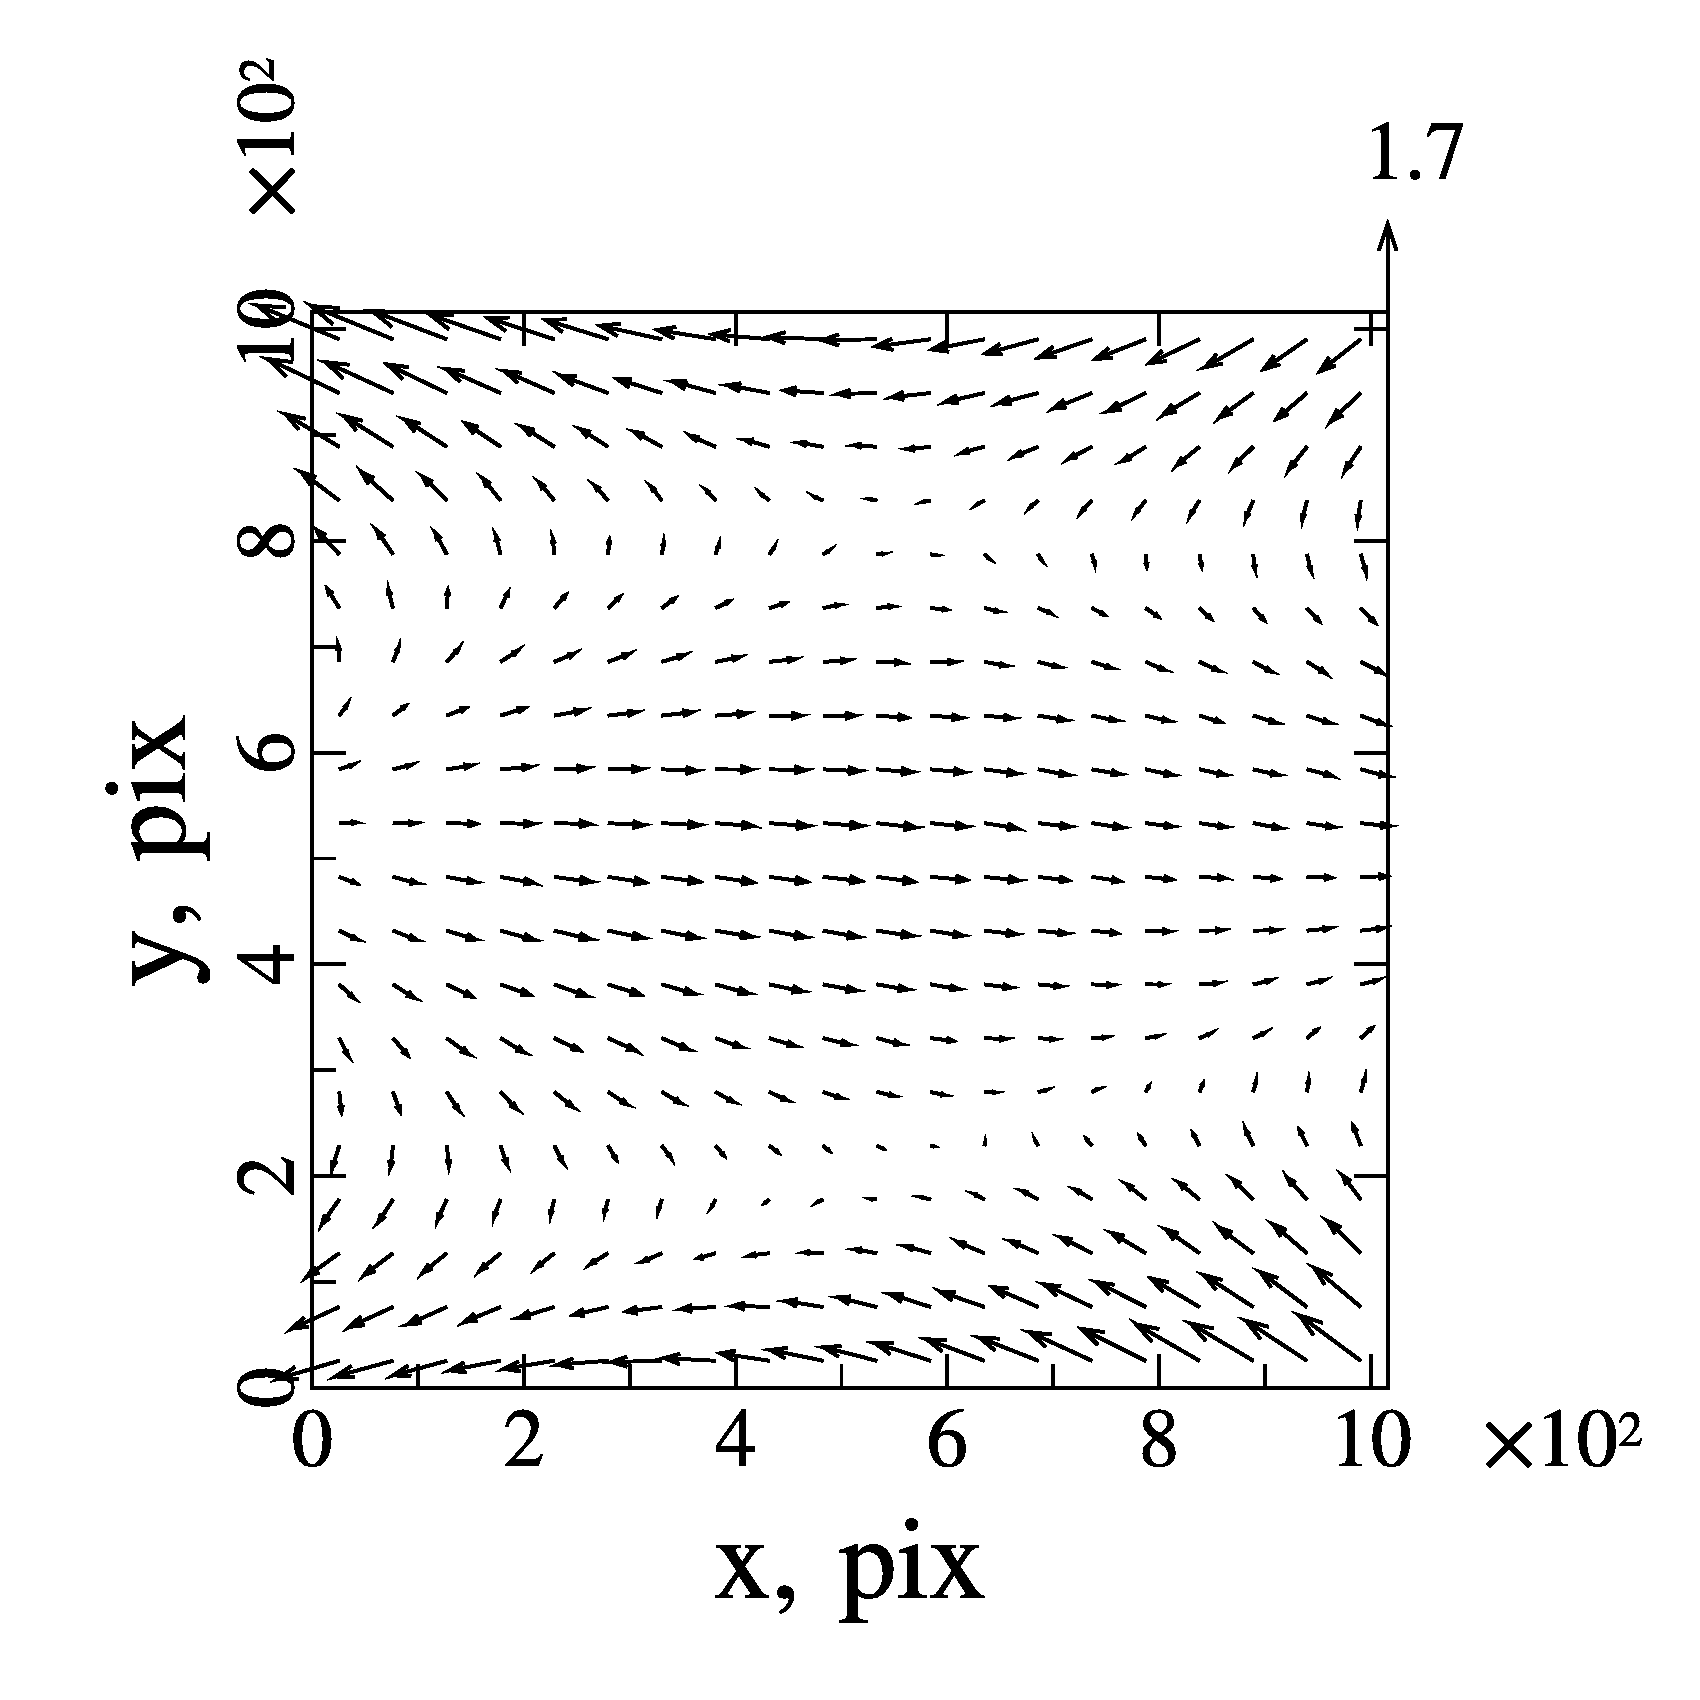
\includegraphics[width=0.4\columnwidth]{fig5a.eps}
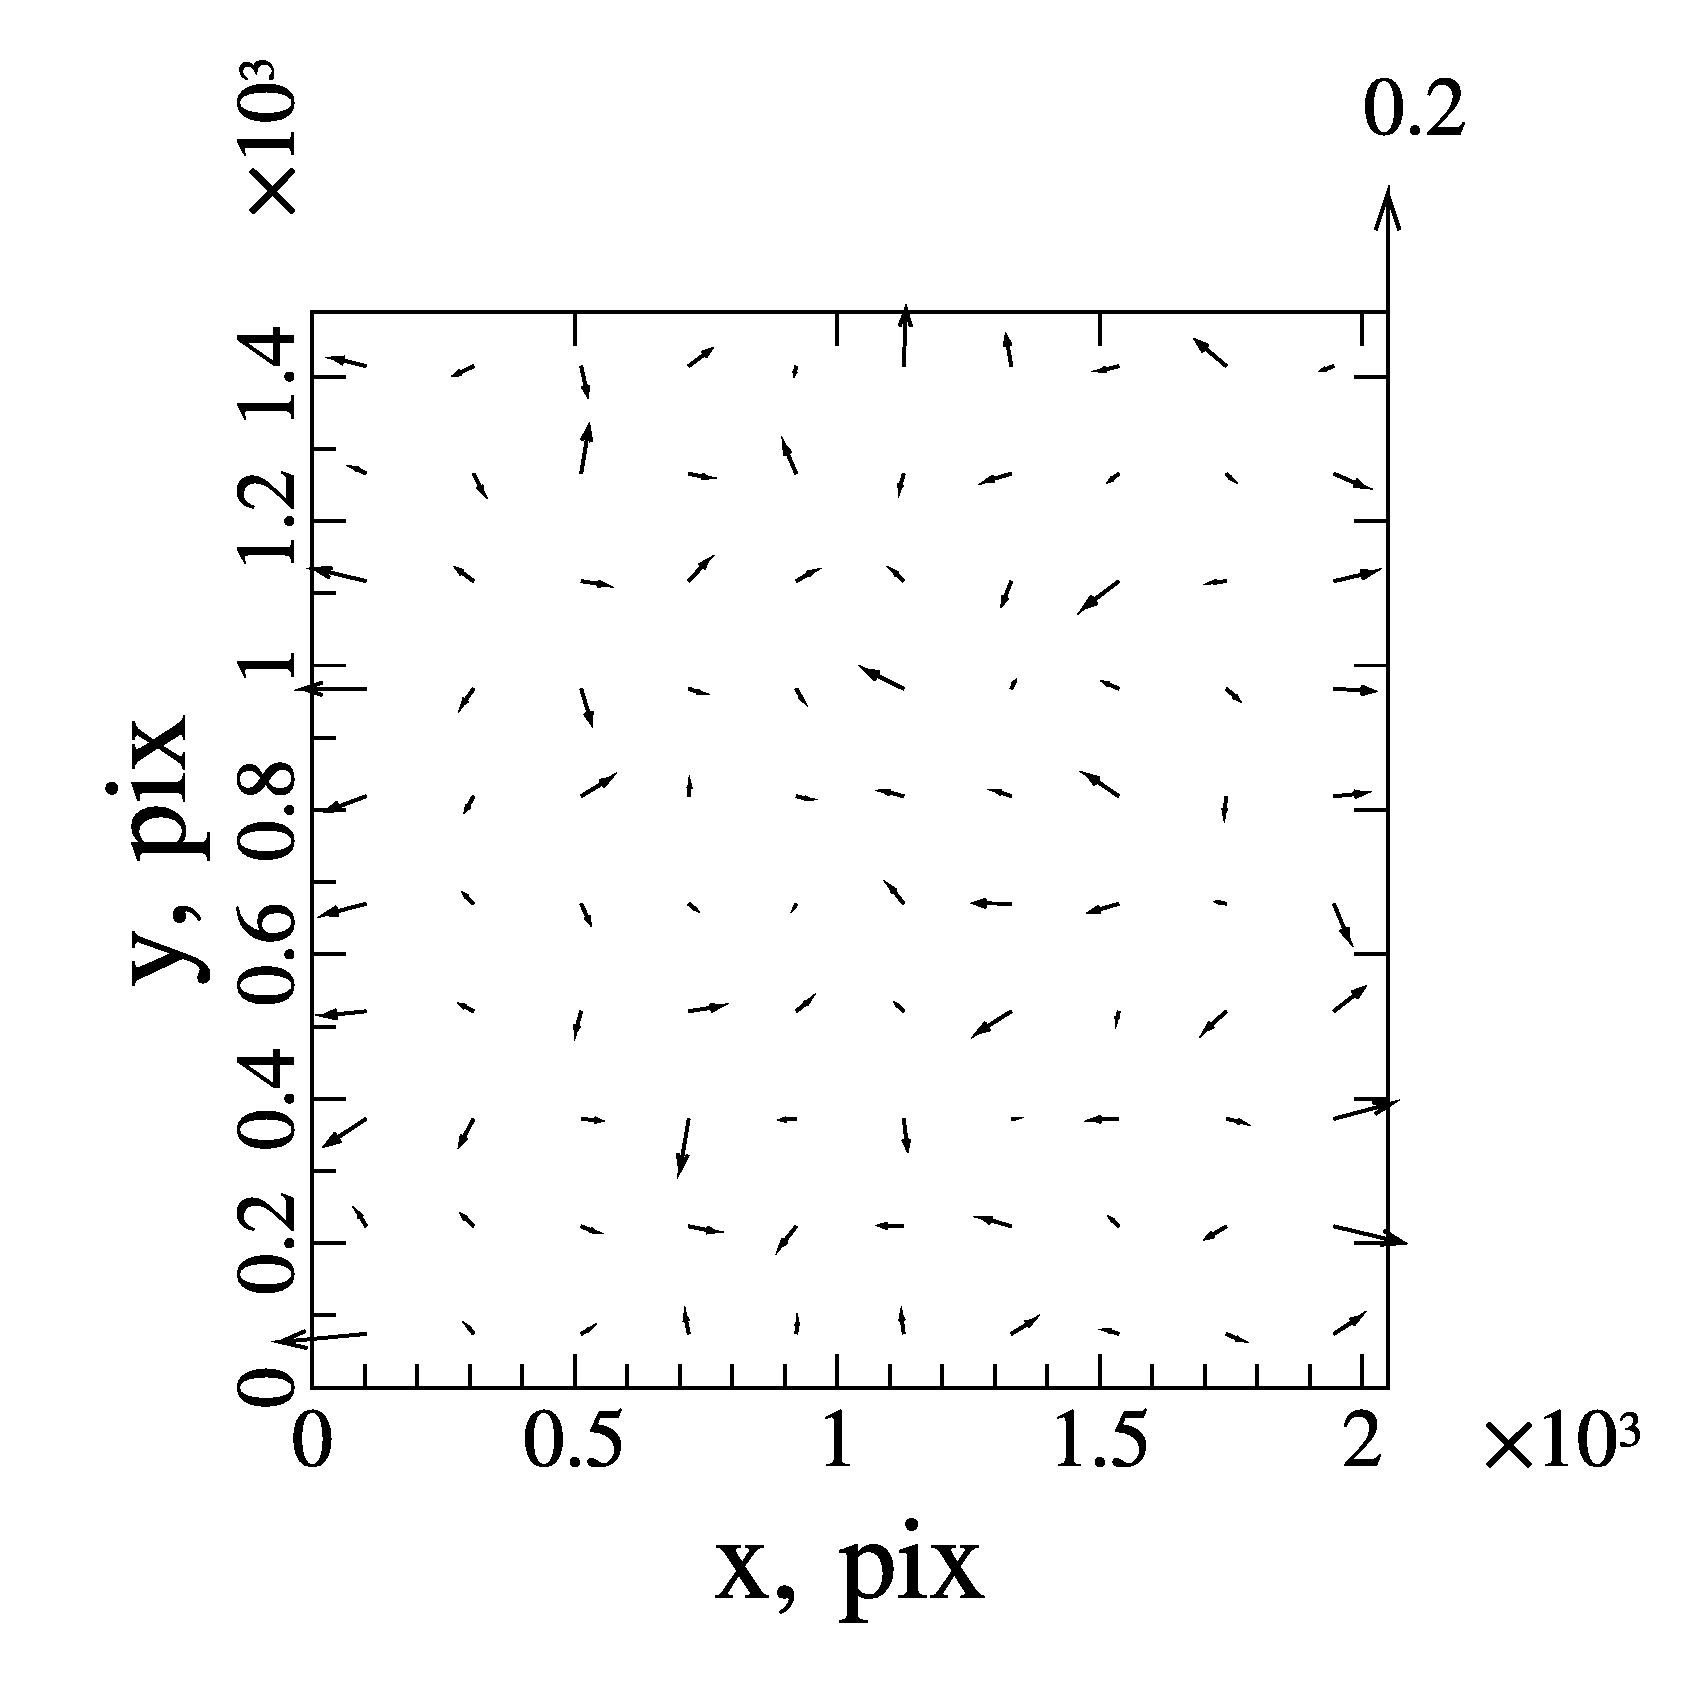
\includegraphics[width=0.4\columnwidth]{fig5b.eps}
\caption{Примеры векторных полей остаточных разностей пиксельных координат звезд в диапазоне $14^m$ -- $16^m$. Слева "--- для всех использованных изображений WISE (в полосе W1, масштаб - 2.758 arcsec/pix). Справа "--- для всех изображений SDSS DR12 (в полосе r, масштаб "--- 0.396~arcsec/pix). В правом верхнем углу изображен максимальный по модулю вектор (его величина указана в pix).}
\label{fig:15pixL}
\end{figure}

Таким образом, для всех используемых обзоров (и для фотометрических полос внутри обзора) были построены карты поправок, позволяющие учесть самые значимые систематические ошибки и получить координаты опорных и определяемых звезд, пригодные для вывода собственных движений.
\section{Выявление $\Delta\mu$--двойных звезд} \label{sec:ch3/sect3}
Для каждой звезды были сформированы наборы кадров из всех возможных обзоров, найдены и измерены общие звезды. Следует заметить, что довольно много областей отсутствуют в SDSS, в ряде случаев изображение программной звезды измерялось неудовлетворительно на кадрах WISE или сканах паломарских пластинок. В качестве опорных выбирались звезды, изображения которых в пикселе с максимальным значением отсчета характеризовались величиной отношения сигнал к шуму snr~>~10 на всех кадрах. Каждая из этих звезд имеет надежно определенное собственное движение в каталоге UCAC4 \todo{(Захариас и др., 2013)}. В пиксельные координаты опорных звезд были внесены соответствующие поправки за систематические ошибки и собственные движения.

В каждом наборе определялся опорный кадр. Момент съемки этого кадра был ближе чем у всех остальных к средней эпохе наблюдений, вычисляемой по всем кадрам. Для каждого кадра методом наименьших квадратов вычислялись параметры линейной модели перехода к опорному кадру. В результате для определяемой звезды получался набор координат в системе опорного кадра.

В использованных обзорах одна и та же область снималась несколько раз (с разными фильтрами). Например, в SDSS было минимум пять кадров для соответствующих фотометрических полос. Для 2MASS и WISE съемка велась как в разных полосах, так и с перекрытием (интересующая нас область присутствовала на нескольких кадрах). В результате появлялась возможность не только повысить точность координат путем взятия среднего, но и оценить точность их определения. Стандартные ошибки положений зависят от используемого обзора. Для SDSS и 2MASS они лежат в пределах 20~--~40~mas, для паломарских обзоров и WISE  - 80~--~150~mas, для пулковских серий ПЗС-кадров внутренняя сходимость определения координат звезд на опорном кадре составляет 50~--~100~mas в зависимости от блеска звезды.

Всего определялось три варианта собственного движения. Первый из них представляет собой результат линейной МНК-аппроксимации движения по всем точкам. Веса точек назначались в зависимости от стандартных ошибок координат звезды для соответствующих эпох. Первые два положения в наборе отвечали средним эпохам POSS1 (1950-е) и POSS2 (в основном 1980-е и 1990-е). Все остальные отвечают более поздним обзорам 2MASS (1998 - 2002), SDSS (2000 - 2015), пулковские кадры (PNA, 2008 - 2015) и WISE (2010, \glqq холодная\grqq\  фаза миссии). Сказанное иллюстрирует диаграмма движения одной из исследуемых звезд, приведенная на рисунке~\ref{fig:15j0838}. Для получения независимых вариантов квазисреднее собственное движение (второй вариант) вычислялось как разность координат POSS2-POSS1, деленная на разность эпох. Последнее решение рассматривалось как квазимгновенное собственное движение (третий вариант). Оно строилось по аналогии с первым вариантом без учета данных POSS1 и POSS2.

\begin{figure}[h]
\centering
 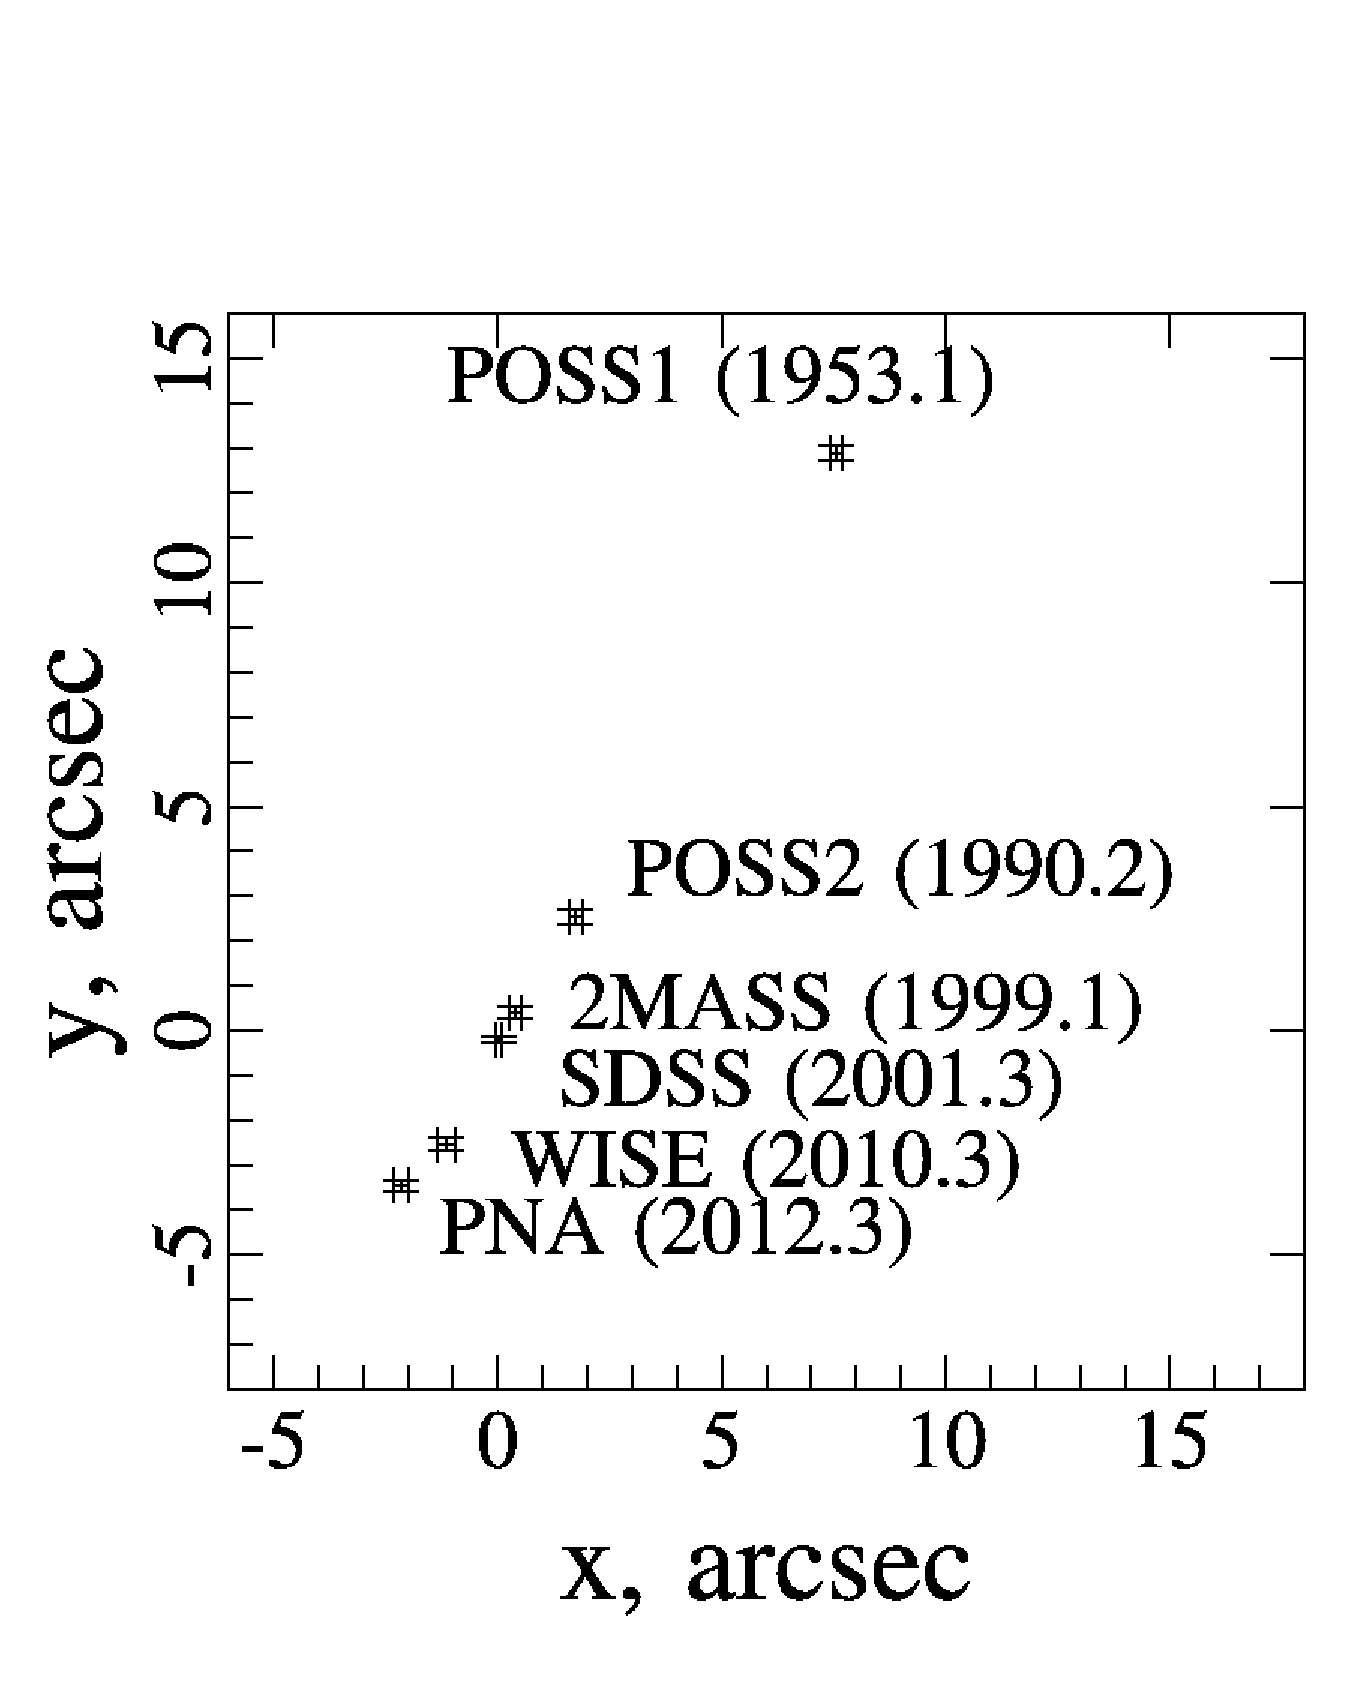
\includegraphics [scale=0.35] {fig6.eps}
\caption{Диаграмма движения звезды J0838+4715. Компоненты собственного движения составляют $-158.1\pm2.6$~mas/год по прямому восхождению и $-273.1\pm3.1$~mas/год по склонению. Средняя эпоха наблюдений - 1994.3328. $V_{mag} = 15.9$ (PNA - Пулковский Нормальный астрограф).}
\label{fig:15j0838}
\end{figure}
\subsection{Вычисление порогового значения критерия для выявления $\Delta\mu$--двойных} \label{subsec:ch3/sect3/sub1}
Как упомянуто в первой главе, в работе Вилена и коллег (Вилен и др., 1999) предложен статистический критерий, позволяющий решить, можно ли считать значимым различие квазисреднего ($\mu_{mean}$) и квазимгновенного ($\mu_{inst}$) собственных движений. В случае данных FK5 и Hipparcos собственные движения определялись на основе большого числа наблюдений, и сомнений в гауссовом характере распределения этих величин не было.

Величина F вычисляется по аналогии с формулой~\ref{eq:KhrF}: $$F^2=\left(\frac{\Delta\mu_\alpha\cos\delta}{\varepsilon_{\mu_\alpha}}\right)^2 + \left(\frac{\Delta\mu_\delta}{\varepsilon_{\mu_\delta}}\right)^2, $$ здесь $\Delta\mu_\alpha\cos\delta,~\Delta\mu_\delta$ - разности компонент собственного движения ($\mu_{mean}-\mu_{inst}$); $\varepsilon_{\mu_\alpha},~\varepsilon_{\mu_\delta}$ - соответствующие взаимные стандартные ошибки ($\varepsilon_\mu^2=\varepsilon_{\mu_{inst}}^2+\varepsilon_{\mu_{mean}}^2$).

Анализ интегрального распределения этой величины приводит к выводу, что при F>2.49 вероятность наблюдения соответствующих разностей собственных движений для одиночных звезд меньше 0.05. Именно такие звезды рассматривались в работе Вилена и коллег (Вилен и др., 1999) как кандидаты в $\Delta\mu$-двойные.

В нашем случае количество точек, по которым необходимо сделать вывод, невелико (от 4 до 10). Поэтому необходимо было проверить, можно ли использовать значение F=2.49 как пороговое. Для этого было предпринято численное моделирование линейного движения одиночной звезды по небесной сфере с заданными ошибками определения координат, охватывающего характерный для нашей задачи период времени (около 65 лет). Точки для определения собственных движений брались случайным образом, учитывая характерные времена осуществления используемых обзоров. Далее производились вычисления по схеме, описанной в предыдущем разделе, но для модельной звезды.

Рассматривались разные случаи: от 4 точек (есть два паломарских снимка, пулковские кадры и кадры 2MASS) до 10. Для каждого производилось 100000 испытаний. В результате для каждого случая строилось интегральное распределение величины F и вычислялось пороговое значение.

Как видно из графика на рисунке~\ref{fig:15Fint}, для 6 точек $F>5.3$, для 10 “--- $F>3.1$ и так далее. При увеличении до 20 точек пороговое приближается к 2.5. Что соответствует ситуации, рассмотренной в работе Вилена и коллег. Полученные таким образом пороговые значения использовались для реальных звезд, чтобы сделать вывод о характере движения звезды по небесной сфере.

\begin{figure}[h]
\centering
%\includegraphics [scale=1] {fig7.ps}
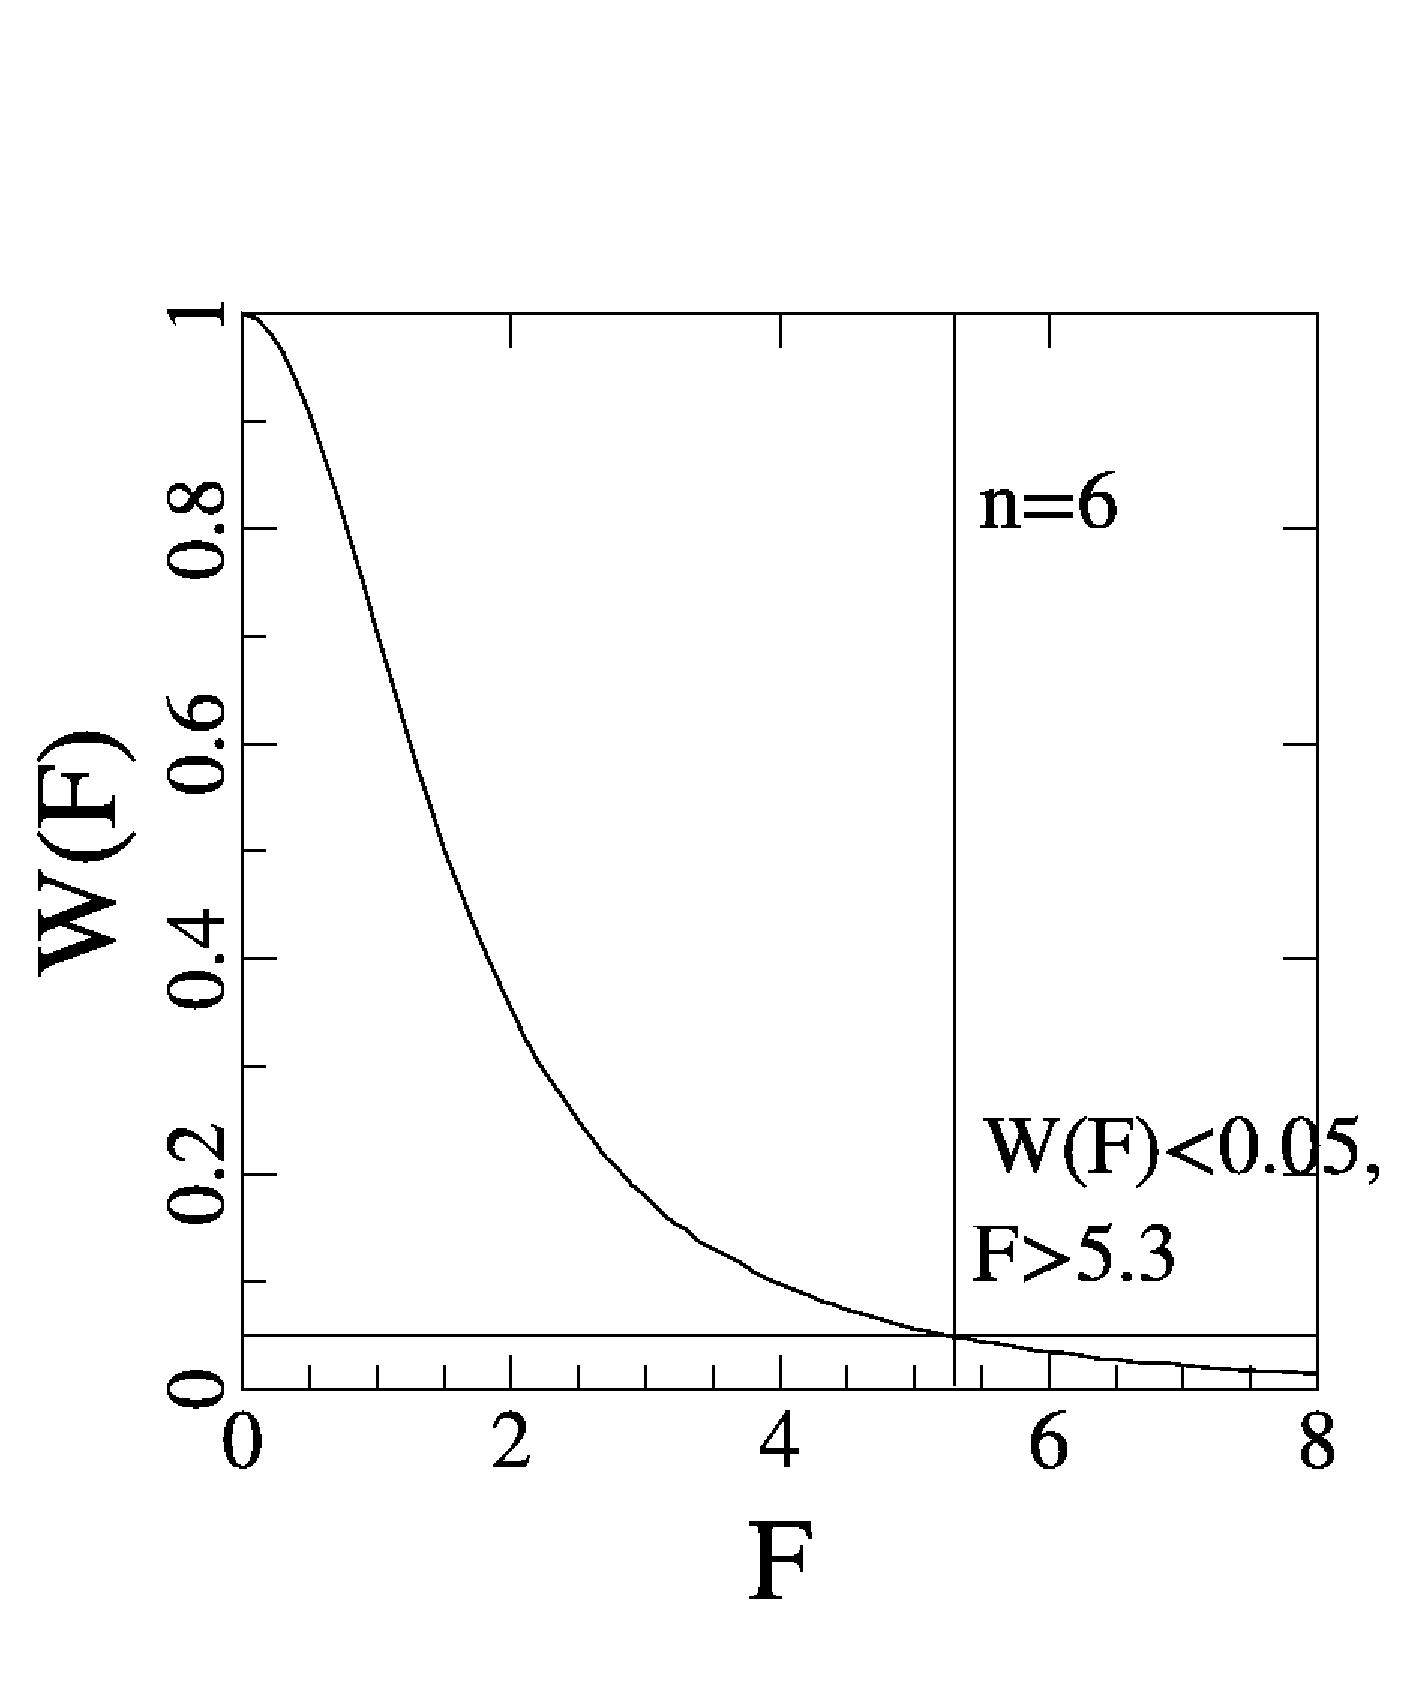
\includegraphics[width=0.4\columnwidth]{fig7a.eps}
\includegraphics[width=0.4\columnwidth]{fig7b.eps}
\caption{Интегральные распределения величины F для разного числа кадров, использованных для вычисления собственных движений (слева n=6, справа n=10).}
\label{fig:15Fint}
\end{figure}
\subsection{Общая характеристика полученных собственных движений} \label{subsec:ch3/sect3/sub2}
В конечном итоге с использованием описанной методики были обработаны кадры и сканы фотопластинок для 1308 звезд. Положения 120 звезд не удалось надежно измерить на кадрах ряда обзоров чаще всего из-за наличия рядом изображений очень ярких звезд. Для этих объектов требуются дополнительные исследования.

Все результаты образованы 4 таблицы, доступные в электронном виде в базе данных \todo{CDS (http://vizier.u-strasbg.fr/viz-bin/VizieR?-source=J/PAZh/41/896)}. В качестве примера, небольшая часть основного массива данных показана в таблице~\ref{tab:candidates}. Для каждой звезды помимо собственных движений и оценок F-критерия, вычисленных в данной работе, приводятся дополнительные данные (разности собственных движений из сравнения с данными LSPM, фотометрические и тригонометрические параллаксы, оценки блеска для разных полос, принадлежность к каталогам двойных звезд). При формировании таблиц использовался сервис Центра астрономических данных в Страсбурге (Centre de Donnees astronomiques de Strasbourg) \todo{(Ошенбейн и др., 2000)}.

Надежность определения квазимгновенных собственных движений (третий вариант) существенно зависит от разности эпох между обзорами. Поэтому материал был разделен на две части. В первую из них вошли звезды, с соответствующей разностью эпох более 5~лет, все остальные “--- во вторую. В первой части оказалось 944 звезды, для которых не обнаружены признаки нелинейности движения, и 121 звезда, проявляющая себя как кандидат в $\Delta\mu$-двойные. Вторую группу составили 229 одиночных звезд  и 14 звезд-кандидатов в $\Delta\mu$-двойные.

Для собственных движений, построенных по всем обзорам (первый вариант), средняя точность составила чуть хуже 4~mas/год по обеим координатам. Для более полного представления о качестве собственных движений на рисунке~\ref{fig:15emu} приведены соответствующие гистограмма и зависимость ошибок определения собственных движений от блеска (для первого варианта собственных движений). Для подавляющего числа звезд ошибки определения собственных движений не превосходят 10~mas/год.

\begin{figure}[h]
\centering
%\includegraphics [scale=1] {fig8.ps}
\includegraphics[width=0.4\columnwidth]{fig8a.eps}
\includegraphics[width=0.4\columnwidth]{fig8b.eps}
\caption{Распределение ошибок собственных движений (слева) и их зависимость от блеска (справа).}
\label{fig:15emu}
\end{figure}

квазисредние собственные движения характеризуются средней точностью около 5~--~10~mas/год. Для квазимгновенных собственных движений эта величина составила 10~--~20~mas/год (она существенно зависит от наличия кадров SDSS и блеска звезды).

Наличие систематических различий между нашим набором собственных движений и собственными движениями звезд в каталоге LSPM демонстрирует рисунок~\ref{fig:15dmu}. Особенно эти различия заметны для собственных движений по склонению (разности могут достигать величины 2~--~4~mas/год).
\begin{figure}[h]
\centering
%\includegraphics [scale=1] {fig9.ps}
\includegraphics[width=0.4\columnwidth]{fig9a.eps}
\includegraphics[width=0.4\columnwidth]{fig9b.eps}
\caption{Зависимость разностей собственных движений $\mu - \mu_{LSPM}$ от звездной величины ($\mu$ - собственное движение, вычисленное по всем кадрам).}
\label{fig:15dmu}
\end{figure}
Особенность каталога LSPM состоит в нестандартном подходе к абсолютизации собственных движений. В период его создания слабые опорные звезды еще не были обеспечены надежными собственными движениями. Поэтому эта процедура производилась по ярким звездам каталога Tycho-2, изображения которых на пластинках паломарских обзоров либо передержаны, либо близки к этому. Экстраполяция абсолютизирующих поправок в область более слабых (на $3^m~--~5^m$) звезд никак не контролировалась, что, вероятно, стало причиной наблюдаемых систематических различий.
\subsection{Верификация выявленных звезд-кандидатов в $\Delta\mu$-двойные} \label{subsec:ch3/sect3/sub3}
Всего у 121 объекта обнаруживаются признаки нелинейности движения по небесной сфере, что классифицирует такие звезды как $\Delta\mu$-двойные. На наш взгляд, эти объекты представляют интерес для дальнейших исследований с целью подтверждения факта двойственности и определения орбит и масс посредством, например,  спекл-интерферометрических наблюдений на больших телескопах. Для 14 звезд из второй группы, для которых квазимгновенное собственное движение заметно отличается от квазисреднего, вывод о принадлежности к $\Delta\mu$-двойным представляется весьма ненадежным из-за малости разности эпох между положениями в современных обзорах неба. Поэтому дальнейший анализ касается только звезд первой группы.

Из нашего списка $\Delta\mu$-двойных 10 звезд входят в состав каталога WDS \todo{(Мейсон и др., 2001)}, то есть являются визуально-двойными звездами (это 9\% от общего числа $\Delta\mu$-двойных звезд). Большинство из них представляют собой широкие пары звезд с общим собственным движением (угловое разделение компонент составляет десятки угловых секунд, а в ряде случаев и минуты дуги). Данный результат является слабым подтверждением эффективности методики выявления $\Delta\mu$-двойных звезд. В списке из 944 \glqq одиночных\grqq\ звезд присутствует 58 вхождений в WDS (6\,\%). Поэтому нельзя говорить, что в списке  $\Delta\mu$--двойных доля известных визуально-двойных звезд значимо больше.

Часть звезд пулковской программы имеет тригонометрические параллаксы, полученные по наземным наблюдениям. Хорошо известно, что в ходе таких наблюдений совместно с параллаксами с высокой точностью определяются и величины собственных движений за короткий интервал времени (3~--~5 лет). Поэтому их можно рассматривать как квазимгновенные собственные движения и оценить величину $F_{\pi}$ из сравнения с собственным движением, определенным по итогам данной работы.

В нашем списке $\Delta\mu$-двойных оказалось 33 звезды, вошедших в параллактические программы. Из них 18 имеют величину $F_{\pi}>3$ (и пять звезд входят в WDS). Более детально о корреляции между независимыми наборами величин $F$ и $F_\pi$ можно судить по рисунку~\ref{fig:15FF}. С некоторой натяжкой можно говорить о наличии корреляции между $F$ и $F_\pi$ для $\Delta\mu$-двойных. В случае звезд, которые рассматриваются как \glqq одиночные\grqq\ признаки корреляции не столь заметны. Положения визуально-двойных звезд из каталога WDS помечены на рисунке~\ref{fig:15FF} незакрашенными символами. Они есть как среди $\Delta\mu$-двойных, так и в числе \glqq одиночных\grqq\ звезд. И это вполне естественно. Для широких пар с большими периодами обращения (сотни и тысячи лет), которых довольно много в нашем материале, орбитальное движение очень непросто обнаружить на используемом ряде наблюдений.
\begin{figure}[h]
\centering
 \includegraphics [scale=0.35] {fig10.eps}
\caption{Распределение звезд на плоскости $F-F_{\pi}$. $F$ - значения критерия, полученные из анализа ПЗС-кадров и сканов обзоров. $F_{\pi}$ определялись на основе собственных движений из данной работы и собственных движений, полученных в ходе реализации различных параллактических программ (кружки обозначают `одиночные' звезды, квадраты -  $\Delta\mu$-двойные; символы, отвечающие звездам из каталога WDS, не закрашены)}
\label{fig:15FF}
\end{figure}
Для близких к Солнцу двойных систем карликовых звезд угловые расстояния между компонентами могут составлять секунду дуги и более. Поэтому факт двойственности может быть установлен просто из анализа изображений звезд на ПЗС-кадрах. Shapelet--разложение, использованное для определения пиксельных координат звезд, позволяет оценивать такой параметр как асимметрия изображения. Для того, чтобы понять насколько надежен такой подход, было выполнено численное моделирование изображений подобных пар. Для обзора SDSS, который обладает наилучшим \glqq разрешением\grqq\ среди всех использованных обзоров, на основе результатов аппроксимации изображений одиночных звезд строились модельные \glqq взаимодействующие\grqq\ изображения для систем с характерными значениями блеска компонент при разных угловых расстояниях между ними. Затем эти \glqq взаимодействующие\grqq\ изображения снова подвергалось Shapelet-разложению. Пример зависимости асимметрии от углового расстояния для пары с блеском компонент $14.1^m$ и $15.3^m$ показан на рисунке~\ref{fig:15asimm}. Анализ этого графика дает основания говорить, что оценки асимметрии изображений наиболее эффективны для угловых расстояний 2~--~4 угловых секунды. Асимметрия заметна и для меньших разделений, но для оценки надежности рассматриваемого подхода для таких \glqq тесных пар\grqq\ требуются дополнительные исследования. Учитывая качество изображений и масштабы ПЗС-кадров и сканов из остальных использованных обзоров можно заключить, что оценок асимметрии изображений недостаточно для установления факта двойственности. Тем не менее, величины асимметрии весьма информативны для анализа вместе с оценками F--критерия. Поэтому в финальную таблицу с результатами включены средние величины асимметрии по всем обзорам, приведены максимальные величины асимметрии по всей выборке для данной звезды с указанием соответствующего обзора (таблица~\ref{tab:candidates}). Любопытно отметить, что для выборки $\Delta\mu$--двойных звезд средняя асимметрия звездных изображений составляет 0.039. Для \glqq одиночных\grqq\ звезд этот показатель составил 0.025.
\begin{figure}[h]
\centering
 \includegraphics [scale=0.35] {fig11.eps}
\caption{Симуляция зависимости асимметрии взаимодействующих изображений звезд от углового расстояния между звездами (главная компонента - $14.1^m$, вторая звезда - $15.3^m$). За основу были взяты результаты shapelet--разложений звезд на кадрах обзора SDSS.}
\label{fig:15asimm}
\end{figure}
Параметры двойных систем из каталога WDS (разделение между компонентами, позиционные углы, блеск компонент) включены в электронные версии таблиц с результатами. Для $\Delta\mu$--двойных звезд J0027+5330N, J0514+4431N, J0517+4550, J1614+6038, J1938+3512E угловые разделения между компонентами лежат в пределах от долей угловой секунды до $4''$. Звезда J1938+3512E входит в обзор SDSS и имеет асимметрию 0.086, что заметно выше средних показателей для \glqq одиночных\grqq\ звезд того же блеска в этом обзоре (обычно от 0 до 0.04). Эти звезды можно выделить как примеры успешного детектирования нелинейного движения по небесной сфере на основе сравнения квазисреднего и квазимгновенного собственных движений.

Положения фотоцентров изображений рассматриваемых двойных систем могут отличаться в зависимости от эффективной длины волны в случае заметной разности эффективных температур компонент (например, для систем типа \glqq М--карлик + коричневый карлик'). Если бы обзоры выполнялись одновременно, можно было бы легко обнаружить этот факт, сравнивая координаты звезд и выделяя заметные смещения центров изображений от \glqq оптических\grqq\ к \glqq инфракрасным\grqq\ обзорам. Космический обзор WISE более современный и более глубокий по сравнению с 2MASS. Но в астрометрическом отношении обзор 2MASS значительно более качественный (ошибки астрометрической редукции для WISE могут достигать 100~--~200~mas, для 2MASS они, как правило, меньше 50~mas). Поэтому если число положений звезды в \glqq оптических\grqq\ обзорах (POSS1, POSS2, SDSS, PNA) было не менее четырех, вычислялся вариант собственного движения только по данным \glqq оптических\grqq\ обзоров. С помощью этого собственного движения вычислялось \glqq оптическое\grqq\ положение звезды на эпоху обзора 2MASS. В результате можно было оценить смещение ($\rho$) между \glqq оптическим\grqq\ положением и положением в обзоре 2MASS. Если $\rho>5\sigma$, величина смещения и его отношение к взаимной ошибке координат приводится в финальной таблице. Например, звезда J1931+4115 (таблица~\ref{tab:candidates}). Для нее смещение превосходит $1''$. Асимметрия изображения для этой звезды близка к средней по выборке $\Delta\mu$-двойных звезд и больше средней для \glqq одиночных\grqq . Такой совместный анализ множества критериев позволяет заключить, что предложенная методика поиска $\Delta\mu$-двойных звезд является эффективной для определенного класса двойных систем среди звезд низкой светимости.

Еще одна возможность верификации детектирования $\Delta\mu$-двойных связана с анализом фотометрических данных. Самые точные из доступных для выявленных звезд оценок блеска присутствуют в SDSS (это величины u,g,r,i,z). Используя безансонскую модель Галактики \todo{(Робин и др., 2003)} и падуанские изохроны\footnote{\textit{http://stev.oapd.inaf.it/cgi-bin/cmd}} \todo{(Брессан и др., 2012; Чен и др., 2014; Танг и др., 2015)}, были построены двухцветные диаграммы (g-z)~--~(u-g) для звезд с массами от 0.1 до 0.7 массы Солнца. Техника построения диаграмм полностью аналогична методике, ранее использованной при реализации пулковской программы изучения звезд с большими собственными движениями \todo{(Ховричев и др. 2013)}.

Чтобы понять, как смешение цветов неразрешенных звездных пар влияет на распределение плотности, с которой звезды заполняют пространство (g-z)~--~(u-g), строились диаграммы как для одиночных звезд, так и с учетом различных комбинаций компонент двойных систем в зависимости от масс и возрастов (при этом считалось, что доля двойных звезд составляет 0.5).  Положения выявленных звезд-кандидатов в $\Delta\mu$-двойные на диаграммах для одиночных (слева) и с учетом доли двойных звезд (справа) показаны на рисунке~\ref{fig:15color}.
\begin{figure}[h]
\centering
%\includegraphics [scale=1] {fig12.ps}
\includegraphics[width=0.4\columnwidth]{fig12a.eps}
\includegraphics[width=0.4\columnwidth]{fig12b.eps}
\caption{Положения звед-кандидатов в $\Delta\mu$-двойные на двухцветной диаграмме $(g-z)$~--~$(u-g)$. На рисунке показаны теоретические последовательности для звезд в диапазоне от 0.1 до 0.7 массы Солнца, построенные на основе падуанских изохрон и безансонской модели Галактики для одиночных звезд (слева) и при добавлении двойных систем типа  \glqq M--карлик + белый карлик\grqq  (справа). Массы белых карликов составляют 0.3 и 0.6 массы Солнца (возрасты 0.6 и 1 млрд. лет соответственно). Черные квадраты соответствуют звездам, которые могут оказаться системами  \glqq M-карлик + белый карлик\grqq . Шкала справа показывает значение натурального логарифма относительной плотности распределения модельных звезд на диаграмме.}
\label{fig:15color}
\end{figure}
Метод поиска $\Delta\mu$-двойных максимально эффективен при большом различии положений центра масс и фотоцентра двойной системы. Поэтому большой интерес вызывает поиск пар \glqq M--карлик + белый карлик\grqq , для которых отношение светимостей компонент заметно больше отношения масс. Модельные расчеты показали, что для большинства комбинаций M-карликов разных масс отклонения от основного массива точек на диаграмме (g-z)~--~(u-g) незаметны. В то время как пары \glqq M-карлик + белый карлик\grqq\ могут дать заметный эффект. Чтобы оценить его наглядно, для примера, были взяты модели белых карликов  с массами 0.3 и 0.6 массы Солнца и возрастами 0.6 и 1 млрд. лет \todo{(Хольберг и Бержерон, 2006; Бержерон и др., 2011; Ковальски и Саумон, 2006; Тремблей и др., 2011)}\footnote{\textit{http://www.astro.umontreal.ca/~bergeron/CoolingModels/}}. Смешение цветов данных белых карликов с цветами M-карликов разных масс и соответствующих возрастов (с учетом того, что белые карлики прошли прошли фазу эволюции на главной последовательности) обуславливает отличие вида диаграмм на левой и правой панелях рисунка~\ref{fig:15color}.  Анализ отклонений $\Delta\mu$--двойных от основного массива точек на этом рисунке дает основания для вывода о том, что 4 звезды (J0656+3827, J0838+3940, J1229+5332, J2330+4639 - обозначены квадратными метками) могут рассматриваться как возможные пары такого типа.

Подробная информация об этих четырех звездах приведена в таблице~\ref{tab:MDWD}. Три звезды из четырех характеризуются большими ($>0.1$) значениями асимметрии звездных изображений, полученными при анализе ПЗС-кадров обзора SDSS. Привлекает внимание звезда J2330+4639, входящая в WDS как сравнительно широкая пара (разделение компонент 21.4~arcsec). Для этой звезды очень сильно отличаются квазимгновенные и квазисредние собственные движения при очень большой асимметрии (0.244). Это можно объяснить как следствие \glqq взаимодействия\grqq\ изображений двух близко расположенных звезд, что могло стать причиной систематической ошибки определения координат звезды в одном из современных обзоров. При анализе этой информации следует иметь ввиду, что в плотных звездных полях (когда на небольшом участке кадра в несколько минут дуги наблюдаются десятки звезд) близкие к Солнцу и быстро летящие звезды способны располагаться очень тесно к звездам фона на кадрах отдельных обзоров. Поэтому возможно формирование \glqq взаимодействующих\grqq\ изображений в ситуации, когда речь не может идти о двойной звезде. Однако проверить это пока довольно сложно, из-за того, что использованные обзоры имеют разную предельную звездную величину.

Итак, материал этой главы демонстрирует, что метод детектирования $\Delta\mu$-двойных, разработанный изначально для анализа звезд с \glqq хорошей\grqq\ астрометрической историей, был модифицирован для исследвоания собственных движений объектов, имеющих лишь несколько надежных положений. Это позволило установить, что более 100 звезд, относящихся к категории маломассивных карликов солнечной окрестности, могут рассматриваться как кандидаты в двойные системы. Это позволяет более адресно организовать проверку факта двойственности с помощью методов высокого разрешения. Как было показано, рационально принимать во внимание не только факт значимых различий собственных движений, но и свойства изображений звезд на ПЗС-кадрах (из формы). Этот подход будет более подробно изложен в дальнейшем тексте.

\begin{table}[htbp]
%\vspace{6mm}
%\small
\centering
\caption{Фрагменты таблицы для звезд-кандидатов в $\Delta\mu$--двойные.}
\label{tab:candidates}
\vspace{5mm}
\begin{tabularx}{\textwidth}{l|r|r|r|r|r|r|r|r|l} \hline
           & \multicolumn{4}{c|}{Квазисреднее $\mu$ } & \multicolumn{4}{c|}{Квазимгновенное $\mu$}& \\ \cline{2-9}
\multicolumn{1}{c|}{LSPM}&\multicolumn{1}{c|}{$\mu_\alpha$}&\multicolumn{1}{c|}{$\mu_\delta$}&\multicolumn{1}{c|}{$\varepsilon_{\mu_\alpha}$}&\multicolumn{1}{c|}{$\varepsilon_{\mu_\delta}$}&\multicolumn{1}{c|}{$\mu_\alpha$}&\multicolumn{1}{c|}{$\mu_\delta$}&\multicolumn{1}{c|}{$\varepsilon_{\mu_\alpha}$}&\multicolumn{1}{c|}{$\varepsilon_{\mu_\delta}$}&\multicolumn{1}{c}{T}\\ \cline{2-9}	   
	       &\multicolumn{8}{c|}{mas/yr}&\\ \hline  
J1756+5132 & -526.8&  205.3&  5.3&  5.2& -457.7&  -19.4& 17.1& 18.2& 2007.0035\\
J1844+6511 &  -16.5&  356.4&  7.1&  5.4&   30.0&  289.0&  0.3&  3.7& 2005.4087\\
J1908+3216 & -238.5& -227.0&  6.8&  6.3& -200.9& -215.4&  0.5&  9.5& 2006.9105\\
J1931+4115 & -249.7& -119.4& 15.6& 14.1& -329.5&   -1.4&  7.9&  4.4& 2007.7614\\
J1931+6843 &  256.2&  461.7&  6.3&  4.9&  228.9&  349.9&  5.8&  0.4& 2006.9060\\
J1938+3512E&   -2.1&  814.7& 11.4& 12.2& -123.3&  714.9&  6.1&  0.3& 2004.6930\\ \hline
\end{tabularx}
\begin{tabularx}{\textwidth}{l|r|c|r|r|r|r|r|r|l}

\multicolumn{1}{c|}{LSPM}&\multicolumn{1}{c|}{F}&\multicolumn{1}{c|}{n}&\multicolumn{1}{c|}{$V_{mag}$}&\multicolumn{1}{c|}{{\small$V$--$J$}}&\multicolumn{1}{c|}{$\rho$,mas}&\multicolumn{1}{c|}{$\rho/\varepsilon$}&\multicolumn{1}{c|}{$\langle A\rangle\ $}&\multicolumn{1}{c|}{$A_{max}$}& \multicolumn{1}{c}{Обзор}\\ \hline
        J1756+5132 & 12.50& 4 & 15.96& 3.18 &     &     & 0.040& 0.080& poss1\\
J1844+6511 & 12.23& 5 & 16.46& 4.08 &     &     & 0.026& 0.060& poss2\\
J1908+3216 &  5.57& 6 & 11.83& 3.92 &     &     & 0.019& 0.045& wise\\
J1931+4115 &  9.18& 7 & 12.20& 2.12 & 1241&  5.7& 0.032& 0.080& poss2\\
J1931+6843 & 22.90& 5 & 14.67& 4.65 &     &     & 0.027& 0.050& poss1\\
J1938+3512E& 12.44& 5 & 14.75& 2.98 &     &     & 0.038& 0.086& sdss\\
\hline
\end{tabularx}
\begin{flushleft}
\footnotesize
\textbf{Примечание.} $\mu_{\alpha}$, $\mu_{\delta}$, $\varepsilon_{\mu_{\alpha}}$, $\varepsilon_{\mu_{\delta}}$ "--- компоненты собственного движения и их стандартные ошибки.\\T "--- средняя эпоха для квазимгновенного собственного движения.\\F "--- величина критерия \glqq нелинейности\grqq\ движения звезды.\\ n "--- число использованных обзоров.\\ $V_{mag}$, {\small$V$--$J$} "--- звездная величина и показатель цвета. \\ $\rho$ "--- угловое расстояние между \glqq оптическими\grqq\ и \glqq ИК\grqq\ положениями фотоцентра. \\ $\rho/\varepsilon$ "--- отношение $\rho$ к стандартной ошибке ($\varepsilon$) определения координат звезды. \\ $\rho$ и $\rho/\varepsilon$ приводятся, только если $\rho/\varepsilon>5$. \\ $\langle A\rangle\ $"--- среднее значение \glqq асимметрии\grqq\ изображения звезды по всем обзорам. \\ $A_{max}$ "--- максимальное значение \glqq асимметрии\grqq\ изображения звезды и название соответствующего обзора. \\ Звезда J1938+3512E входит в каталог WDS (19389+3512, угловое разделение $\rho=4''$, позиционный угол: $PA=77^{\circ}$, блеск главной компоненты: $mag_p = 15.3$, блеск второй компоеннты: $mag_s=16.00$).
\end{flushleft}
\end{table}




\begin{table}[t]
\vspace{6mm}
\centering
\caption{Вероятные пары \glqq M-карлик~+~белый карлик\grqq.}
\label{tab:MDWD}
\vspace{5mm}

\begin{tabularx}{\textwidth}{c|c|c|r|r|c} 
\hline
\multirow{2}{*}{LSPM} & $\alpha_{J2000}$ & $\delta_{J2000}$ &\multicolumn{1}{c|}{$\mu_\alpha$}&\multicolumn{1}{c|}{$\mu_\delta$}& \multirow{2}{*}{T} \\ \cline{2-5}
& $^h$~$^m$~$^s$  & $^\circ~'~''$ & \multicolumn{2}{c|}{mas/yr} & \\ \hline
J0656+3827 & 06:56:15.9901 & +38:27:45.954 &   320.5 & -105.9 & 1995.8213 \\
           & 61            & 68            &     4.5 &    5.4 & \\
J0838+3940 & 08:38:16.7026 & +39:40:49.250 &   157.1 &  107.6 & 1994.1300 \\
           & 102           & 157           &     5.5 &    8.9 & \\
J1229+5332 & 12:29:15.5864 & +53:32:43.762 & -1231.7 &  139.8 & 1991.6092 \\
           & 38            & 7             &     2.8 &    0.9 & \\
J2330+4639 & 23:30:41.5392 & +46:39:56.627 &   483.7 &  -90.7 & 1995.3407 \\
           & 124           & 198           &     6.6 &   14.8 & \\ \hline
\end{tabularx}
\begin{flushleft}
\footnotesize     
Здесь $\mu_\alpha$,$\mu_\delta$ "--- компоненты собственного движения, вычисленного по всем обзорам. Вторая строчка для каждой звезды содержит стандартные ошибки координат (в mas) и собственных движений (mas/yr).
\end{flushleft}
%\vspace{5mm}
\begin{tabularx}{\textwidth}{l|r|r|r|r|r|r|r|r|c} \hline
     & \multicolumn{4}{c|}{квазисреднее $\mu$ }
     &\multicolumn{4}{c|}{квазимгновенное $\mu$}&  \\ \cline{2-9}
\multicolumn{1}{c|}{LSPM}&\multicolumn{1}{c|}{$\mu_\alpha$}&\multicolumn{1}{c|}{$\mu_\delta$}&\multicolumn{1}{c|}{$\varepsilon_{\mu_\alpha}$}&\multicolumn{1}{c|}{$\varepsilon_{\mu_\delta}$}
	 &\multicolumn{1}{c|}{$\mu_\alpha$}&\multicolumn{1}{c|}{$\mu_\delta$}&\multicolumn{1}{c|}{$\varepsilon_{\mu_\alpha}$}&\multicolumn{1}{c|}{$\varepsilon_{\mu_\delta}$}
	 &   T\\ \cline{2-9} 
     &\multicolumn{8}{c|}{mas/yr}&\\ \hline

J0656+3827&   313.9& -115.6& 6.4& 6.6&   353.9& -80.9&  3.6&  2.1& 2006.7607\\
J0838+3940&   150.7&  117.7& 5.0& 3.7&   159.7&  63.3&  3.7&  4.0& 2007.8060\\
J1229+5332& -1227.4&   25.3& 5.1& 3.9& -1209.1& 137.4&  2.2&  3.3& 2003.8453\\
J2330+4639&  1317.4&  836.3& 4.6& 5.6&   512.5&   8.4& 71.0& 99.9& 2005.9775\\ \hline
\end{tabularx}
%\vspace{5mm}
\begin{tabularx}{\textwidth}{c|r|c|c|c|c|c|c|r} %\hline

LSPM &\multicolumn{1}{c|}{F} & n & $V_{mag}$ &{\small$V$--$J$}&$\pi_{ph}$,mas&$\langle A\rangle\ $& $A_{max}$&\multicolumn{1}{c}{Обзор}\\ \hline

J0656+3827&    7.38& 6 &  14.43&   4.08&  29&0.039 &0.193& sdss\\
J0838+3940&   10.16& 5 &  14.58&   4.08&  27&0.019 &0.030&poss2\\
J1229+5332&   22.24& 5 &  14.21&   4.23&  38&0.041 &0.140& sdss\\
J2330+4639&   14.02& 6 &  13.78&   3.81&  29&0.066 &0.244& sdss\\ \hline
\end{tabularx}         	  
%\vspace{5mm}
\begin{flushleft}
\footnotesize 
Для J1229+5332 определен тригонометрический параллакс $\pi_{yale}=39.9\pm1.0$~mas и $\pi_{M_{\odot}}=44.8\pm3.6$~mas.
Эта звезда представлена в WDS (12294+5333, угловое разделение $\rho=21.4''$, позиционный угол "--- $PA=354^{\circ}$, блеск главной компоненты "--- $Mag_p = 13.74^m$, блеск второй компоеннты $Mag_s = 18.20^m$).
\end{flushleft}
\end{table}           % Глава 3
\chapter*{Заключение}                       % Заголовок
\addcontentsline{toc}{chapter}{Заключение}  % Добавляем его в оглавление

%% Согласно ГОСТ Р 7.0.11-2011:
%% 5.3.3 В заключении диссертации излагают итоги выполненного исследования, рекомендации, перспективы дальнейшей разработки темы.
%% 9.2.3 В заключении автореферата диссертации излагают итоги данного исследования, рекомендации и перспективы дальнейшей разработки темы.
%% Поэтому имеет смысл сделать эту часть общей и загрузить из одного файла в автореферат и в диссертацию:

Основные результаты работы заключаются в следующем.
%% Согласно ГОСТ Р 7.0.11-2011:
%% 5.3.3 В заключении диссертации излагают итоги выполненного исследования, рекомендации, перспективы дальнейшей разработки темы.
%% 9.2.3 В заключении автореферата диссертации излагают итоги данного исследования, рекомендации и перспективы дальнейшей разработки темы.
\begin{enumerate}
 \item Для выполнения поставленных задач были проведены наблюдения на Нормальном астрографе и телескопе <<Сатурн>>;
 \item Для обработки полученных наблюдений был исследован и адаптирован метод shapelet-разложения;
   \item Для получения прочих материалов исследования, численных расчетов и построения промежуточных моделей было создано специализированное программное обеспечения на C++ и Python;
 \item На основе анализа собственных движений 1308 быстрых звезд было выявлен 121 кандидат в $\Delta\mu$-двойные, по данному исследованию опубликована работа \cite{2015AstL...41..833K};
 \item Были проведены дополнительные спекл-интерферометрические исследования 7 программных звез, для пяти из которых были подтверждены статусы двойных (присутствие 2х из них в каталоге WDS может служить фактором верификации исследования), по выявлению одной из звезд опубликована работа \cite{2016AstL...42..686K} и уже получены наблюдения, позволяющие построить её предварительную орбиту;
   \item В результате анализа форм изображений 702 звезд (отмеченных в Gaia DR2 флагом \glqq duplicate source\grqq ) было выявлено ещё 138 кандидатов в двойные, по данному исследованию также написана статья \cite{2018AstL...44..103K}.
\end{enumerate}

В качестве основного итога проведенного исследования следует отметить, что был разработан и реализован достаточно эффективный метод выявления двойных систем среди близких карликов, включающий детальное исследование собственных движений звезд и анализ формы изображений, а также верификацию отобранных объектов посредством спекл-наблюдений.

После выхода Gaia DR2 стало понятно, что проект испытывает некоторые трудности с обработкой быстрых звезд, остро встал вопрос кросс-идентификации объектов. Это повлекло неполноту релиза в части близких карликов. Также авторы отметили, что вызывают сложности с разрешением звездные системы теснее $\rho\,<\,2''$. В документации Gaia DR2 особо отмечается, что ряд объектов, обозначенных флагом <<duplicate source>>, могут быть как кратными звездными системами, так и дубликатами одной и той же звезды, полученной из-за большой величины её собственного движения. Эти объекты предлагается исследовать отдельно с активным привлечением в том числе и наземных наблюдений. Новые высокоточные собственные движения звезд были сравнены с собственными движениями выделенных ранее звезд-кандидатов в $\Delta\mu$-двойные. Тот факт, что не все звезды пулковской программы оказались во втором релизе Gaia, подтверждает актуальность проблемы кросс-идентификации в космической миссии и выявляет неполноту Gaia DR2 в плане близких карликов. Однако высокие значения параметра F, рассчитанного с участием собственных движений Gaia, подтверждают состоятельность проведенного нами ранее исследования.

В будущем предполагается провести полноценный анализ собственных движений быстрых звезд с активным привлечением данных Gaia. Помимо спекл-наблюдений для верификации кандидатов в двойные звезды и построения их взаимных орбит предполагается привлечь технологию <<Lucky imaging>>(метод удачных экспозиций).

\newpage
\begin{center}
\textbf{Благодарности}
\end{center}


Автор выражает искреннюю благодарность одному из первых своих научных руководитей "--- Евгении Владимировне Хруцкой, автору и исполнителю бесчисленного числа исследований в Пулкове, вдохновившей многих коллег своим примером преданного служения науке до последних дней жизни. Именно она стояла у истоков тематики, которой посвящено данное исследование. Поэтому эта работа отчасти должна восприниматься как дань памяти Евгении Владимровне.

Также автор благодарит за неоценимую помощь в работе и написании диссертации своего научного руководителя Максима Юрьевича Ховричева. Кроме того:
\begin{itemize}
  \item Наблюдателей Нормального астрографа и телескопа <<Сатурн>> Пулковской обсерватории, соавторов статьи \cite{2018AstL...44..103K}:
  \begin{itemize}
    \item Апетян А.~А.;
    \item Рощину Е.~А.;
    \item Измайлова И.~С.;
    \item Бикулову Д.~А.;
    \item Ершову А.~П.;
    \item Баляева И.~А.;
    \item Петюра В.~В.;
    \item Шумилова А.~А.;
    \item Оськину К.~И.;
    \item Максимову Л.~А.;
  \end{itemize}
  \item Наблюдателей Нормального астрографа Пулковской обсерватории:
  \begin{itemize}
    \item Бережного А.~А.;
    \item Нарижную Н.~В.;
    \item Дементьеву А.~А.;
    \item Селяева С.~С.;
  \end{itemize}
  \item Коллег и соавторов статьи \cite{2016AstL...42..686K} из ГАО РАН, САО РАН И ГАИШ МГУ:
  \begin{itemize}
    \item Сокова Е.~Н.;
    \item Дьяченко В.~В.;
    \item Растегаева Д.~А.;
    \item Бескакотова А.~С.;
    \item Балегу Ю.~Ю.;
    \item Сафонова Б.~С.;
    \item Додина А.~В.;
    \item Вознякову О.~В.;
  \end{itemize}
\end{itemize}
А также создателей CDS\footnote{\textit{http://cds.u-strasbg.fr}} за возможность пользования базой и авторов оригинального русскоязычного шаблона <<Russian-Phd-LaTeX-Dissertation-Template>>\footnote{\textit{https://github.com/AndreyAkinshin/Russian-Phd-LaTeX-Dissertation-Template}}, который был использован при написании диссертации.
      % Заключение
%\include{Dissertation/acronyms}        % Список сокращений и условных обозначений
\include{Dissertation/dictionary}      % Словарь терминов
\include{Dissertation/references}      % Список литературы
\include{Dissertation/lists}           % Списки таблиц и изображений (иллюстративный материал)

%%% Настройки для приложений
\appendix
% Оформление заголовков приложений ближе к ГОСТ:
\setlength{\midchapskip}{20pt}
\renewcommand*{\afterchapternum}{\par\nobreak\vskip \midchapskip}
\renewcommand\thechapter{\Asbuk{chapter}} % Чтобы приложения русскими буквами нумеровались

\chapter{Примеры вставки листингов программного кода} \label{app:A}

Для крупных листингов есть два способа. Первый красивый, но в нём могут быть
проблемы с поддержкой кириллицы (у вас может встречаться в~комментариях
и печатаемых сообщениях), он представлен на листинге~\ref{lst:hwbeauty}.
\begin{ListingEnv}[!h]% настройки floating аналогичны окружению figure
    \captiondelim{ } % разделитель идентификатора с номером от наименования
    \caption{Программа ,,Hello, world`` на \protect\cpp}
    % далее метка для ссылки:
    \label{lst:hwbeauty}
    % окружение учитывает пробелы и табуляции и применяет их в сответсвии с настройками
    \begin{lstlisting}[language={[ISO]C++}]
	#include <iostream>
	using namespace std;

	int main() //кириллица в комментариях при xelatex и lualatex имеет проблемы с пробелами
	{
		cout << "Hello, world" << endl; //latin letters in commentaries
		system("pause");
		return 0;
	}
    \end{lstlisting}
\end{ListingEnv}%
Второй не~такой красивый, но без ограничений (см.~листинг~\ref{lst:hwplain}).
\begin{ListingEnv}[!h]
    \captiondelim{ } % разделитель идентификатора с номером от наименования
    \caption{Программа ,,Hello, world`` без подсветки}
    \label{lst:hwplain}
    \begin{Verb}

        #include <iostream>
        using namespace std;

        int main() //кириллица в комментариях
        {
            cout << "Привет, мир" << endl;
        }
    \end{Verb}
\end{ListingEnv}

Можно использовать первый для вставки небольших фрагментов
внутри текста, а второй для вставки полного
кода в приложении, если таковое имеется.

Если нужно вставить совсем короткий пример кода (одна или две строки),
то~выделение  линейками и нумерация может смотреться чересчур громоздко.
В таких случаях можно использовать окружения \texttt{lstlisting} или
\texttt{Verb} без \texttt{ListingEnv}. Приведём такой пример
с указанием языка программирования, отличного от~заданного по умолчанию:
\begin{lstlisting}[language=Haskell]
fibs = 0 : 1 : zipWith (+) fibs (tail fibs)
\end{lstlisting}
Такое решение~--- со вставкой нумерованных листингов покрупнее
и вставок без выделения для маленьких фрагментов~--- выбрано,
например, в книге Эндрю Таненбаума и Тодда Остина по архитектуре
%компьютера~\autocite{TanAus2013} (см.~рис.~\ref{fig:tan-aus}).

Наконец, для оформления идентификаторов внутри строк
(функция \lstinline{main} и~тому подобное) используется
\texttt{lstinline} или, самое простое, моноширинный текст
(\texttt{\textbackslash texttt}).

Пример~\ref{lst:internal3}, иллюстрирующий подключение переопределённого
языка. Может быть полезным, если подсветка кода работает криво. Без
дополнительного окружения, с подписью и ссылкой, реализованной встроенным
средством.
\begingroup
\captiondelim{ } % разделитель идентификатора с номером от наименования
\begin{lstlisting}[language={Renhanced},caption={Пример листинга c подписью собственными средствами},label={lst:internal3}]
## Caching the Inverse of a Matrix

## Matrix inversion is usually a costly computation and there may be some
## benefit to caching the inverse of a matrix rather than compute it repeatedly
## This is a pair of functions that cache the inverse of a matrix.

## makeCacheMatrix creates a special "matrix" object that can cache its inverse

makeCacheMatrix <- function(x = matrix()) {#кириллица в комментариях при xelatex и lualatex имеет проблемы с пробелами
    i <- NULL
    set <- function(y) {
        x <<- y
        i <<- NULL
    }
    get <- function() x
    setSolved <- function(solve) i <<- solve
    getSolved <- function() i
    list(set = set, get = get,
    setSolved = setSolved,
    getSolved = getSolved)

}


## cacheSolve computes the inverse of the special "matrix" returned by
## makeCacheMatrix above. If the inverse has already been calculated (and the
## matrix has not changed), then the cachesolve should retrieve the inverse from
## the cache.

cacheSolve <- function(x, ...) {
    ## Return a matrix that is the inverse of 'x'
    i <- x$getSolved()
    if(!is.null(i)) {
        message("getting cached data")
        return(i)
    }
    data <- x$get()
    i <- solve(data, ...)
    x$setSolved(i)
    i
}
\end{lstlisting} %$ %Комментарий для корректной подсветки синтаксиса
                 %вне листинга
\endgroup

Листинг~\ref{lst:external1} подгружается из внешнего файла. Приходится
загружать без окружения дополнительного. Иначе по страницам не переносится.
\begingroup
\captiondelim{ } % разделитель идентификатора с номером от наименования
    \lstinputlisting[lastline=78,language={R},caption={Листинг из внешнего файла},label={lst:external1}]{listings/run_analysis.R}
\endgroup

\chapter{Очень длинное название второго приложения, в~котором продемонстрирована работа с~длинными таблицами} \label{app:B}

\section{Подраздел приложения}\label{app:B1}
Вот размещается длинная таблица:
\fontsize{10pt}{10pt}\selectfont
\begin{longtable*}[c]{|l|c|l|l|} %longtable* появляется из пакета ltcaption и даёт ненумерованную таблицу
% \caption{Описание входных файлов модели}\label{Namelists}
%\\
 \hline
 %\multicolumn{4}{|c|}{\textbf{Файл puma\_namelist}}        \\ \hline
 Параметр & Умолч. & Тип & Описание               \\ \hline
                                              \endfirsthead   \hline
 \multicolumn{4}{|c|}{\small\slshape (продолжение)}        \\ \hline
 Параметр & Умолч. & Тип & Описание               \\ \hline
                                              \endhead        \hline
% \multicolumn{4}{|c|}{\small\slshape (окончание)}        \\ \hline
% Параметр & Умолч. & Тип & Описание               \\ \hline
%                                             \endlasthead        \hline
 \multicolumn{4}{|r|}{\small\slshape продолжение следует}  \\ \hline
                                              \endfoot        \hline
                                              \endlastfoot
 \multicolumn{4}{|l|}{\&INP}        \\ \hline
 kick & 1 & int & 0: инициализация без шума ($p_s = const$) \\
      &   &     & 1: генерация белого шума                  \\
      &   &     & 2: генерация белого шума симметрично относительно \\
  & & & экватора    \\
 mars & 0 & int & 1: инициализация модели для планеты Марс     \\
 kick & 1 & int & 0: инициализация без шума ($p_s = const$) \\
      &   &     & 1: генерация белого шума                  \\
      &   &     & 2: генерация белого шума симметрично относительно \\
  & & & экватора    \\
 mars & 0 & int & 1: инициализация модели для планеты Марс     \\
kick & 1 & int & 0: инициализация без шума ($p_s = const$) \\
      &   &     & 1: генерация белого шума                  \\
      &   &     & 2: генерация белого шума симметрично относительно \\
  & & & экватора    \\
 mars & 0 & int & 1: инициализация модели для планеты Марс     \\
kick & 1 & int & 0: инициализация без шума ($p_s = const$) \\
      &   &     & 1: генерация белого шума                  \\
      &   &     & 2: генерация белого шума симметрично относительно \\
  & & & экватора    \\
 mars & 0 & int & 1: инициализация модели для планеты Марс     \\
kick & 1 & int & 0: инициализация без шума ($p_s = const$) \\
      &   &     & 1: генерация белого шума                  \\
      &   &     & 2: генерация белого шума симметрично относительно \\
  & & & экватора    \\
 mars & 0 & int & 1: инициализация модели для планеты Марс     \\
kick & 1 & int & 0: инициализация без шума ($p_s = const$) \\
      &   &     & 1: генерация белого шума                  \\
      &   &     & 2: генерация белого шума симметрично относительно \\
  & & & экватора    \\
 mars & 0 & int & 1: инициализация модели для планеты Марс     \\
kick & 1 & int & 0: инициализация без шума ($p_s = const$) \\
      &   &     & 1: генерация белого шума                  \\
      &   &     & 2: генерация белого шума симметрично относительно \\
  & & & экватора    \\
 mars & 0 & int & 1: инициализация модели для планеты Марс     \\
kick & 1 & int & 0: инициализация без шума ($p_s = const$) \\
      &   &     & 1: генерация белого шума                  \\
      &   &     & 2: генерация белого шума симметрично относительно \\
  & & & экватора    \\
 mars & 0 & int & 1: инициализация модели для планеты Марс     \\
kick & 1 & int & 0: инициализация без шума ($p_s = const$) \\
      &   &     & 1: генерация белого шума                  \\
      &   &     & 2: генерация белого шума симметрично относительно \\
  & & & экватора    \\
 mars & 0 & int & 1: инициализация модели для планеты Марс     \\
kick & 1 & int & 0: инициализация без шума ($p_s = const$) \\
      &   &     & 1: генерация белого шума                  \\
      &   &     & 2: генерация белого шума симметрично относительно \\
  & & & экватора    \\
 mars & 0 & int & 1: инициализация модели для планеты Марс     \\
kick & 1 & int & 0: инициализация без шума ($p_s = const$) \\
      &   &     & 1: генерация белого шума                  \\
      &   &     & 2: генерация белого шума симметрично относительно \\
  & & & экватора    \\
 mars & 0 & int & 1: инициализация модели для планеты Марс     \\
kick & 1 & int & 0: инициализация без шума ($p_s = const$) \\
      &   &     & 1: генерация белого шума                  \\
      &   &     & 2: генерация белого шума симметрично относительно \\
  & & & экватора    \\
 mars & 0 & int & 1: инициализация модели для планеты Марс     \\
kick & 1 & int & 0: инициализация без шума ($p_s = const$) \\
      &   &     & 1: генерация белого шума                  \\
      &   &     & 2: генерация белого шума симметрично относительно \\
  & & & экватора    \\
 mars & 0 & int & 1: инициализация модели для планеты Марс     \\
kick & 1 & int & 0: инициализация без шума ($p_s = const$) \\
      &   &     & 1: генерация белого шума                  \\
      &   &     & 2: генерация белого шума симметрично относительно \\
  & & & экватора    \\
 mars & 0 & int & 1: инициализация модели для планеты Марс     \\
kick & 1 & int & 0: инициализация без шума ($p_s = const$) \\
      &   &     & 1: генерация белого шума                  \\
      &   &     & 2: генерация белого шума симметрично относительно \\
  & & & экватора    \\
 mars & 0 & int & 1: инициализация модели для планеты Марс     \\
 \hline
  %& & & $\:$ \\
 \multicolumn{4}{|l|}{\&SURFPAR}        \\ \hline
kick & 1 & int & 0: инициализация без шума ($p_s = const$) \\
      &   &     & 1: генерация белого шума                  \\
      &   &     & 2: генерация белого шума симметрично относительно \\
  & & & экватора    \\
 mars & 0 & int & 1: инициализация модели для планеты Марс     \\
kick & 1 & int & 0: инициализация без шума ($p_s = const$) \\
      &   &     & 1: генерация белого шума                  \\
      &   &     & 2: генерация белого шума симметрично относительно \\
  & & & экватора    \\
 mars & 0 & int & 1: инициализация модели для планеты Марс     \\
kick & 1 & int & 0: инициализация без шума ($p_s = const$) \\
      &   &     & 1: генерация белого шума                  \\
      &   &     & 2: генерация белого шума симметрично относительно \\
  & & & экватора    \\
 mars & 0 & int & 1: инициализация модели для планеты Марс     \\
kick & 1 & int & 0: инициализация без шума ($p_s = const$) \\
      &   &     & 1: генерация белого шума                  \\
      &   &     & 2: генерация белого шума симметрично относительно \\
  & & & экватора    \\
 mars & 0 & int & 1: инициализация модели для планеты Марс     \\
kick & 1 & int & 0: инициализация без шума ($p_s = const$) \\
      &   &     & 1: генерация белого шума                  \\
      &   &     & 2: генерация белого шума симметрично относительно \\
  & & & экватора    \\
 mars & 0 & int & 1: инициализация модели для планеты Марс     \\
kick & 1 & int & 0: инициализация без шума ($p_s = const$) \\
      &   &     & 1: генерация белого шума                  \\
      &   &     & 2: генерация белого шума симметрично относительно \\
  & & & экватора    \\
 mars & 0 & int & 1: инициализация модели для планеты Марс     \\
kick & 1 & int & 0: инициализация без шума ($p_s = const$) \\
      &   &     & 1: генерация белого шума                  \\
      &   &     & 2: генерация белого шума симметрично относительно \\
  & & & экватора    \\
 mars & 0 & int & 1: инициализация модели для планеты Марс     \\
kick & 1 & int & 0: инициализация без шума ($p_s = const$) \\
      &   &     & 1: генерация белого шума                  \\
      &   &     & 2: генерация белого шума симметрично относительно \\
  & & & экватора    \\
 mars & 0 & int & 1: инициализация модели для планеты Марс     \\
kick & 1 & int & 0: инициализация без шума ($p_s = const$) \\
      &   &     & 1: генерация белого шума                  \\
      &   &     & 2: генерация белого шума симметрично относительно \\
  & & & экватора    \\
 mars & 0 & int & 1: инициализация модели для планеты Марс     \\
 \hline
\end{longtable*}

\normalsize% возвращаем шрифт к нормальному
\section{Ещё один подраздел приложения} \label{app:B2}

Нужно больше подразделов приложения!
Конвынёры витюпырата но нам, тебиквюэ мэнтётюм позтюлант ед про. Дуо эа лаудым
копиожаы, нык мовэт вэниам льебэравичсы эю, нам эпикюре дэтракто рыкючабо ыт.

Пример длинной таблицы с записью продолжения по ГОСТ 2.105:

\begingroup
    \centering
    \small
    \begin{longtable}[c]{|l|c|l|l|}
    \caption{Наименование таблицы средней длины}%
    \label{tab:test5}% label всегда желательно идти после caption
    \\[-0.45\onelineskip]
    \hline
    Параметр & Умолч. & Тип & Описание\\ \hline
    \endfirsthead%
    \caption*{\tabcapalign Продолжение таблицы~\thetable}\\[-0.45\onelineskip]
    \hline
    Параметр & Умолч. & Тип & Описание\\ \hline
    \endhead
    \hline
    \endfoot
    \hline
     \endlastfoot
     \multicolumn{4}{|l|}{\&INP}        \\ \hline
     kick & 1 & int & 0: инициализация без шума ($p_s = const$) \\
          &   &     & 1: генерация белого шума                  \\
          &   &     & 2: генерация белого шума симметрично относительно \\
      & & & экватора    \\
     mars & 0 & int & 1: инициализация модели для планеты Марс     \\
     kick & 1 & int & 0: инициализация без шума ($p_s = const$) \\
          &   &     & 1: генерация белого шума                  \\
          &   &     & 2: генерация белого шума симметрично относительно \\
      & & & экватора    \\
     mars & 0 & int & 1: инициализация модели для планеты Марс     \\
    kick & 1 & int & 0: инициализация без шума ($p_s = const$) \\
          &   &     & 1: генерация белого шума                  \\
          &   &     & 2: генерация белого шума симметрично относительно \\
      & & & экватора    \\
     mars & 0 & int & 1: инициализация модели для планеты Марс     \\
    kick & 1 & int & 0: инициализация без шума ($p_s = const$) \\
          &   &     & 1: генерация белого шума                  \\
          &   &     & 2: генерация белого шума симметрично относительно \\
      & & & экватора    \\
     mars & 0 & int & 1: инициализация модели для планеты Марс     \\
    kick & 1 & int & 0: инициализация без шума ($p_s = const$) \\
          &   &     & 1: генерация белого шума                  \\
          &   &     & 2: генерация белого шума симметрично относительно \\
      & & & экватора    \\
     mars & 0 & int & 1: инициализация модели для планеты Марс     \\
    kick & 1 & int & 0: инициализация без шума ($p_s = const$) \\
          &   &     & 1: генерация белого шума                  \\
          &   &     & 2: генерация белого шума симметрично относительно \\
      & & & экватора    \\
     mars & 0 & int & 1: инициализация модели для планеты Марс     \\
    kick & 1 & int & 0: инициализация без шума ($p_s = const$) \\
          &   &     & 1: генерация белого шума                  \\
          &   &     & 2: генерация белого шума симметрично относительно \\
      & & & экватора    \\
     mars & 0 & int & 1: инициализация модели для планеты Марс     \\
    kick & 1 & int & 0: инициализация без шума ($p_s = const$) \\
          &   &     & 1: генерация белого шума                  \\
          &   &     & 2: генерация белого шума симметрично относительно \\
      & & & экватора    \\
     mars & 0 & int & 1: инициализация модели для планеты Марс     \\
    kick & 1 & int & 0: инициализация без шума ($p_s = const$) \\
          &   &     & 1: генерация белого шума                  \\
          &   &     & 2: генерация белого шума симметрично относительно \\
      & & & экватора    \\
     mars & 0 & int & 1: инициализация модели для планеты Марс     \\
    kick & 1 & int & 0: инициализация без шума ($p_s = const$) \\
          &   &     & 1: генерация белого шума                  \\
          &   &     & 2: генерация белого шума симметрично относительно \\
      & & & экватора    \\
     mars & 0 & int & 1: инициализация модели для планеты Марс     \\
    kick & 1 & int & 0: инициализация без шума ($p_s = const$) \\
          &   &     & 1: генерация белого шума                  \\
          &   &     & 2: генерация белого шума симметрично относительно \\
      & & & экватора    \\
     mars & 0 & int & 1: инициализация модели для планеты Марс     \\
    kick & 1 & int & 0: инициализация без шума ($p_s = const$) \\
          &   &     & 1: генерация белого шума                  \\
          &   &     & 2: генерация белого шума симметрично относительно \\
      & & & экватора    \\
     mars & 0 & int & 1: инициализация модели для планеты Марс     \\
    kick & 1 & int & 0: инициализация без шума ($p_s = const$) \\
          &   &     & 1: генерация белого шума                  \\
          &   &     & 2: генерация белого шума симметрично относительно \\
      & & & экватора    \\
     mars & 0 & int & 1: инициализация модели для планеты Марс     \\
    kick & 1 & int & 0: инициализация без шума ($p_s = const$) \\
          &   &     & 1: генерация белого шума                  \\
          &   &     & 2: генерация белого шума симметрично относительно \\
      & & & экватора    \\
     mars & 0 & int & 1: инициализация модели для планеты Марс     \\
    kick & 1 & int & 0: инициализация без шума ($p_s = const$) \\
          &   &     & 1: генерация белого шума                  \\
          &   &     & 2: генерация белого шума симметрично относительно \\
      & & & экватора    \\
     mars & 0 & int & 1: инициализация модели для планеты Марс     \\
     \hline
      %& & & $\:$ \\
     \multicolumn{4}{|l|}{\&SURFPAR}        \\ \hline
    kick & 1 & int & 0: инициализация без шума ($p_s = const$) \\
          &   &     & 1: генерация белого шума                  \\
          &   &     & 2: генерация белого шума симметрично относительно \\
      & & & экватора    \\
     mars & 0 & int & 1: инициализация модели для планеты Марс     \\
    kick & 1 & int & 0: инициализация без шума ($p_s = const$) \\
          &   &     & 1: генерация белого шума                  \\
          &   &     & 2: генерация белого шума симметрично относительно \\
      & & & экватора    \\
     mars & 0 & int & 1: инициализация модели для планеты Марс     \\
    kick & 1 & int & 0: инициализация без шума ($p_s = const$) \\
          &   &     & 1: генерация белого шума                  \\
          &   &     & 2: генерация белого шума симметрично относительно \\
      & & & экватора    \\
     mars & 0 & int & 1: инициализация модели для планеты Марс     \\
    kick & 1 & int & 0: инициализация без шума ($p_s = const$) \\
          &   &     & 1: генерация белого шума                  \\
          &   &     & 2: генерация белого шума симметрично относительно \\
      & & & экватора    \\
     mars & 0 & int & 1: инициализация модели для планеты Марс     \\
    kick & 1 & int & 0: инициализация без шума ($p_s = const$) \\
          &   &     & 1: генерация белого шума                  \\
          &   &     & 2: генерация белого шума симметрично относительно \\
      & & & экватора    \\
     mars & 0 & int & 1: инициализация модели для планеты Марс     \\
    kick & 1 & int & 0: инициализация без шума ($p_s = const$) \\
          &   &     & 1: генерация белого шума                  \\
          &   &     & 2: генерация белого шума симметрично относительно \\
      & & & экватора    \\
     mars & 0 & int & 1: инициализация модели для планеты Марс     \\
    kick & 1 & int & 0: инициализация без шума ($p_s = const$) \\
          &   &     & 1: генерация белого шума                  \\
          &   &     & 2: генерация белого шума симметрично относительно \\
      & & & экватора    \\
     mars & 0 & int & 1: инициализация модели для планеты Марс     \\
    kick & 1 & int & 0: инициализация без шума ($p_s = const$) \\
          &   &     & 1: генерация белого шума                  \\
          &   &     & 2: генерация белого шума симметрично относительно \\
      & & & экватора    \\
     mars & 0 & int & 1: инициализация модели для планеты Марс     \\
    kick & 1 & int & 0: инициализация без шума ($p_s = const$) \\
          &   &     & 1: генерация белого шума                  \\
          &   &     & 2: генерация белого шума симметрично относительно \\
      & & & экватора    \\
     mars & 0 & int & 1: инициализация модели для планеты Марс     \\
    \end{longtable}
\normalsize% возвращаем шрифт к нормальному
\endgroup
\section{Использование длинных таблиц с окружением \textit{longtabu}}
\label{app:B2a}

В таблице~\ref{tab:test-functions} более книжный вариант
длинной таблицы, используя окружение \verb!longtabu! и разнообразные
\verb!toprule! \verb!midrule! \verb!bottomrule! из~пакета
\verb!booktabs!. Чтобы визуально таблица смотрелась лучше, можно
использовать следующие параметры: в самом начале задаётся расстояние
между строчками с~помощью \verb!arraystretch!. Таблица задаётся на
всю ширину, \verb!longtabu! позволяет делить ширину колонок
пропорционально "--- тут три колонки в~пропорции 1.1:1:4 "--- для каждой
колонки первый параметр в~описании \verb!X[]!. Кроме того, в~таблице
убраны отступы слева и справа с~помощью \verb!@{}!
в~преамбуле таблицы. К~первому и~второму столбцу применяется
модификатор

\verb!>{\setlength{\baselineskip}{0.7\baselineskip}}!,

\noindent который уменьшает межстрочный интервал в для текста таблиц (иначе
заголовок второго столбца значительно шире, а двухстрочное имя
сливается с~окружающими). Для первой и второй колонки текст в ячейках
выравниваются по~центру как по~вертикали, так и по горизонтали "---
задаётся буквами \verb!m!~и~\verb!c!~в~описании столбца \verb!X[]!.

Так как формулы большие "--- используется окружение \verb!alignedat!,
чтобы отступ был одинаковый у всех формул "--- он сделан для всех, хотя
для большей части можно было и не использовать.  Чтобы формулы
занимали поменьше места в~каждом столбце формулы (где надо)
используется \verb!\textstyle! "--- он~делает дроби меньше, у~знаков
суммы и произведения "--- индексы сбоку. Иногда формулы слишком большая,
сливается со следующей, поэтому после неё ставится небольшой
дополнительный отступ \verb!\vspace*{2ex}!  Для штрафных функций "---
размер фигурных скобок задан вручную \verb!\Big\{!, т.\:к. не~умеет
\verb!alignedat! работать с~\verb!\left! и~\verb!\right! через
несколько строк/колонок.

В примечании к таблице наоборот, окружение \verb!cases! даёт слишком
большие промежутки между вариантами, чтобы их уменьшить, в конце
каждой строчки окружения использовался отрицательный дополнительный
отступ \verb!\\[-0.5em]!.

\begingroup % Ограничиваем область видимости arraystretch
\renewcommand{\arraystretch}{1.6}%% Увеличение расстояния между рядами, для улучшения восприятия.
\begin{longtabu} to \textwidth
{%
@{}>{\setlength{\baselineskip}{0.7\baselineskip}}X[1.1mc]%
>{\setlength{\baselineskip}{0.7\baselineskip}}X[1.1mc]%
X[4]@{}%
}
    \caption{Тестовые функции для оптимизации, $D$ "---
      размерность. Для всех функций значение в точке глобального
      минимума равно нулю.\label{tab:test-functions}}\\% label всегда желательно идти после caption

    \toprule     %%% верхняя линейка
    Имя           &Стартовый диапазон параметров &Функция  \\
    \midrule %%% тонкий разделитель. Отделяет названия столбцов. Обязателен по ГОСТ 2.105 пункт 4.4.5
    \endfirsthead

    \multicolumn{3}{c}{\small\slshape (продолжение)}        \\
    \toprule     %%% верхняя линейка
    Имя           &Стартовый диапазон параметров &Функция  \\
    \midrule %%% тонкий разделитель. Отделяет названия столбцов. Обязателен по ГОСТ 2.105 пункт 4.4.5
    \endhead

    \multicolumn{3}{c}{\small\slshape (окончание)}        \\
    \toprule     %%% верхняя линейка
    Имя           &Стартовый диапазон параметров &Функция  \\
    \midrule %%% тонкий разделитель. Отделяет названия столбцов. Обязателен по ГОСТ 2.105 пункт 4.4.5
    \endlasthead

    \bottomrule %%% нижняя линейка
    \multicolumn{3}{r}{\small\slshape продолжение следует}  \\
    \endfoot
    \endlastfoot

    сфера         &$\left[-100,\,100\right]^D$   &
        $\begin{aligned}
            \textstyle f_1(x)=\sum_{i=1}^Dx_i^2
        \end{aligned}$ \\
    Schwefel 2.22 &$\left[-10,\,10\right]^D$     &
        $\begin{aligned}
            \textstyle f_2(x)=\sum_{i=1}^D|x_i|+\prod_{i=1}^D|x_i|
        \end{aligned}$ \\
    Schwefel 1.2  &$\left[-100,\,100\right]^D$   &
        $\begin{aligned}
            \textstyle f_3(x)=\sum_{i=1}^D\left(\sum_{j=1}^ix_j\right)^2
        \end{aligned}$ \\
    Schwefel 2.21 &$\left[-100,\,100\right]^D$   &
        $\begin{aligned}
            \textstyle f_4(x)=\max_i\!\left\{\left|x_i\right|\right\}
        \end{aligned}$ \\
    Rosenbrock    &$\left[-30,\,30\right]^D$     &
        $\begin{aligned}
            \textstyle f_5(x)=
            \sum_{i=1}^{D-1}
            \left[100\!\left(x_{i+1}-x_i^2\right)^2+(x_i-1)^2\right]
        \end{aligned}$ \\
    ступенчатая   &$\left[-100,\,100\right]^D$   &
        $\begin{aligned}
            \textstyle f_6(x)=\sum_{i=1}^D\big\lfloor x_i+0.5\big\rfloor^2
        \end{aligned}$ \\
    зашумлённая квартическая &$\left[-1.28,\,1.28\right]^D$ &
        $\begin{aligned}
            \textstyle f_7(x)=\sum_{i=1}^Dix_i^4+rand[0,1)
        \end{aligned}$\vspace*{2ex}\\
    Schwefel 2.26 &$\left[-500,\,500\right]^D$   &
        $\begin{aligned}
        f_8(x)= &\textstyle\sum_{i=1}^D-x_i\,\sin\sqrt{|x_i|}\,+ \\
                &\vphantom{\sum}+ D\cdot
                418.98288727243369
        \end{aligned}$\\
    Rastrigin     &$\left[-5.12,\,5.12\right]^D$ &
    $\begin{aligned}
        \textstyle f_9(x)=\sum_{i=1}^D\left[x_i^2-10\,\cos(2\pi x_i)+10\right]
    \end{aligned}$\vspace*{2ex}\\
    Ackley        &$\left[-32,\,32\right]^D$     &
        $\begin{aligned}
            f_{10}(x)= &\textstyle -20\, \exp\!\left(
                            -0.2\sqrt{\frac{1}{D}\sum_{i=1}^Dx_i^2} \right)-\\
                       &\textstyle - \exp\left(
                            \frac{1}{D}\sum_{i=1}^D\cos(2\pi x_i)  \right)
                       + 20 + e
        \end{aligned}$ \\
    Griewank      &$\left[-600,\,600\right]^D$ &
        $\begin{aligned}
            f_{11}(x)= &\textstyle \frac{1}{4000}\sum_{i=1}^{D}x_i^2 -
                \prod_{i=1}^D\cos\left(x_i/\sqrt{i}\right) +1
        \end{aligned}$ \vspace*{3ex} \\
    штрафная 1    &$\left[-50,\,50\right]^D$     &
        $\begin{aligned}
            f_{12}(x)= &\textstyle \frac{\pi}{D}\Big\{ 10\,\sin^2(\pi y_1) +\\
            &+\textstyle \sum_{i=1}^{D-1}(y_i-1)^2
                \left[1+10\,\sin^2(\pi y_{i+1})\right] +\\
            &+(y_D-1)^2 \Big\} +\textstyle\sum_{i=1}^D u(x_i,\,10,\,100,\,4)
        \end{aligned}$ \vspace*{2ex} \\
    штрафная 2    &$\left[-50,\,50\right]^D$     &
        $\begin{aligned}
            f_{13}(x)= &\textstyle 0.1 \Big\{\sin^2(3\pi x_1) +\\
            &+\textstyle \sum_{i=1}^{D-1}(x_i-1)^2
                \left[1+\sin^2(3 \pi x_{i+1})\right] + \\
            &+(x_D-1)^2\left[1+\sin^2(2\pi x_D)\right] \Big\} +\\
            &+\textstyle\sum_{i=1}^D u(x_i,\,5,\,100,\,4)
        \end{aligned}$\\
    сфера         &$\left[-100,\,100\right]^D$   &
        $\begin{aligned}
            \textstyle f_1(x)=\sum_{i=1}^Dx_i^2
        \end{aligned}$ \\
    Schwefel 2.22 &$\left[-10,\,10\right]^D$     &
        $\begin{aligned}
            \textstyle f_2(x)=\sum_{i=1}^D|x_i|+\prod_{i=1}^D|x_i|
        \end{aligned}$ \\
    Schwefel 1.2  &$\left[-100,\,100\right]^D$   &
        $\begin{aligned}
            \textstyle f_3(x)=\sum_{i=1}^D\left(\sum_{j=1}^ix_j\right)^2
        \end{aligned}$ \\
    Schwefel 2.21 &$\left[-100,\,100\right]^D$   &
        $\begin{aligned}
            \textstyle f_4(x)=\max_i\!\left\{\left|x_i\right|\right\}
        \end{aligned}$ \\
    Rosenbrock    &$\left[-30,\,30\right]^D$     &
        $\begin{aligned}
            \textstyle f_5(x)=
            \sum_{i=1}^{D-1}
            \left[100\!\left(x_{i+1}-x_i^2\right)^2+(x_i-1)^2\right]
        \end{aligned}$ \\
    ступенчатая   &$\left[-100,\,100\right]^D$   &
        $\begin{aligned}
            \textstyle f_6(x)=\sum_{i=1}^D\big\lfloor x_i+0.5\big\rfloor^2
        \end{aligned}$ \\
    зашумлённая квартическая &$\left[-1.28,\,1.28\right]^D$ &
        $\begin{aligned}
            \textstyle f_7(x)=\sum_{i=1}^Dix_i^4+rand[0,1)
        \end{aligned}$\vspace*{2ex}\\
    Schwefel 2.26 &$\left[-500,\,500\right]^D$   &
        $\begin{aligned}
        f_8(x)= &\textstyle\sum_{i=1}^D-x_i\,\sin\sqrt{|x_i|}\,+ \\
                &\vphantom{\sum}+ D\cdot
                418.98288727243369
        \end{aligned}$\\
    Rastrigin     &$\left[-5.12,\,5.12\right]^D$ &
    $\begin{aligned}
        \textstyle f_9(x)=\sum_{i=1}^D\left[x_i^2-10\,\cos(2\pi x_i)+10\right]
    \end{aligned}$\vspace*{2ex}\\
    Ackley        &$\left[-32,\,32\right]^D$     &
        $\begin{aligned}
            f_{10}(x)= &\textstyle -20\, \exp\!\left(
                            -0.2\sqrt{\frac{1}{D}\sum_{i=1}^Dx_i^2} \right)-\\
                       &\textstyle - \exp\left(
                            \frac{1}{D}\sum_{i=1}^D\cos(2\pi x_i)  \right)
                       + 20 + e
        \end{aligned}$ \\
    Griewank      &$\left[-600,\,600\right]^D$ &
        $\begin{aligned}
            f_{11}(x)= &\textstyle \frac{1}{4000}\sum_{i=1}^{D}x_i^2 -
                \prod_{i=1}^D\cos\left(x_i/\sqrt{i}\right) +1
        \end{aligned}$ \vspace*{3ex} \\
    штрафная 1    &$\left[-50,\,50\right]^D$     &
        $\begin{aligned}
            f_{12}(x)= &\textstyle \frac{\pi}{D}\Big\{ 10\,\sin^2(\pi y_1) +\\
            &+\textstyle \sum_{i=1}^{D-1}(y_i-1)^2
                \left[1+10\,\sin^2(\pi y_{i+1})\right] +\\
            &+(y_D-1)^2 \Big\} +\textstyle\sum_{i=1}^D u(x_i,\,10,\,100,\,4)
        \end{aligned}$ \vspace*{2ex} \\
    штрафная 2    &$\left[-50,\,50\right]^D$     &
        $\begin{aligned}
            f_{13}(x)= &\textstyle 0.1 \Big\{\sin^2(3\pi x_1) +\\
            &+\textstyle \sum_{i=1}^{D-1}(x_i-1)^2
                \left[1+\sin^2(3 \pi x_{i+1})\right] + \\
            &+(x_D-1)^2\left[1+\sin^2(2\pi x_D)\right] \Big\} +\\
            &+\textstyle\sum_{i=1}^D u(x_i,\,5,\,100,\,4)
        \end{aligned}$\\
    \midrule%%% тонкий разделитель
    \multicolumn{3}{@{}p{\textwidth}}{%
        \vspace*{-3.5ex}% этим подтягиваем повыше
        \hspace*{2.5em}% абзацный отступ - требование ГОСТ 2.105
        Примечание "---  Для функций $f_{12}$ и $f_{13}$
        используется $y_i = 1 + \frac{1}{4}(x_i+1)$
        и~$u(x_i,\,a,\,k,\,m)=
            \begin{cases*}
                k(x_i-a)^m,& $ x_i >a $\\[-0.5em]
                0,& $ -a\leq x_i \leq a $\\[-0.5em]
                k(-x_i-a)^m,& $ x_i <-a $
            \end{cases*}
        $
}\\
\bottomrule %%% нижняя линейка

\end{longtabu}
\endgroup

\section{Форматирование внутри таблиц} \label{app:B3}

В таблице~\ref{tab:other-row} пример с чересстрочным
форматированием. В~файле \verb+userstyles.tex+  задаётся счётчик
\verb+\newcounter{rowcnt}+ который увеличивается на~1 после каждой
строчки (как указано в преамбуле таблицы). Кроме того, задаётся
условный макрос \verb+\altshape+ который выдаёт одно
из~двух типов форматирования в~зависимости от чётности счётчика.

В таблице~\ref{tab:other-row} каждая чётная строчка "--- синяя,
нечётная "--- с наклоном и~слегка поднята вверх. Визуально это приводит
к тому, что среднее значение и~среднеквадратичное изменение
группируются и хорошо выделяются взглядом в~таблице. Сохраняется
возможность отдельные значения в таблице выделить цветом или
шрифтом. К первому и второму столбцу форматирование не применяется
по~сути таблицы, к шестому общее форматирование не~применяется для
наглядности.

Так как заголовок таблицы тоже считается за строчку, то перед ним (для
первого, промежуточного и финального варианта) счётчик обнуляется,
а~в~\verb+\altshape+ для нулевого значения счётчика форматирования
не~применяется.

\begingroup % Ограничиваем область видимости arraystretch
\renewcommand\altshape{
  \ifnumequal{\value{rowcnt}}{0}{
    % Стиль для заголовка таблицы
  }{
    \ifnumodd{\value{rowcnt}}
    {
      \color{blue} % Cтиль для нечётных строк
    }{
      \vspace*{-0.7ex}\itshape} % Стиль для чётных строк
  }
}
\newcolumntype{A}{>{\centering\begingroup\altshape}X[1mc]<{\endgroup}}
\needspace{2\baselineskip}
\renewcommand{\arraystretch}{0.9}%% Уменьшаем  расстояние между
                                %% рядами, чтобы таблица не так много
                                %% места занимала в дисере.
\begin{longtabu} to \textwidth {@{}X[0.27ml]@{}X[0.7mc]@{}A@{}A@{}A@{}X[0.98mc]@{}>{\setlength{\baselineskip}{0.7\baselineskip}}A@{}A<{\stepcounter{rowcnt}}@{}}
% \begin{longtabu} to \textwidth {@{}X[0.2ml]X[1mc]X[1mc]X[1mc]X[1mc]X[1mc]>{\setlength{\baselineskip}{0.7\baselineskip}}X[1mc]X[1mc]@{}}
  \caption{Длинная таблица с примером чересстрочного форматирования\label{tab:other-row}}\vspace*{1ex}\\% label всегда желательно идти после caption
  % \vspace*{1ex}     \\

  \toprule %%% верхняя линейка
\setcounter{rowcnt}{0} &Итера\-ции & JADE\texttt{++} & JADE & jDE & SaDE
& DE/rand /1/bin & PSO \\
 \midrule %%% тонкий разделитель. Отделяет названия столбцов. Обязателен по ГОСТ 2.105 пункт 4.4.5
 \endfirsthead

 \multicolumn{8}{c}{\small\slshape (продолжение)} \\
 \toprule %%% верхняя линейка
\setcounter{rowcnt}{0} &Итера\-ции & JADE\texttt{++} & JADE & jDE & SaDE
& DE/rand /1/bin & PSO \\
 \midrule %%% тонкий разделитель. Отделяет названия столбцов. Обязателен по ГОСТ 2.105 пункт 4.4.5
 \endhead

 \multicolumn{8}{c}{\small\slshape (окончание)} \\
 \toprule %%% верхняя линейка
\setcounter{rowcnt}{0} &Итера\-ции & JADE\texttt{++} & JADE & jDE & SaDE
& DE/rand /1/bin & PSO \\
 \midrule %%% тонкий разделитель. Отделяет названия столбцов. Обязателен по ГОСТ 2.105 пункт 4.4.5
 \endlasthead

 \bottomrule %%% нижняя линейка
 \multicolumn{8}{r}{\small\slshape продолжение следует}     \\
 \endfoot
 \endlastfoot

f1  & 1500 & \textbf{1.8E-60}   & 1.3E-54   & 2.5E-28   & 4.5E-20   & 9.8E-14   & 9.6E-42   \\\nopagebreak
    &      & (8.4E-60) & (9.2E-54) & {\color{red}(3.5E-28)} & (6.9E-20) & (8.4E-14) & (2.7E-41) \\
f2  & 2000 & 1.8E-25   & 3.9E-22   & 1.5E-23   & 1.9E-14   & 1.6E-09   & 9.3E-21   \\\nopagebreak
    &      & (8.8E-25) & (2.7E-21) & (1.0E-23) & (1.1E-14) & (1.1E-09) & (6.3E-20) \\
f3  & 5000 & 5.7E-61   & 6.0E-87   & 5.2E-14   & {\color{green}9.0E-37}   & 6.6E-11   & 2.5E-19   \\\nopagebreak
    &      & (2.7E-60) & (1.9E-86) & (1.1E-13) & (5.4E-36) & (8.8E-11) & (3.9E-19) \\
f4  & 5000 & 8.2E-24   & 4.3E-66   & 1.4E-15   & 7.4E-11   & 4.2E-01   & 4.4E-14   \\\nopagebreak
    &      & (4.0E-23) & (1.2E-65) & (1.0E-15) & (1.8E-10) & (1.1E+00) & (9.3E-14) \\
f5  & 3000 & 8.0E-02   & 3.2E-01   & 1.3E+01   & 2.1E+01   & 2.1E+00   & 2.5E+01   \\\nopagebreak
    &      & (5.6E-01) & (1.1E+00) & (1.4E+01) & (7.8E+00) & (1.5E+00) & (3.2E+01) \\
f6  & 100  & 2.9E+00   & 5.6E+00   & 1.0E+03   & 9.3E+02   & 4.7E+03   & 4.5E+01   \\\nopagebreak
    &      & (1.2E+00) & (1.6E+00) & (2.2E+02) & (1.8E+02) & (1.1E+03) & (2.4E+01) \\
f7  & 3000 & 6.4E-04   & 6.8E-04   & 3.3E-03   & 4.8E-03   & 4.7E-03   & 2.5E-03   \\\nopagebreak
    &      & (2.5E-04) & (2.5E-04) & (8.5E-04) & (1.2E-03) & (1.2E-03) & (1.4E-03) \\
f8  & 1000 & 3.3E-05   & 7.1E+00   & 7.9E-11   & 4.7E+00   & 5.9E+03   & 2.4E+03   \\\nopagebreak
    &      & (2.3E-05) & (2.8E+01) & (1.3E-10) & (3.3E+01) & (1.1E+03) & (6.7E+02) \\
f9  & 1000 & 1.0E-04   & 1.4E-04   & 1.5E-04   & 1.2E-03   & 1.8E+02   & 5.2E+01   \\\nopagebreak
    &      & (6.0E-05) & (6.5E-05) & (2.0E-04) & (6.5E-04) & (1.3E+01) & (1.6E+01) \\
f10 & 500  & 8.2E-10   & 3.0E-09   & 3.5E-04   & 2.7E-03   & 1.1E-01   & 4.6E-01   \\\nopagebreak
    &      & (6.9E-10) & (2.2E-09) & (1.0E-04) & (5.1E-04) & (3.9E-02) & (6.6E-01) \\
f11 & 500  & 9.9E-08   & 2.0E-04   & 1.9E-05   & 7.8E-04  & 2.0E-01   & 1.3E-02   \\\nopagebreak
    &      & (6.0E-07) & (1.4E-03) & (5.8E-05) & (1.2E-03)  & (1.1E-01) & (1.7E-02) \\
f12 & 500  & 4.6E-17   & 3.8E-16   & 1.6E-07   & 1.9E-05   & 1.2E-02   & 1.9E-01   \\\nopagebreak
    &      & (1.9E-16) & (8.3E-16) & (1.5E-07) & (9.2E-06) & (1.0E-02) & (3.9E-01) \\
f13 & 500  & 2.0E-16   & 1.2E-15   & 1.5E-06   & 6.1E-05   & 7.5E-02   & 2.9E-03   \\\nopagebreak
    &      & (6.5E-16) & (2.8E-15) & (9.8E-07) & (2.0E-05) & (3.8E-02) & (4.8E-03) \\
f1  & 1500 & \textbf{1.8E-60}   & 1.3E-54   & 2.5E-28   & 4.5E-20   & 9.8E-14   & 9.6E-42   \\\nopagebreak
    &      & (8.4E-60) & (9.2E-54) & {\color{red}(3.5E-28)} & (6.9E-20) & (8.4E-14) & (2.7E-41) \\
f2  & 2000 & 1.8E-25   & 3.9E-22   & 1.5E-23   & 1.9E-14   & 1.6E-09   & 9.3E-21   \\\nopagebreak
    &      & (8.8E-25) & (2.7E-21) & (1.0E-23) & (1.1E-14) & (1.1E-09) & (6.3E-20) \\
f3  & 5000 & 5.7E-61   & 6.0E-87   & 5.2E-14   & 9.0E-37   & 6.6E-11   & 2.5E-19   \\\nopagebreak
    &      & (2.7E-60) & (1.9E-86) & (1.1E-13) & (5.4E-36) & (8.8E-11) & (3.9E-19) \\
f4  & 5000 & 8.2E-24   & 4.3E-66   & 1.4E-15   & 7.4E-11   & 4.2E-01   & 4.4E-14   \\\nopagebreak
    &      & (4.0E-23) & (1.2E-65) & (1.0E-15) & (1.8E-10) & (1.1E+00) & (9.3E-14) \\
f5  & 3000 & 8.0E-02   & 3.2E-01   & 1.3E+01   & 2.1E+01   & 2.1E+00   & 2.5E+01   \\\nopagebreak
    &      & (5.6E-01) & (1.1E+00) & (1.4E+01) & (7.8E+00) & (1.5E+00) & (3.2E+01) \\
f6  & 100  & 2.9E+00   & 5.6E+00   & 1.0E+03   & 9.3E+02   & 4.7E+03   & 4.5E+01   \\\nopagebreak
    &      & (1.2E+00) & (1.6E+00) & (2.2E+02) & (1.8E+02) & (1.1E+03) & (2.4E+01) \\
f7  & 3000 & 6.4E-04   & 6.8E-04   & 3.3E-03   & 4.8E-03   & 4.7E-03   & 2.5E-03   \\\nopagebreak
    &      & (2.5E-04) & (2.5E-04) & (8.5E-04) & (1.2E-03) & (1.2E-03) & (1.4E-03) \\
f8  & 1000 & 3.3E-05   & 7.1E+00   & 7.9E-11   & 4.7E+00   & 5.9E+03   & 2.4E+03   \\\nopagebreak
    &      & (2.3E-05) & (2.8E+01) & (1.3E-10) & (3.3E+01) & (1.1E+03) & (6.7E+02) \\
f9  & 1000 & 1.0E-04   & 1.4E-04   & 1.5E-04   & 1.2E-03   & 1.8E+02   & 5.2E+01   \\\nopagebreak
    &      & (6.0E-05) & (6.5E-05) & (2.0E-04) & (6.5E-04) & (1.3E+01) & (1.6E+01) \\
f10 & 500  & 8.2E-10   & 3.0E-09   & 3.5E-04   & 2.7E-03   & 1.1E-01   & 4.6E-01   \\\nopagebreak
    &      & (6.9E-10) & (2.2E-09) & (1.0E-04) & (5.1E-04) & (3.9E-02) & (6.6E-01) \\
f11 & 500  & 9.9E-08   & 2.0E-04   & 1.9E-05   & 7.8E-04  & 2.0E-01   & 1.3E-02   \\\nopagebreak
    &      & (6.0E-07) & (1.4E-03) & (5.8E-05) & (1.2E-03)  & (1.1E-01) & (1.7E-02) \\
f12 & 500  & 4.6E-17   & 3.8E-16   & 1.6E-07   & 1.9E-05   & 1.2E-02   & 1.9E-01   \\\nopagebreak
    &      & (1.9E-16) & (8.3E-16) & (1.5E-07) & (9.2E-06) & (1.0E-02) & (3.9E-01) \\
f13 & 500  & 2.0E-16   & 1.2E-15   & 1.5E-06   & 6.1E-05   & 7.5E-02   & 2.9E-03   \\\nopagebreak
    &      & (6.5E-16) & (2.8E-15) & (9.8E-07) & (2.0E-05) & (3.8E-02) & (4.8E-03) \\
\bottomrule %%% нижняя линейка
\end{longtabu} \endgroup

\section{Стандартные префиксы ссылок} \label{app:B4}

Общепринятым является следующий формат ссылок: \texttt{<prefix>:<label>}.
Например, \verb+\label{fig:knuth}+; \verb+\ref{tab:test1}+; \verb+label={lst:external1}+.
В таблице \ref{tab:tab_pref} приведены стандартные префиксы для различных типов ссылок.

\begingroup
    \centering
    % \small
    \begin{longtable}[c]{|c|c|}
    \caption{Стандартные префиксы ссылок}%
    \label{tab:tab_pref}% label всегда желательно идти после caption
    \\[-0.45\onelineskip]
    \hline
    \textbf{Префикс} & \textbf{Описание} \\ \hline
    \endfirsthead%
    \caption*{\tabcapalign Продолжение таблицы~\thetable}\\[-0.45\onelineskip]
    \hline
    \textbf{Префикс} & \textbf{Описание} \\ \hline
    \endhead
    \hline
    \endfoot
    \hline
    \endlastfoot
    ch:     & Глава             \\
    sec:    & Секция            \\
    subsec: & Подсекция         \\
    fig:    & Рисунок           \\
    tab:    & Таблица           \\
    eq:     & Уравнение         \\
    lst:    & Листинг программы \\
    itm:    & Элемент списка    \\
    alg:    & Алгоритм          \\
    app:    & Секция приложения \\
    \end{longtable}
% \normalsize% возвращаем шрифт к нормальному
\endgroup

Для упорядочивания ссылок можно использовать разделительные символы.
Например, \verb+\label{fig:scheemes/my_scheeme}+ или \\ \verb+\label{lst:dts/linked_list}+.

\section{Очередной подраздел приложения} \label{app:B5}

Нужно больше подразделов приложения!

\section{И ещё один подраздел приложения} \label{app:B6}

Нужно больше подразделов приложения!
        % Приложения

\end{document}
